%======================================================================
%  ارائه‌ی پیشنهاد پایان‌نامه — پیش‌بینی قدرت اتصال دارو–هدف
%  محسن کاشفی کیا — دانشگاه تهران
%
%  نحوه‌ی ساخت (XeLaTeX الزامی است):
%    اسلایدها :  xelatex presentation.tex            (دو بار اجرا کنید)
%    یادداشت‌ها:  xelatex -jobname=presentation-notes "\def\notesmode{1}%======================================================================
%  ارائه‌ی پیشنهاد پایان‌نامه — پیش‌بینی قدرت اتصال دارو–هدف
%  محسن کاشفی کیا — دانشگاه تهران
%
%  نحوه‌ی ساخت (XeLaTeX الزامی است):
%    اسلایدها :  xelatex presentation.tex            (دو بار اجرا کنید)
%    یادداشت‌ها:  xelatex -jobname=presentation-notes "\def\notesmode{1}%======================================================================
%  ارائه‌ی پیشنهاد پایان‌نامه — پیش‌بینی قدرت اتصال دارو–هدف
%  محسن کاشفی کیا — دانشگاه تهران
%
%  نحوه‌ی ساخت (XeLaTeX الزامی است):
%    اسلایدها :  xelatex presentation.tex            (دو بار اجرا کنید)
%    یادداشت‌ها:  xelatex -jobname=presentation-notes "\def\notesmode{1}%======================================================================
%  ارائه‌ی پیشنهاد پایان‌نامه — پیش‌بینی قدرت اتصال دارو–هدف
%  محسن کاشفی کیا — دانشگاه تهران
%
%  نحوه‌ی ساخت (XeLaTeX الزامی است):
%    اسلایدها :  xelatex presentation.tex            (دو بار اجرا کنید)
%    یادداشت‌ها:  xelatex -jobname=presentation-notes "\def\notesmode{1}\input{presentation}"
%======================================================================
\documentclass[11pt,aspectratio=169,xcolor=table]{beamer}

\usetheme{default}
\usecolortheme{default}
\setbeamertemplate{navigation symbols}{}

\usepackage{amsmath,amssymb}
\usepackage{xcolor}
\usepackage{tikz}
\usetikzlibrary{arrows.meta,positioning,shapes.geometric,fit,backgrounds,calc,decorations.pathreplacing}
\usepackage{array}

%------------------------------- palette ------------------------------
\definecolor{nxdark}{HTML}{16334F}
\definecolor{nxblue}{HTML}{2F6FA8}
\definecolor{nxteal}{HTML}{2A7F6F}
\definecolor{nxaccent}{HTML}{D9743B}
\definecolor{nxred}{HTML}{B5453A}
\definecolor{nxgray}{HTML}{6B7785}
\definecolor{nxlight}{HTML}{EDF2F7}

%------------------------------- fonts --------------------------------
\usepackage{xepersian}
\settextfont[Scale=1.0]{XB Zar}
\setdigitfont[Scale=1.0]{XB Zar}
\setlatintextfont[Scale=0.92]{Cambria}

% سازگاری: وصله‌ی bidi برای jadval به ماکرویی ارجاع می‌دهد که از نسخه‌های
% جدید array.sty حذف شده است.
\providecommand\UseMathForPositioningText{}

%------------------------------ beamer look ---------------------------
\setbeamercolor{structure}{fg=nxdark}
\setbeamercolor{frametitle}{fg=white,bg=nxdark}
\setbeamercolor{framesubtitle}{fg=nxgray}
\setbeamercolor{footline}{fg=nxgray}
\setbeamercolor{normal text}{fg=nxdark!95}
\setbeamercolor{itemize item}{fg=nxaccent}
\setbeamercolor{itemize subitem}{fg=nxblue}
\setbeamercolor{block title}{fg=white,bg=nxblue}
\setbeamercolor{block body}{fg=nxdark,bg=nxblue!8}
\setbeamercolor{block title alerted}{fg=white,bg=nxaccent}
\setbeamercolor{block body alerted}{fg=nxdark,bg=nxaccent!10}
\setbeamercolor{block title example}{fg=white,bg=nxteal}
\setbeamercolor{block body example}{fg=nxdark,bg=nxteal!8}

\setbeamerfont{frametitle}{size=\large,series=\bfseries}
\setbeamerfont{framesubtitle}{size=\small}
\setbeamerfont{footline}{size=\scriptsize}
\setbeamerfont{block title}{size=\small,series=\bfseries}
\setbeamerfont{block body}{size=\small}

\setbeamertemplate{itemize item}{\raisebox{0.15ex}{\tiny$\blacktriangleleft$}}
\setbeamertemplate{itemize subitem}{\raisebox{0.15ex}{\tiny$\blacktriangleleft$}}
% قالب rounded بیمر با bidi به‌هم می‌ریزد؛ قالب ساده پایدار است.
\setbeamertemplate{blocks}[default]

% ---- frame title: full-width bar + accent rule ----
\definecolor{nxsub}{HTML}{A9BDD1}
\setbeamercolor{nxrule}{bg=nxaccent,fg=nxaccent}
\setbeamercolor{framesubtitle}{fg=nxsub,bg=nxdark}

% نکته‌ی مهم درباره‌ی bidi: در قالب‌های بیمر، فقط نخستین beamercolorbox رسم
% می‌شود و \rule داخل متن راست‌به‌چپ رنگ خود را از دست می‌دهد (سیاه می‌شود).
% بنابراین همه‌ی تزئینات (خط نارنجی سربرگ و نوار پیشرفت پاورقی) با tikz در
% قالب background canvas کشیده می‌شوند و سربرگ همیشه دو سطری است تا ارتفاع
% آن ثابت بماند.
\makeatletter
\setbeamertemplate{frametitle}{%
  \begin{beamercolorbox}[wd=\paperwidth,leftskip=1em,rightskip=1em]{frametitle}%
    \vspace{1.1ex}%
    {\usebeamerfont{frametitle}\insertframetitle}\\[0.1ex]%
    % هر اسلاید باید \framesubtitle داشته باشد تا ارتفاع سربرگ ثابت بماند و
    % خط نارنجیِ کشیده‌شده در background canvas دقیقاً زیر نوار بنشیند.
    {\usebeamerfont{framesubtitle}\usebeamercolor[fg]{framesubtitle}%
     \insertframesubtitle}%
    \vspace{1.0ex}%
  \end{beamercolorbox}%
}
\makeatother

% ---- footer: section name + frame number (chrome drawn in background) ----
\setbeamertemplate{footline}{%
  \begin{beamercolorbox}[wd=\paperwidth,ht=2.4ex,dp=1.4ex,leftskip=1em,rightskip=1em]{footline}%
    \usebeamerfont{footline}%
    \insertsectionhead\hfill\insertframenumber\,/\,\inserttotalframenumber%
  \end{beamercolorbox}%
}

% ---- all decorative chrome, drawn with tikz so bidi cannot swallow it ----
\newlength{\nxprogw}
\newlength{\nxhdrh}
\setlength{\nxhdrh}{37.2pt}    % ارتفاع نوار سربرگ (دو سطری، ثابت)
\makeatletter
\setbeamertemplate{background canvas}{%
  \setlength{\nxprogw}{\dimexpr\paperwidth/\inserttotalframenumber*\insertframenumber\relax}%
  \begin{tikzpicture}[overlay,remember picture]
    \fill[white] (current page.south west) rectangle (current page.north east);
    \ifbeamer@plainframe\else
      \fill[nxaccent] (current page.north west) ++(0,-\nxhdrh)
                      rectangle ++(\paperwidth,-1.2pt);
    \fi
    \fill[nxdark!12] (current page.south west) rectangle ++(\paperwidth,1pt);
    \fill[nxaccent]  (current page.south east) ++(-\nxprogw,0)
                     rectangle ++(\nxprogw,1pt);
  \end{tikzpicture}%
}
\makeatother

% ---- notes ----
\ifdefined\notesmode
  \setbeameroption{show only notes}
\else
  \setbeameroption{hide notes}
\fi
\setbeamerfont{note page}{size=\small}

%------------------------------ tikz styles ---------------------------
\tikzset{
  nxn/.style   ={draw=nxdark!55, rounded corners=2.5pt, fill=white,
                 inner xsep=6pt, inner ysep=4pt, minimum height=8mm,
                 font=\small, align=center},
  drug/.style  ={nxn, fill=nxblue!12,   draw=nxblue!75},
  targ/.style  ={nxn, fill=nxteal!12,   draw=nxteal!75},
  model/.style ={nxn, fill=nxdark!10,   draw=nxdark!60},
  res/.style   ={nxn, fill=nxaccent!16, draw=nxaccent!85},
  ghost/.style ={nxn, fill=nxlight,     draw=nxdark!25, text=nxgray},
  lbl/.style   ={font=\scriptsize, text=nxgray, inner sep=2pt},
  arr/.style   ={-{Stealth[length=2.1mm,width=1.6mm]}, draw=nxdark!70, thick},
  arrd/.style  ={arr, dashed},
  flat/.style  ={draw=none, fill=none, font=\small, align=center},
}

%-------------------------- small helper macros -----------------------
\newcommand{\E}[1]{\lr{\textbf{#1}}}
\newcommand{\e}[1]{\lr{#1}}
% متن فارسی داخل گره‌های tikz به صورت پاراگراف چپ‌به‌راست چیده می‌شود و ترتیب
% واژه‌ها برعکس می‌شود؛ \fa کل متن گره را در یک بازه‌ی راست‌به‌چپ قرار می‌دهد.
% توجه: داخل \fa نباید \\ بیاید — هر سطر را جداگانه باید پیچید.
\newcommand{\fa}[1]{\RLE{#1}}
% ریاضیِ نمایشی: \[...\] در ستون راست‌به‌چپ سرریز می‌کند و دیده نمی‌شود؛
% همچنین \lr باعث می‌شود ارقام داخل فرمول لاتین بمانند نه فارسی.
\newcommand{\disp}[1]{\begin{center}\lr{$\displaystyle #1$}\end{center}}
\newcommand{\key}[1]{\textcolor{nxaccent}{\textbf{#1}}}
\newcommand{\thd}[1]{\textcolor{white}{\textbf{#1}}}

% section divider
\AtBeginSection[]{%
  \begin{frame}[plain,noframenumbering]
    \vfill
    \begin{center}
      {\lr{\textcolor{nxaccent}{\rule{22mm}{1.6pt}}}}\\[4mm]
      {\usebeamerfont{frametitle}\Large\color{nxdark}\insertsectionhead}\\[3mm]
      {\lr{\textcolor{nxdark!20}{\rule{60mm}{0.7pt}}}}
    \end{center}
    \vfill
  \end{frame}
}

\begin{document}

%======================================================================
% TITLE
%======================================================================
\begin{frame}[plain,noframenumbering]
  \vspace{-3mm}
  \hbox to\textwidth{%
    
\includegraphics[height=11mm]{First-Pages/TehUni.png}\hfill
    
\includegraphics[height=11mm]{First-Pages/Eng.png}}

  \vspace{-6mm}
  \begin{center}
    {\footnotesize دانشگاه تهران — پردیس دانشکده‌های فنی}\\[0.4mm]
    {\footnotesize دانشکده علوم مهندسی — گروه الگوریتم‌ها و محاسبات}

    \vspace{3mm}
    {\lr{\textcolor{nxaccent}{\rule{30mm}{1.2pt}}}}

    \vspace{2.5mm}
    {\large\bfseries\color{nxdark} پیش‌بینی قدرت اتصال دارو--هدف\\[1mm]
     با مدل‌های مولد}\\[2mm]
    {\small\color{nxgray} مقایسه‌ی کنترل‌شده‌ی یادگیری تخاصمی و یادگیری وردشی}\\[0.6mm]
    {\scriptsize\color{nxgray}\e{Adversarial vs.\ Variational Representation Learning for Drug--Target Affinity}}

    \vspace{3mm}
    {\lr{\textcolor{nxdark!20}{\rule{70mm}{0.5pt}}}}\\[2mm]

    {\footnotesize ارائه‌دهنده: \textbf{محسن کاشفی کیا}}\\[0.8mm]
    {\footnotesize استاد راهنما: \textbf{دکتر سایه میرزایی}}\\[2mm]
    {\scriptsize\color{nxgray} گزارش پیشرفت پایان‌نامه کارشناسی ارشد \quad$\cdot$\quad شهریور ۱۴۰۵}
  \end{center}
  \note{سلام و تشکر از استاد. در یک جمله بگو: «هدف این جلسه این است که مسیر رسیدن از صورت‌مسئله تا نوآوری پیشنهادی پایان‌نامه را مرور کنیم.» زمان پیشنهادی کل ارائه: ۲۰ تا ۲۵ دقیقه.}
\end{frame}

%======================================================================
% OUTLINE
%======================================================================
\begin{frame}{فهرست مطالب}
  \framesubtitle{مسیر ارائه در یک نگاه}
  \vspace{3mm}
  \begin{columns}[T]
    \begin{column}{0.52\textwidth}
      \small
      \begin{enumerate}
        \item تعریف مسئله: از \e{DTI} تا \e{DTA}
        \item معیارهای کمی قدرت اتصال
        \item درخت تکاملی روش‌ها: از \e{KronRLS} تا مدل‌های بنیادی
        \item جایگاه پایان‌نامه در این درخت
        \item مقاله‌ی اول: \e{DCGAN-DTA} --- شاخه‌ی \e{GAN}
        \item مقاله‌ی دوم: \e{Co-VAE} --- شاخه‌ی \e{VAE}
        \item خلأ پژوهشی و نوآوری پیشنهادی
      \end{enumerate}
    \end{column}
    \begin{column}{0.44\textwidth}
      \begin{tikzpicture}[node distance=4.5mm,every node/.style={font=\scriptsize}]
        \node[ghost,minimum width=32mm] (a) {\fa{\e{DTI} — آیا برهم‌کنش هست؟}};
        \node[ghost,minimum width=32mm,below=of a] (b) {\fa{\e{DTA} — چقدر قوی است؟}};
        \node[model,minimum width=32mm,below=of b] (c) {\fa{مسیر پژوهشی تا مدل‌های مولد}};
        \node[res,minimum width=32mm,below=of c] (d) {\fa{نوآوری پیشنهادی}};
        \draw[arr] (a)--(b); \draw[arr] (b)--(c); \draw[arr] (c)--(d);
      \end{tikzpicture}
    \end{column}
  \end{columns}
  \note{این اسلاید نقشه‌ی راه است. یک جمله بگو: «ارائه از صورت‌مسئله شروع می‌شود، به دو مقاله‌ی مرجع می‌رسد و با سؤال پژوهشی پایان‌نامه تمام می‌شود.» روی آن معطل نشو.}
\end{frame}

%======================================================================
\section{تعریف مسئله}
%======================================================================

%---------------------------------------------------------------- 1 --
\begin{frame}{برهم‌کنش دارو--هدف چیست؟}
  \framesubtitle{\e{Drug--Target Interaction (DTI)}}
  \vspace{2mm}
  \begin{columns}[T]
    \begin{column}{0.46\textwidth}
      \small
      در فرآیند \e{drug discovery}، یکی از مسائل پایه شناسایی ارتباط میان
      \key{دارو} و \key{پروتئین هدف} است.

      \vspace{2mm}
      \begin{block}{پرسش \e{DTI}}
        آیا یک دارو می‌تواند با یک پروتئین هدف برهم‌کنش داشته باشد یا خیر؟
      \end{block}

      \vspace{1mm}
      {\footnotesize\color{nxgray}
       خروجی مسئله \key{دودویی} است: بله / خیر.}
    \end{column}
    \begin{column}{0.50\textwidth}
      \centering
      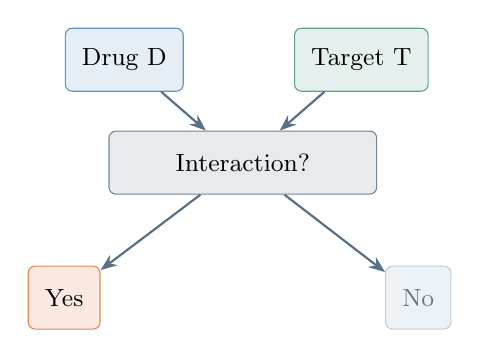
\begin{tikzpicture}[node distance=7mm]
        \node[drug]                       (d) {\e{Drug D}};
        \node[targ, right=14mm of d]      (t) {\e{Target T}};
        \node[model, below=9mm of $(d)!0.5!(t)$, minimum width=34mm] (i) {\e{Interaction?}};
        \node[res,  below left=9mm and 1mm of i]  (y) {\e{Yes}};
        \node[ghost,below right=9mm and 1mm of i] (n) {\e{No}};
        \draw[arr] (d) -- (i);
        \draw[arr] (t) -- (i);
        \draw[arr] (i) -- (y);
        \draw[arr] (i) -- (n);
      \end{tikzpicture}
    \end{column}
  \end{columns}
  \note{\e{DTI} را به عنوان مسئله‌ی پایه معرفی کن: «اگر بخواهیم فضای جستجوی \e{drug discovery} را کوچک کنیم، اولین سؤال این است که از میان تعداد زیادی دارو و پروتئین، کدام جفت‌ها احتمالاً با هم برهم‌کنش دارند.» مقاله‌ی \e{Co-VAE} هم مقدمه‌اش را از همین نقطه شروع می‌کند.}
\end{frame}

%---------------------------------------------------------------- 2 --
\begin{frame}{از تشخیص برهم‌کنش به اندازه‌گیری قدرت آن}
  \framesubtitle{چرا پاسخ بله/خیر کافی نیست؟}
  \vspace{1mm}
  \centering
  \begin{tikzpicture}[x=1mm,y=1mm,font=\footnotesize]
    % --- inputs ---
    \node[drug] (d1) at (0,7)   {\e{Drug A}};
    \node[drug] (d2) at (0,-7)  {\e{Drug B}};
    \node[targ] (tx) at (28,0)  {\e{Target X}};
    \draw[arr] (d1) -- (tx);
    \draw[arr] (d2) -- (tx);

    % --- DTI column ---
    \node[lbl,text=nxdark,font=\scriptsize\bfseries] at (60,17) {\fa{دیدِ \e{DTI}}};
    \node[res,minimum width=26mm]   (y1) at (60,7)  {\e{Yes}};
    \node[res,minimum width=26mm]   (y2) at (60,-7) {\e{Yes}};
    \draw[arr] (tx) -- (y1);
    \draw[arr] (tx) -- (y2);
    \node[lbl,text width=32mm,align=center] at (60,-17) {\fa{هر دو یکسان دیده می‌شوند}};

    % --- divider ---
    \draw[nxdark!20,thick] (80,20) -- (80,-20);

    % --- DTA column ---
    \node[lbl,text=nxdark,font=\scriptsize\bfseries] at (104,17) {\fa{دیدِ \e{DTA}}};
    \node[nxn,minimum width=28mm,fill=nxred!18,draw=nxred!80] (s1) at (104,7)  {\e{Strong binding}};
    \node[ghost,minimum width=28mm]                           (s2) at (104,-7) {\e{Weak binding}};
    \draw[arr,draw=nxdark!35] (y1) -- (s1);
    \draw[arr,draw=nxdark!35] (y2) -- (s2);
    \node[lbl,text width=34mm,align=center] at (104,-17) {\fa{دو دارو از هم تفکیک می‌شوند}};
  \end{tikzpicture}

  \vspace{2mm}
  \begin{alertblock}{پرسش دقیق‌تر}
    \centering قدرت اتصال دارو به هدف \key{چقدر} است؟ \quad$\Rightarrow$\quad مسئله‌ی \E{Drug--Target Binding Affinity (DTA)}
  \end{alertblock}
  \note{نکته‌ی کلیدی: دو دارو می‌توانند هر دو با یک \e{target} برهم‌کنش داشته باشند، ولی یکی اتصال بسیار قوی و دیگری اتصال ضعیف. \e{DTI} این تفاوت را نمی‌بیند. اینجا گذار از مسئله‌ی دسته‌بندی به مسئله‌ی رگرسیون اتفاق می‌افتد.}
\end{frame}

%---------------------------------------------------------------- 3 --
\begin{frame}{چرا \e{DTA}؟}
  \framesubtitle{اطلاعات کمی در برابر اطلاعات دودویی}
  \vspace{2mm}
  \centering
  {\small
  \rowcolors{2}{nxlight}{white}
  \begin{tabular}{p{0.34\textwidth} p{0.34\textwidth}}
    \rowcolor{nxdark}
    \thd{\e{DTI}} & \thd{\e{DTA}} \\
    آیا برهم‌کنش وجود دارد؟ & برهم‌کنش چقدر قوی است؟ \\
    خروجی دودویی (\e{binary})   & خروجی پیوسته (\e{continuous}) \\
    بله / خیر                & مقدار عددی \e{affinity} \\
    مناسب غربالگری اولیه     & مناسب رتبه‌بندی و اولویت‌دهی \\
  \end{tabular}}

  \vspace{4mm}
  \begin{columns}[c]
    \begin{column}{0.55\textwidth}
      \begin{exampleblock}{جمله‌ی کلیدی}
        \e{DTA} علاوه بر \key{وجود} برهم‌کنش، \key{شدت} آن را نیز مشخص می‌کند و
        بنابراین اطلاعات غنی‌تری در اختیار می‌گذارد.
      \end{exampleblock}
    \end{column}
    \begin{column}{0.42\textwidth}
      {\footnotesize\color{nxgray}
       \textbf{دقت در بیان:} نگوییم «\e{DTA} همیشه بهتر از \e{DTI} است»؛
       این‌ها دو صورت‌بندی متفاوت از مسئله‌اند. بگوییم برای \emph{هدف این پژوهش}،
       اطلاعات کمی \e{affinity} ارزشمندتر است.}
    \end{column}
  \end{columns}
  \note{حتماً تأکید کن که \e{DTA} و \e{DTI} دو \e{formulation} متفاوت‌اند، نه اینکه یکی مطلقاً بهتر از دیگری باشد. این جمله از نظر علمی قابل دفاع‌تر است و معمولاً همین‌جا سؤال پرسیده می‌شود. \e{Co-VAE} هم پیش‌بینی \e{affinity} را چالش‌برانگیزتر از تشخیص \e{interaction} می‌داند.}
\end{frame}

%---------------------------------------------------------------- 4 --
\begin{frame}{قدرت اتصال چگونه اندازه‌گیری می‌شود؟}
  \framesubtitle{نقشه‌ی معیارهای متداول}
  \vspace{4mm}
  \centering
  \begin{tikzpicture}[node distance=5mm]
    \node[model,minimum width=30mm] (root) {\fa{اندازه‌گیری \e{Affinity}}};

    \node[targ,minimum width=44mm,below right=12mm and 2mm of root] (ba) {\e{Binding affinity}\\[-1mm] \fa{{\scriptsize قدرت اتصال ترمودینامیکی}}};
    \node[res, minimum width=40mm,below left=12mm and 2mm of root]  (po) {\e{Potency / inhibition}\\[-1mm] \fa{{\scriptsize اثر عملکردی در آزمایش}}};

    \node[nxn,below left=10mm and -2mm of ba]  (kd) {\e{Kd} \ / \ \e{pKd}};
    \node[nxn,below right=10mm and -2mm of ba] (ki) {\e{Ki} \ / \ \e{pKi}};
    \node[nxn,below=10mm of po]                (ic) {\e{IC50}};

    \draw[arr] (root) -- (ba);
    \draw[arr] (root) -- (po);
    \draw[arr] (ba) -- (kd);
    \draw[arr] (ba) -- (ki);
    \draw[arr] (po) -- (ic);
  \end{tikzpicture}

  \vspace{3mm}
  {\footnotesize\color{nxgray}
   در اسلایدهای بعد هر معیار جداگانه تعریف می‌شود؛ تمایز ستون راست و چپ نکته‌ی اصلی این بخش است.}
  \note{این اسلاید «نقشه» است. فقط بگو چهار پنج اصطلاح داریم و مهم‌ترین نکته این است که \e{Kd} و \e{Ki} معیار \e{binding affinity} هستند ولی \e{IC50} معیار \e{potency} عملکردی است. جزئیات را در اسلایدهای بعد باز می‌کنی.}
\end{frame}

%---------------------------------------------------------------- 5 --
\begin{frame}{\e{Kd} و \e{pKd}}
  \framesubtitle{\e{Equilibrium Dissociation Constant}}
  \vspace{1mm}
  \begin{columns}[T]
    \begin{column}{0.50\textwidth}
      \small
      \begin{block}{تعریف مفهومی}
        \e{Kd} غلظتی از \e{ligand} است که در شرایط تعادل، تقریباً \key{نیمی} از
        \e{target}ها را در حالت \e{bound} قرار می‌دهد.
      \end{block}

      \vspace{-1mm}
      \disp{K_d \;=\; \frac{[D]\,[T]}{[DT]}}

      \vspace{-3mm}
      {\footnotesize
      \e{D}: داروی آزاد \quad $\cdot$ \quad \e{T}: هدف آزاد \quad $\cdot$ \quad \e{DT}: کمپلکس دارو--هدف}

      \vspace{2mm}
      \begin{alertblock}{مقیاس لگاریتمی}
        \vspace{-3mm}
        \disp{pK_d \;=\; -\log_{10}\!\big(K_d\,[M]\big)}
        \vspace{-3mm}
        \centering اگر \lr{$K_d = 10^{-9}\,M$} آنگاه \lr{$pK_d = 9$}
      \end{alertblock}
    \end{column}

    \begin{column}{0.46\textwidth}
      \centering
      \vspace{3mm}
      % مقیاس به‌صورت راست‌به‌چپ خوانده می‌شود: سمت راست = اتصال قوی
      \begin{tikzpicture}
        \shade[left color=nxlight,right color=nxred!55] (0,0) rectangle (6.4,0.55);
        \draw[nxdark!35] (0,0) rectangle (6.4,0.55);
        \node[lbl,below] at (5.8,0) {\fa{\e{Kd} کوچک}};
        \node[lbl,below] at (0.6,0) {\fa{\e{Kd} بزرگ}};
        \node[lbl,above,text=nxdark,font=\scriptsize\bfseries] at (5.4,0.55) {\fa{اتصال قوی}};
        \node[lbl,above,text=nxdark,font=\scriptsize\bfseries] at (1.0,0.55) {\fa{اتصال ضعیف}};

        \node[drug,minimum width=24mm,below=11mm of {(5.4,0)},font=\scriptsize] (a)
          {\e{Drug A}\\[-1mm]{\scriptsize\e{Kd = 1 nM}}};
        \node[ghost,minimum width=24mm,below=11mm of {(1.0,0)},font=\scriptsize] (b)
          {\e{Drug B}\\[-1mm]{\scriptsize\e{Kd = 100 nM}}};
      \end{tikzpicture}

      \vspace{6mm}
      {\small\color{nxdark}
       \lr{$K_d \downarrow$} \quad$\Longrightarrow$\quad \e{affinity} \lr{$\uparrow$} \quad$\Longrightarrow$\quad \lr{$pK_d \uparrow$}}
    \end{column}
  \end{columns}
  \note{نکته‌ای که معمولاً پرسیده می‌شود: چرا لگاریتم می‌گیریم؟ چون مقادیر \e{Kd} در بازه‌ای بسیار وسیع و بسیار کوچک (نانومولار تا میکرومولار) پخش‌اند و مقیاس لگاریتمی هم عددها را قابل‌مدیریت می‌کند و هم برای رگرسیون مناسب‌تر است. جهت را اشتباه نگو: \e{Kd} کمتر یعنی \e{affinity} بیشتر.}
\end{frame}

%---------------------------------------------------------------- 6 --
\begin{frame}{\e{Ki} و \e{pKi}}
  \framesubtitle{\e{Inhibition Constant}}
  \vspace{2mm}
  \begin{columns}[T]
    \begin{column}{0.50\textwidth}
      \small
      \begin{block}{تعریف}
        \e{Ki} معیاری برای بیان \e{affinity} یک \key{مهارکننده} (\e{inhibitor})
        نسبت به \e{target} یا آنزیم است.
      \end{block}

      \vspace{1mm}
      هرچه \e{Ki} کوچک‌تر باشد، \e{inhibitor} تمایل بیشتری به اتصال مؤثر
      به \e{target} دارد.

      \vspace{-1mm}
      \disp{pK_i \;=\; -\log_{10}\!\big(K_i\,[M]\big)}

      \vspace{-2mm}
      \centering
      {\small \lr{$K_i \downarrow$} \quad$\Longrightarrow$\quad \lr{$pK_i \uparrow$} \quad$\Longrightarrow$\quad \e{affinity} \lr{$\uparrow$}}
    \end{column}

    \begin{column}{0.46\textwidth}
      \vspace{2mm}
      \begin{alertblock}{\e{Ki} و \e{Kd} یکی نیستند}
        \small
        \begin{itemize}
          \item \E{Kd}: مستقیماً \e{equilibrium dissociation} را در یک سامانه‌ی اتصال بیان می‌کند.
          \item \E{Ki}: در زمینه‌ی \e{inhibition} و برای بیان \e{potency/affinity} مهارکننده به کار می‌رود.
        \end{itemize}
      \end{alertblock}

      \vspace{1mm}
      {\footnotesize\color{nxgray}
       هر دو در ادبیات \e{DTA} به عنوان برچسب \e{affinity} استفاده می‌شوند؛
       مجموعه‌داده‌های مختلف برچسب‌های متفاوتی دارند.}
    \end{column}
  \end{columns}
  \note{اگر استاد پرسید تفاوت \e{Ki} و \e{Kd} چیست، همین اسلاید جواب است. اضافه کن که در عمل، مجموعه‌داده‌ها فرق دارند: \e{Davis} بر پایه‌ی \e{Kd} است و \e{KIBA} یک امتیاز ترکیبی است؛ بنابراین مقایسه‌ی اعداد بین مجموعه‌داده‌ها مستقیماً معنادار نیست.}
\end{frame}

%---------------------------------------------------------------- 7 --
\begin{frame}{\e{IC50}}
  \framesubtitle{\e{Half Maximal Inhibitory Concentration}}
  \vspace{1mm}
  \begin{columns}[T]
    \begin{column}{0.44\textwidth}
      \small
      \vspace{2mm}
      \begin{block}{تعریف}
        غلظتی از \e{inhibitor} که باعث \key{۵۰٪ کاهش} فعالیت یک سامانه یا
        آنزیم می‌شود.
      \end{block}

      \vspace{2mm}
      \begin{alertblock}{نکته‌ی مهم علمی}
        \e{IC50} مستقیماً \key{معیار \e{binding affinity} نیست}؛
        یک معیار \e{functional inhibition / potency} است و به شرایط
        آزمایش (مثلاً غلظت \e{substrate}) وابسته است.
      \end{alertblock}
    \end{column}

    \begin{column}{0.52\textwidth}
      \centering
      \vspace{4mm}
      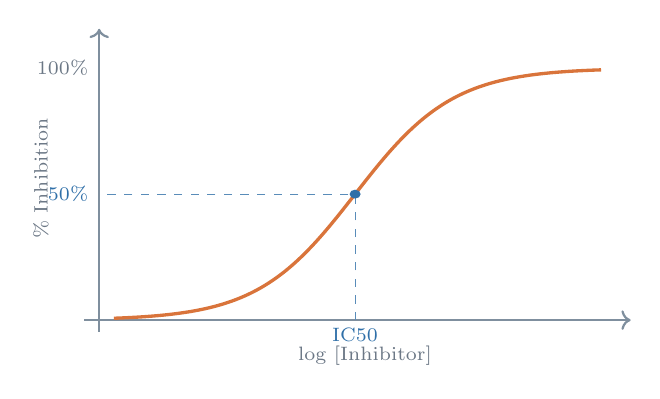
\begin{tikzpicture}[xscale=1.25,yscale=1.0]
        \draw[->,nxdark!55,thick] (-0.15,0) -- (5.4,0);
        \draw[->,nxdark!55,thick] (0,-0.15) -- (0,3.7);
        \node[lbl,below] at (2.7,-0.25) {\e{log [Inhibitor]}};
        \node[lbl,rotate=90,above] at (-0.45,1.8) {\e{\% Inhibition}};

        \draw[nxaccent,very thick] plot[domain=0.15:5.1,samples=90,smooth]
             (\x,{3.2/(1+exp(-2.0*(\x-2.6)))});

        \draw[dashed,nxblue!80] (2.6,0) -- (2.6,1.6) -- (0,1.6);
        \fill[nxblue] (2.6,1.6) circle (1.6pt);
        \node[lbl,text=nxblue,below] at (2.6,-0.02) {\e{IC50}};
        \node[lbl,text=nxblue,left]  at (-0.05,1.6) {\e{50\%}};
        \node[lbl,left] at (-0.05,3.2) {\e{100\%}};
      \end{tikzpicture}

      \vspace{2mm}
      {\footnotesize\color{nxgray}
       منحنی پاسخ به غلظت؛ \e{IC50} نقطه‌ی رسیدن به نیمه‌ی حداکثر مهار است.}
    \end{column}
  \end{columns}
  \note{این تمایز را حتماً بگو، چون از نظر علمی مهم است و نشان می‌دهد ادبیات را دقیق خوانده‌ای: \e{Kd} و \e{Ki} معیار اتصال‌اند، \e{IC50} معیار اثر عملکردی. ادبیات مقایسه‌ی ابزارهای \e{DTA} هم صراحتاً روی همین تأکید می‌کند.}
\end{frame}

%---------------------------------------------------------------- 8 --
\begin{frame}{جمع‌بندی معیارهای اتصال و مهار}
  \framesubtitle{کدام معیار چه چیزی را می‌سنجد؟}
  \vspace{3mm}
  \centering
  {\small
  \rowcolors{2}{nxlight}{white}
  \begin{tabular}{p{0.16\textwidth} p{0.34\textwidth} p{0.28\textwidth}}
    \rowcolor{nxdark}
    \thd{معیار} & \thd{مفهوم} & \thd{مقدار کمتر یعنی} \\
    \E{Kd}   & \e{Dissociation constant}        & \e{affinity} بیشتر \\
    \E{pKd}  & \e{−log\textsubscript{10}(K\textsubscript{d})} & \e{affinity} بیشتر \\
    \E{Ki}   & \e{Inhibition constant}          & \e{affinity} بیشتر \\
    \E{pKi}  & \e{−log\textsubscript{10}(K\textsubscript{i})} & \e{affinity} بیشتر \\
    \E{IC50} & غلظت لازم برای ۵۰٪ مهار          & \e{potency} بیشتر \\
  \end{tabular}}

  \vspace{5mm}
  \begin{exampleblock}{کاربرد در عمل}
    در بسیاری از \e{benchmark}های \e{DTA}، مقادیر \e{affinity} به شکل
    \key{لگاریتمی} مانند \e{pKd} یا \e{pKi} استفاده می‌شوند.
    برای نمونه \e{DCGAN-DTA} روی \e{BindingDB} مقادیر را به \e{pKd} تبدیل کرده
    و \e{PDBBind} نیز شامل مقادیر \e{log-transformed} از \e{Ki} و \e{Kd} است.
  \end{exampleblock}
  \note{این اسلاید پل به بخش بعد است. بگو: «پس برچسبی که مدل‌ها پیش‌بینی می‌کنند معمولاً یک عدد پیوسته در مقیاس لگاریتمی است؛ حالا ببینیم پژوهشگران برای پیش‌بینی این عدد چه مسیری را طی کرده‌اند.»}
\end{frame}

%======================================================================
\section{مسیر پژوهشی}
%======================================================================

%---------------------------------------------------------------- 9 --
\begin{frame}{درخت تکاملی روش‌های پیش‌بینی \e{DTA}}
  \framesubtitle{از ۲۰۱۵ تا ۲۰۲۶ --- بر پایه‌ی مرور \e{Wang et al.}, \e{Biotechnology Advances}, ۲۰۲۶}
  \vspace{1mm}
  \centering
  \begin{tikzpicture}[x=1mm,y=1mm,
      tn/.style={nxn,minimum height=6.6mm,inner xsep=3pt,inner ysep=1.5pt,
                 font=\tiny,align=center},
      bus/.style={draw=nxdark!65,thick},
      dn/.style={-{Stealth[length=1.8mm,width=1.4mm]},draw=nxdark!65,thick}]

    % ---- tier A: the historical spine --------------------------------
    \node[tn,ghost,minimum width=34mm] (a1) at (22,27)  {\fa{شباهت و \e{Kernel}}\\\e{KronRLS} --- ۲۰۱۵};
    \node[tn,ghost,minimum width=34mm] (a2) at (64,27)  {\fa{یادگیری ماشین ویژگی‌محور}\\\e{SimBoost} --- ۲۰۱۷};
    \node[tn,model,minimum width=34mm] (a3) at (106,27) {\fa{یادگیری عمیق}\\\e{DeepDTA} --- ۲۰۱۸};
    \draw[dn] (a1)--(a2); \draw[dn] (a2)--(a3);

    % ---- tier B: three representation families -----------------------
    \node[tn,minimum width=34mm] (b1) at (22,12)  {\fa{توالی و} \e{CNN}\\\e{DeepDTA} $\cdot$ \e{WideDTA}};
    \node[tn,minimum width=34mm] (b2) at (64,12)  {\fa{گراف و} \e{GNN}\\\e{GraphDTA} $\cdot$ \e{MGraphDTA}};
    \node[tn,minimum width=34mm] (b3) at (106,12) {\fa{توجه و} \e{Transformer}\\\e{AttentionDTA} $\cdot$ \e{ELECTRA-DTA}};
    \draw[bus] (a3.south) -- (106,20);
    \draw[bus] (22,20) -- (106,20);
    \draw[dn] (22,20) -- (b1.north);
    \draw[dn] (64,20) -- (b2.north);
    \draw[dn] (106,20) -- (b3.north);

    % ---- tier C: representation learning -----------------------------
    \node[tn,model,minimum width=66mm] (rep) at (64,0)
      {\fa{یادگیری نمایش} --- \e{Representation Learning}};
    \draw[bus] (b1.south) -- (22,5.5);
    \draw[bus] (b2.south) -- (64,5.5);
    \draw[bus] (b3.south) -- (106,5.5);
    \draw[bus] (22,5.5) -- (106,5.5);
    \draw[dn] (64,5.5) -- (rep.north);

    % ---- tier D: three sibling branches of representation learning ---
    \node[tn,minimum width=34mm] (d1) at (22,-13)  {\fa{ترکیب چندوجهی}\\\e{Fusion} $\cdot$ \e{Multimodal}};
    \node[tn,res,minimum width=34mm,draw=nxaccent,line width=0.7pt] (d2) at (64,-13)
      {\fa{یادگیری نمایش مولد}\\\e{Generative}};
    \node[tn,minimum width=34mm] (d3) at (106,-13) {\fa{پیش‌آموزش‌دیده}\\\e{Protein} \& \e{Chemical LM}};
    \draw[bus] (rep.south) -- (64,-7);
    \draw[bus] (22,-7) -- (106,-7);
    \draw[dn] (22,-7) -- (d1.north);
    \draw[dn] (64,-7) -- (d2.north);
    \draw[dn] (106,-7) -- (d3.north);

    % ---- tier E: the two papers this thesis studies -------------------
    \node[tn,minimum width=32mm,fill=nxblue!25,draw=nxblue,line width=0.7pt,
          font=\tiny\bfseries] (e1) at (44,-27) {\e{GAN} $\rightarrow$ \e{DCGAN-DTA} --- ۲۰۲۴};
    \node[tn,minimum width=32mm,fill=nxteal!25,draw=nxteal,line width=0.7pt,
          font=\tiny\bfseries] (e2) at (84,-27) {\e{VAE} $\rightarrow$ \e{Co-VAE} --- ۲۰۲۲};
    \draw[bus] (d2.south) -- (64,-20);
    \draw[bus] (44,-20) -- (84,-20);
    \draw[dn] (44,-20) -- (e1.north);
    \draw[dn] (84,-20) -- (e2.north);
  \end{tikzpicture}

  \vspace{1mm}
  {\scriptsize\color{nxgray}
   هر شاخه پاسخی به یک محدودیت متفاوت است --- \key{نه جانشین کامل نسل قبلی}.
   دو برگ پررنگ، نقطه‌ی ورود این پایان‌نامه‌اند.}
  \note{مهم‌ترین اسلاید بخش دوم؛ حدود دو تا سه دقیقه رویش وقت بگذار. دو پیام اصلی: (۱) این یک زنجیره‌ی خطی نیست، یک درخت است و شاخه‌های پایینی هم‌زمان‌اند نه پشت سر هم؛ (۲) \e{Generative} یک شاخه‌ی هم‌رده‌ی \e{Fusion} و \e{Pre-trained} است، نه مرحله‌ی بعد از \e{GNN}. در پایان انگشت بگذار روی دو برگ پررنگ و بگو «پایان‌نامه دقیقاً اینجاست».}
\end{frame}

%--------------------------------------------------------------- 10 --
\begin{frame}{مرحله‌ی اول: شباهت و \e{Kernel}}
  \framesubtitle{\e{KronRLS} --- \e{Pahikkala et al.}, ۲۰۱۵}
  \vspace{2mm}
  \begin{columns}[T]
    \begin{column}{0.50\textwidth}
      \small
      \begin{block}{فرض اصلی این نسل}
        اگر دو دارو از نظر شیمیایی شبیه باشند، احتمالاً \e{affinity} مشابهی
        دارند؛ پروتئین‌های مشابه نیز الگوی \e{binding} مشابهی دارند.
      \end{block}

      \vspace{1mm}
      \begin{exampleblock}{\e{KronRLS}}
        \small
        \e{Kronecker Regularized Least Squares} --- شباهت دارو--دارو و
        هدف--هدف را ترکیب می‌کند و مسئله را در قالب
        \e{regularized least squares} حل می‌کند.
      \end{exampleblock}
    \end{column}

    \begin{column}{0.46\textwidth}
      \centering
      \begin{tikzpicture}[x=1mm,y=1mm,font=\scriptsize]
        \node[drug,minimum width=25mm]  (s1) at (0,14)   {\fa{شباهت دارو}};
        \node[targ,minimum width=25mm]  (s2) at (30,14)  {\fa{شباهت پروتئین}};
        \node[model,minimum width=36mm] (k)  at (15,2)   {\e{Kernel} / \e{KronRLS}};
        \node[res,minimum width=25mm]   (a)  at (15,-11) {\e{Affinity}};
        \draw[arr] (s1)--(k); \draw[arr] (s2)--(k); \draw[arr] (k)--(a);
      \end{tikzpicture}

      \vspace{2mm}
      \begin{alertblock}{محدودیت}
        \small مدل فقط به اندازه‌ی کیفیت \e{similarity}ای که \key{انسان}
        تعریف کرده خوب بود؛ نمایش هنوز دستی و از پیش تعریف‌شده است.
      \end{alertblock}
    \end{column}
  \end{columns}
  \note{کوتاه رد شو. پیام: کیفیت مدل عملاً برابر بود با کیفیت تابع شباهتی که انسان تعریف می‌کرد. \e{KronRLS} هنوز هم یکی از \e{baseline}های استاندارد است و \e{DeepDTA} مستقیماً با آن مقایسه می‌شود.}
\end{frame}

%--------------------------------------------------------------- 11 --
\begin{frame}{مرحله‌ی دوم: یادگیری ماشین ویژگی‌محور}
  \framesubtitle{\e{SimBoost} --- \e{He et al.}, ۲۰۱۷}
  \vspace{2mm}
  \begin{columns}[T]
    \begin{column}{0.48\textwidth}
      \small
      \begin{block}{ویژگی‌های صریح به جای شباهت صرف}
        \begin{itemize}\itemsep0.2ex
          \item دارو: \e{fingerprints}، \e{descriptors}، ویژگی‌های ساختاری دوبعدی
          \item پروتئین: شباهت توالی، ویژگی‌های فیزیکوشیمیایی، اطلاعات تکاملی
          \item جفت دارو--هدف: ویژگی‌های شبکه‌ای
        \end{itemize}
      \end{block}

      \vspace{1mm}
      {\footnotesize
       \e{SimBoost} به جای \e{kernel} ساده از \E{Gradient Boosting Machines}
       استفاده کرد و توانست روابط \key{غیرخطی‌تر} را مدل کند.}
    \end{column}

    \begin{column}{0.48\textwidth}
      \centering
      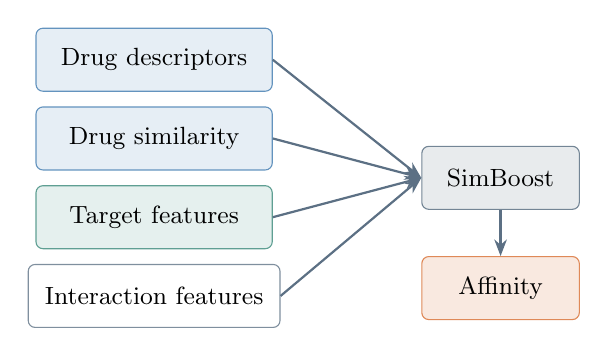
\begin{tikzpicture}[x=1mm,y=1mm,font=\scriptsize]
        \node[drug,minimum width=30mm]  (f1) at (0,16)  {\e{Drug descriptors}};
        \node[drug,minimum width=30mm]  (f2) at (0,6)   {\e{Drug similarity}};
        \node[targ,minimum width=30mm]  (f3) at (0,-4)  {\e{Target features}};
        \node[nxn,minimum width=30mm]   (f4) at (0,-14) {\e{Interaction features}};
        \node[model,minimum width=20mm] (sb) at (44,1)  {\e{SimBoost}};
        \node[res,minimum width=20mm]   (af) at (44,-13) {\e{Affinity}};
        \draw[arr] (f1.east) -- (sb.west);
        \draw[arr] (f2.east) -- (sb.west);
        \draw[arr] (f3.east) -- (sb.west);
        \draw[arr] (f4.east) -- (sb.west);
        \draw[arr] (sb) -- (af);
      \end{tikzpicture}

      \vspace{2mm}
      \begin{alertblock}{گلوگاه جابه‌جا شد}
        \small از \e{Similarity Engineering} به \key{\e{Feature Engineering}} ---
        ولی هنوز انسان در حلقه است.
      \end{alertblock}
    \end{column}
  \end{columns}
  \note{پیام کوتاه: پیشرفت واقعی بود (مدل‌سازی غیرخطی)، ولی گلوگاه فقط یک قدم عقب‌تر رفت. این همان چیزی است که یادگیری عمیق در مرحله‌ی بعد حذفش می‌کند.}
\end{frame}

%--------------------------------------------------------------- 12 --
\begin{frame}{مرحله‌ی سوم: ورود یادگیری عمیق}
  \framesubtitle{\e{DeepDTA} --- \e{Öztürk et al.}, ۲۰۱۸ \quad$\cdot$\quad \e{WideDTA}, ۲۰۱۹}
  \vspace{2mm}
  \centering
  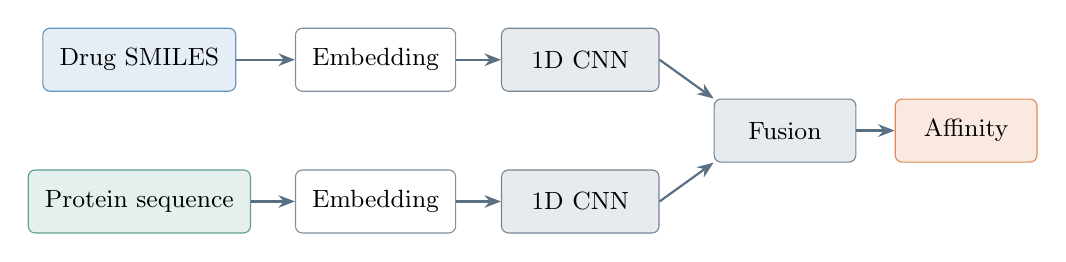
\begin{tikzpicture}[x=1mm,y=1mm,font=\scriptsize]
    \node[drug,minimum width=24mm]  (sm) at (12,10)  {\e{Drug SMILES}};
    \node[targ,minimum width=24mm]  (pr) at (12,-8)  {\e{Protein sequence}};
    \node[nxn,minimum width=20mm]   (e1) at (42,10)  {\e{Embedding}};
    \node[nxn,minimum width=20mm]   (e2) at (42,-8)  {\e{Embedding}};
    \node[model,minimum width=20mm] (c1) at (68,10)  {\e{1D CNN}};
    \node[model,minimum width=20mm] (c2) at (68,-8)  {\e{1D CNN}};
    \node[model,minimum width=18mm] (fu) at (94,1)   {\e{Fusion}};
    \node[res,minimum width=18mm]   (af) at (117,1)  {\e{Affinity}};
    \draw[arr] (sm)--(e1); \draw[arr] (e1)--(c1);
    \draw[arr] (pr)--(e2); \draw[arr] (e2)--(c2);
    \draw[arr] (c1.east) -- (fu.north west);
    \draw[arr] (c2.east) -- (fu.south west);
    \draw[arr] (fu)--(af);
  \end{tikzpicture}

  \vspace{3mm}
  \begin{columns}[T]
    \begin{column}{0.48\textwidth}
      \begin{alertblock}{تغییر بنیادی}
        \small
        نمایش دیگر به‌طور کامل توسط انسان تعریف نمی‌شود؛
        \key{شبکه آن را از داده‌ی خام یاد می‌گیرد}.
      \end{alertblock}
    \end{column}
    \begin{column}{0.48\textwidth}
      \begin{exampleblock}{\e{WideDTA} --- گام بعدی}
        \small
        افزودن \e{protein domains/motifs} و
        \e{maximum common substructure} برای نمایشی غنی‌تر.
      \end{exampleblock}
    \end{column}
  \end{columns}
  \note{\e{DeepDTA} نقطه‌ی عطف این حوزه است و تقریباً همه‌ی مقالات بعدی با آن مقایسه می‌شوند. اگر وقت کم بود، فقط همین اسلاید را از کل بخش بگو.}
\end{frame}

%--------------------------------------------------------------- 13 --
\begin{frame}{مرحله‌ی چهارم: گراف و نمایش ساختارآگاه}
  \framesubtitle{\e{GraphDTA} --- \e{Nguyen et al.}, ۲۰۲۱}
  \vspace{2mm}
  \begin{columns}[T]
    \begin{column}{0.50\textwidth}
      \centering
      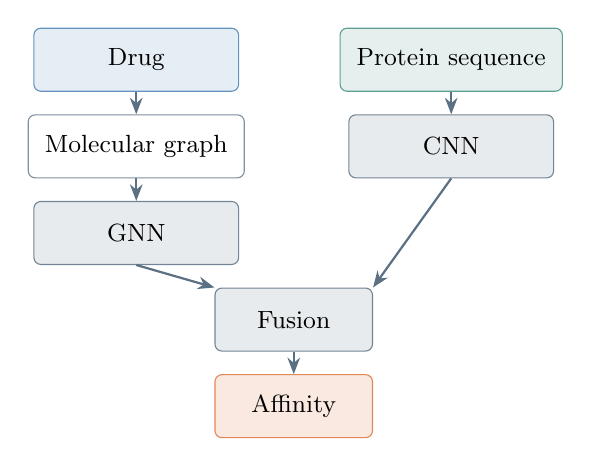
\begin{tikzpicture}[x=1mm,y=1mm,font=\scriptsize]
        \node[drug,minimum width=26mm]  (d)  at (0,18)  {\e{Drug}};
        \node[nxn,minimum width=26mm]   (g)  at (0,7)   {\e{Molecular graph}};
        \node[model,minimum width=26mm] (gn) at (0,-4)  {\e{GNN}};
        \node[targ,minimum width=26mm]  (p)  at (40,18) {\e{Protein sequence}};
        \node[model,minimum width=26mm] (cn) at (40,7)  {\e{CNN}};
        \node[model,minimum width=20mm] (fu) at (20,-15) {\e{Fusion}};
        \node[res,minimum width=20mm]   (af) at (20,-26) {\e{Affinity}};
        \draw[arr] (d)--(g); \draw[arr] (g)--(gn);
        \draw[arr] (p)--(cn);
        \draw[arr] (gn.south) -- (fu.north west);
        \draw[arr] (cn.south) -- (fu.north east);
        \draw[arr] (fu)--(af);
      \end{tikzpicture}
    \end{column}

    \begin{column}{0.46\textwidth}
      \small
      \begin{block}{چرا گراف؟}
        \e{SMILES} فقط یک \key{سریال‌سازی} از مولکول است، در حالی که مولکول
        ذاتاً یک گراف است: اتم $\rightarrow$ \e{Node}، پیوند $\rightarrow$ \e{Edge}.
      \end{block}

      \vspace{1mm}
      {\footnotesize
       \e{GraphDTA} چند معماری را بررسی کرد:
       \e{GCN} $\cdot$ \e{GAT} $\cdot$ \e{GAT-GCN} $\cdot$ \e{GIN}.}

      \vspace{2mm}
      \begin{exampleblock}{نتیجه}
        \small مسئله فقط عمیق‌تر کردن شبکه نبود؛ \key{نوع نمایش} هم تغییر کرد:
        از \e{sequence representation} به \e{structure-aware representation}.
      \end{exampleblock}
    \end{column}
  \end{columns}
  \note{اگر پرسیده شد چرا گراف بهتر است: چون اطلاعات ساختاری (حلقه‌ها، شاخه‌ها، همسایگی اتم‌ها) در \e{SMILES} به‌صورت ضمنی و در گراف به‌صورت صریح کد می‌شود. وارد جزئیات \e{GNN} نشو، موضوع پایان‌نامه نیست.}
\end{frame}

%--------------------------------------------------------------- 14 --
\begin{frame}{مرحله‌ی پنجم: توجه و \e{Transformer}}
  \framesubtitle{\e{AttentionDTA} $\cdot$ \e{ELECTRA-DTA} $\cdot$ \e{FusionDTA}, ۲۰۲۲}
  \vspace{2mm}
  \begin{columns}[T]
    \begin{column}{0.48\textwidth}
      \small
      \begin{block}{پرسش تازه}
        حتی با نمایش خوب، هنوز باید مشخص شود \key{کدام بخش} از دارو و
        کدام بخش از پروتئین برای \e{binding} مهم‌تر است.
      \end{block}

      \vspace{1mm}
      \begin{exampleblock}{\e{FusionDTA}}
        \small
        تمرکز بر \e{feature aggregation} با
        \e{attention-based feature polymerization} و
        \e{knowledge distillation}.
      \end{exampleblock}
    \end{column}

    \begin{column}{0.48\textwidth}
      \centering
      \vspace{1mm}
      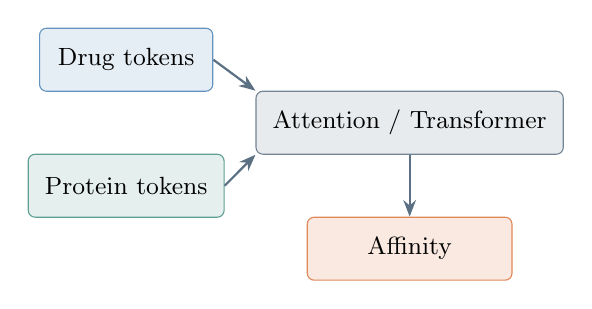
\begin{tikzpicture}[x=1mm,y=1mm,font=\scriptsize]
        \node[drug,minimum width=22mm]  (d) at (0,12)  {\e{Drug tokens}};
        \node[targ,minimum width=22mm]  (p) at (0,-4)  {\e{Protein tokens}};
        \node[model,minimum width=30mm] (at) at (36,4) {\e{Attention} / \e{Transformer}};
        \node[res,minimum width=26mm]   (af) at (36,-12) {\e{Affinity}};
        \draw[arr] (d.east) -- (at.north west);
        \draw[arr] (p.east) -- (at.south west);
        \draw[arr] (at)--(af);
      \end{tikzpicture}

      \vspace{2mm}
      {\footnotesize\color{nxgray}
       \e{CNN} برای الگوهای \e{local} مناسب است؛ \e{attention} می‌تواند
       وابستگی‌های دوربرد و میان‌وجهی را مدل کند.}
    \end{column}
  \end{columns}

  \vspace{1mm}
  \centering
  {\footnotesize
   تمرکز از «چه ویژگی‌ای استخراج کنیم؟» به
   \key{«چگونه ویژگی‌ها را با هم تعامل دهیم؟»} منتقل شد.}
  \note{این مرحله در نسخه‌ی قبلی ارائه غایب بود. نکته‌ی کلیدی: \e{attention} یک نوع نمایش جدید نمی‌سازد، بلکه نحوه‌ی ترکیب نمایش‌های موجود را یاد می‌گیرد.}
\end{frame}

%--------------------------------------------------------------- 15 --
\begin{frame}{مرحله‌ی ششم: چندوجهی و مدل‌های پیش‌آموزش‌دیده}
  \framesubtitle{\e{Multi-modal fusion} و \e{Protein/Chemical Language Models}}
  \vspace{2mm}
  \begin{columns}[T]
    \begin{column}{0.44\textwidth}
      \small
      \begin{block}{یک نمایش کافی نیست}
        \begin{itemize}\itemsep0.2ex
          \item دارو: \e{SMILES}، گراف مولکولی، \e{descriptors}
          \item پروتئین: توالی، ساختار، \e{binding site}، اطلاعات تکاملی
        \end{itemize}
      \end{block}

      \vspace{1mm}
      {\footnotesize
       نمونه‌ها: \e{DeepFusionDTA} $\cdot$ \e{MDF-DTA} $\cdot$
       \e{PocketDTA} $\cdot$ \e{GraphTransDTA}}
    \end{column}

    \begin{column}{0.52\textwidth}
      \centering
      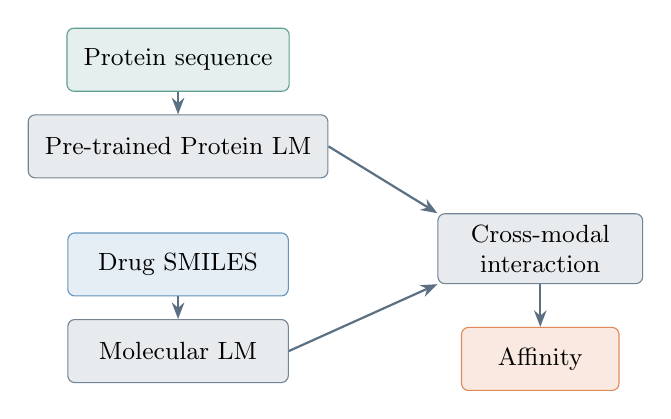
\begin{tikzpicture}[x=1mm,y=1mm,font=\scriptsize]
        \node[targ,minimum width=28mm]  (ps) at (0,14)  {\e{Protein sequence}};
        \node[model,minimum width=28mm] (pl) at (0,3)   {\e{Pre-trained Protein LM}};
        \node[drug,minimum width=28mm]  (ds) at (0,-12) {\e{Drug SMILES}};
        \node[model,minimum width=28mm] (ml) at (0,-23) {\e{Molecular LM}};
        \node[model,minimum width=26mm] (cx) at (46,-10) {\e{Cross-modal}\\\e{interaction}};
        \node[res,minimum width=20mm]   (af) at (46,-24) {\e{Affinity}};
        \draw[arr] (ps)--(pl); \draw[arr] (ds)--(ml);
        \draw[arr] (pl.east) -- (cx.north west);
        \draw[arr] (ml.east) -- (cx.south west);
        \draw[arr] (cx)--(af);
      \end{tikzpicture}

      \vspace{1mm}
      {\footnotesize\color{nxgray}
       \e{ESM} $\cdot$ \e{ProtBERT} $\cdot$ \e{ChemBERT} --- در مرور ۲۰۲۶،
       مدل‌های پیش‌آموزش‌دیده یک \key{پارادایم مستقل} شمرده می‌شوند.}
    \end{column}
  \end{columns}
  \note{این مرحله هم در نسخه‌ی قبلی غایب بود و اضافه‌کردنش نشان می‌دهد ادبیات را تا ۲۰۲۶ دنبال کرده‌ای. اگر استاد پرسید چرا از این مسیر استفاده نکرده‌ای، بگو موضوع پایان‌نامه شاخه‌ی مولد است و این شاخه‌ی موازی می‌تواند کار آینده باشد.}
\end{frame}

%--------------------------------------------------------------- 16 --
\begin{frame}{مرحله‌ی هفتم: یادگیری نمایش مولد}
  \framesubtitle{شاخه‌ای هم‌رده با \e{Fusion} و \e{Pre-trained} --- نه مرحله‌ی بعد از \e{GNN}}
  \vspace{2mm}
  \begin{columns}[T]
    \begin{column}{0.46\textwidth}
      \small
      \begin{block}{پرسش این شاخه}
        تا اینجا مدل‌ها یک نمایش می‌گیرند و \e{affinity} را پیش‌بینی می‌کنند.
        پرسش تازه: آیا می‌توان از \key{مدل‌های مولد} برای یادگیری
        \key{نمایش بهتر} استفاده کرد؟
      \end{block}

      \vspace{1mm}
      \begin{alertblock}{چرا این شاخه مهم است}
        \small
        \begin{itemize}\itemsep0.2ex
          \item بهره‌گیری از داده‌ی \key{بدون برچسب}
          \item فضای نهان ساختارمند و پیوسته
          \item امکان \e{pretraining} پیش از رگرسیون
        \end{itemize}
      \end{alertblock}
    \end{column}

    \begin{column}{0.50\textwidth}
      \centering
      \vspace{1mm}
      \begin{tikzpicture}[x=1mm,y=1mm,font=\scriptsize]
        \node[res,minimum width=40mm,draw=nxaccent,line width=0.7pt] (gm) at (30,16)
          {\fa{یادگیری نمایش مولد}};
        \node[nxn,minimum width=20mm,fill=nxblue!12,draw=nxblue!75] (gan) at (8,2)  {\E{GAN}};
        \node[nxn,minimum width=20mm,fill=nxteal!12,draw=nxteal!75] (vae) at (52,2) {\E{VAE}};
        \node[nxn,minimum width=26mm,fill=nxblue!25,draw=nxblue,font=\scriptsize\bfseries]
          (dc) at (8,-13) {\e{DCGAN-DTA}};
        \node[nxn,minimum width=26mm,fill=nxteal!25,draw=nxteal,font=\scriptsize\bfseries]
          (cv) at (52,-13) {\e{Co-VAE}};
        \draw[arr] (gm)--(gan); \draw[arr] (gm)--(vae);
        \draw[arr] (gan)--(dc); \draw[arr] (vae)--(cv);
        \node[lbl,text width=26mm,align=center] at (8,-23)  {\fa{یادگیری تخاصمی}};
        \node[lbl,text width=26mm,align=center] at (52,-23) {\fa{یادگیری وردشی}};
      \end{tikzpicture}
    \end{column}
  \end{columns}
  \note{اینجا پل اصلی ارائه است. جمله‌ی گذار: «این دو مقاله دو پاسخ متفاوت به یک پرسش واحدند؛ حالا هر کدام را جداگانه می‌بینیم.» حتماً تأکید کن که \e{Generative} از نظر تاریخی بعد از \e{GNN} نیامده، بلکه یک شاخه‌ی موازی است.}
\end{frame}

%--------------------------------------------------------------- 17 --
\begin{frame}{افق کنونی: ۲۰۲۶}
  \framesubtitle{\e{Foundation} $\cdot$ \e{Multimodal} $\cdot$ \e{Task-adaptive} $\cdot$ \e{Cold-start}}
  \vspace{3mm}
  \begin{columns}[T]
    \begin{column}{0.48\textwidth}
      \small
      \begin{block}{مسیرهای فعال امروز}
        \begin{itemize}\itemsep0.25ex
          \item نمایش‌های \e{pre-trained} در مقیاس بزرگ
          \item یادگیری \e{multimodal} (توالی + گراف + ساختار)
          \item \e{cross-modal interaction} به جای الحاق ساده
          \item تعمیم در شرایط \e{cold-start}
          \item \e{meta-learning} و \e{task adaptation}
          \item مدل‌های \e{binding-site-aware}
        \end{itemize}
      \end{block}
    \end{column}

    \begin{column}{0.48\textwidth}
      \vspace{1mm}
      \begin{exampleblock}{نمونه‌های ۲۰۲۶}
        \small
        \begin{itemize}\itemsep0.25ex
          \item \lr{A meta learning and task adaptive approach for DTA
                --- Nature Communications}
          \item \e{DCI-SiteDTA} --- ورود اطلاعات \e{binding site}
          \item \e{GraphTransDTA} --- \e{Graph Transformer} برای
                ترکیب داده‌های چندوجهی
        \end{itemize}
      \end{exampleblock}

      \vspace{1mm}
      {\footnotesize\color{nxgray}
       نکته‌ی مهم: \key{مسیر متوقف نشده}. شاخه‌ی مولد یکی از چند مسیر فعال است
       و این پایان‌نامه دقیقاً همان شاخه را بررسی می‌کند.}
    \end{column}
  \end{columns}
  \note{این اسلاید نشان می‌دهد که تصویر کاملی از حوزه داری و می‌دانی پایان‌نامه‌ات کجای آن می‌نشیند. اگر استاد پرسید «چرا سراغ \e{foundation models} نرفتی؟» بگو منابع محاسباتی و دامنه‌ی پایان‌نامه محدود است و این مسیر را به‌عنوان کار آینده مطرح می‌کنم.}
\end{frame}

%--------------------------------------------------------------- 18 --
\begin{frame}{جایگاه پایان‌نامه در این درخت}
  \framesubtitle{چرا دقیقاً این دو مقاله؟}
  \vspace{2mm}
  \centering
  \begin{tikzpicture}[x=1mm,y=1mm,font=\scriptsize,
      dn/.style={-{Stealth[length=1.9mm,width=1.5mm]},draw=nxdark!65,thick},
      bus/.style={draw=nxdark!65,thick}]
    \node[model,minimum width=28mm,minimum height=7mm] (dl)  at (64,18) {\fa{یادگیری عمیق}};
    \node[model,minimum width=44mm,minimum height=7mm] (rep) at (64,7)  {\e{Representation Learning}};
    \draw[dn] (dl)--(rep);

    \node[ghost,minimum width=17mm,minimum height=7mm] (s1) at (12,-7)  {\fa{توالی}};
    \node[ghost,minimum width=17mm,minimum height=7mm] (s2) at (33,-7)  {\fa{گراف}};
    \node[ghost,minimum width=17mm,minimum height=7mm] (s3) at (54,-7)  {\fa{توجه}};
    \node[ghost,minimum width=19mm,minimum height=7mm] (s4) at (77,-7)  {\fa{چندوجهی}};
    \node[res,minimum width=22mm,minimum height=7mm,draw=nxaccent,line width=0.7pt]
      (s5) at (105,-7) {\fa{مولد}};
    \draw[bus] (rep.south) -- (64,-1);
    \draw[bus] (12,-1) -- (105,-1);
    \foreach \n/\x in {s1/12,s2/33,s3/54,s4/77,s5/105} \draw[dn] (\x,-1) -- (\n.north);

    \node[nxn,minimum width=30mm,minimum height=7mm,fill=nxblue!25,draw=nxblue,
          line width=0.7pt,font=\scriptsize\bfseries] (dc) at (72,-22)
      {\e{GAN} $\rightarrow$ \e{DCGAN-DTA}};
    \node[nxn,minimum width=26mm,minimum height=7mm,fill=nxteal!25,draw=nxteal,
          line width=0.7pt,font=\scriptsize\bfseries] (cv) at (108,-22)
      {\e{VAE} $\rightarrow$ \e{Co-VAE}};
    \draw[bus] (s5.south) -- (105,-15);
    \draw[bus] (72,-15) -- (108,-15);
    \draw[dn] (72,-15) -- (dc.north);
    \draw[dn] (108,-15) -- (cv.north);
  \end{tikzpicture}

  \vspace{1mm}
  \begin{alertblock}{صورت‌بندی قابل دفاع}
    \centering
    \small
    این پژوهش ادعا نمی‌کند روش‌های پیشین ضعیف بوده‌اند؛ بلکه بر
    \key{شاخه‌ی یادگیری نمایش مولد} در تکامل روش‌های \e{DTA} تمرکز می‌کند و
    دو نماینده‌ی اصلی آن را زیر یک پروتکل مشترک مقایسه می‌کند.
  \end{alertblock}
  \note{این اسلاید پاسخ آماده به پرسش «چرا این دو مقاله؟» است. جمله‌ای که نباید بگویی: «روش‌های قبلی ضعیف بودند و من مدل بهتری می‌سازم» --- چون اثباتش نیازمند آزمایش گسترده است. جمله‌ای که باید بگویی: «این دو، نماینده‌های شاخص دو زیرشاخه‌ی یک پارادایم‌اند و تاکنون زیر یک پروتکل مشترک مقایسه نشده‌اند.»}
\end{frame}

%======================================================================
\section{مقاله‌ی اول: \e{DCGAN-DTA}}
%======================================================================

%--------------------------------------------------------------- 15 --
\begin{frame}{\e{DCGAN-DTA}}
  \framesubtitle{نماینده‌ی شاخه‌ی \e{GAN} \ --- \ \e{Kalemati et al.}, \e{BMC Genomics}, ۲۰۲۴}
  \vspace{2mm}
  \begin{columns}[T]
    \begin{column}{0.48\textwidth}
      \small
      \begin{alertblock}{چالش‌های مورد اشاره‌ی نویسندگان}
        \begin{itemize}\itemsep0.2ex
          \item داده‌ی آموزشی محدود (\e{limited training data})
          \item انتخاب و مهندسی ویژگی
          \item نیاز به اعتبارسنجی قوی‌تر
          \item \e{generalization} به داده‌های دیده‌نشده
        \end{itemize}
      \end{alertblock}

      \vspace{1mm}
      \centering
      \begin{tikzpicture}[node distance=5mm,font=\footnotesize]
        \node[model,minimum width=22mm] (g) {\e{Generator}};
        \node[model,minimum width=22mm,right=8mm of g] (d) {\e{Discriminator}};
        \draw[arr] (g) -- (d);
        \draw[arr,dashed] (d.south) .. controls +(0,-7mm) and +(0,-7mm) .. (g.south)
          node[lbl,midway,below] {\fa{سیگنال تخاصمی}};
      \end{tikzpicture}
    \end{column}

    \begin{column}{0.48\textwidth}
      \small
      \begin{block}{ایده}
        استفاده از \E{Deep Convolutional Generative Adversarial Network}
        برای \key{یادگیری نمایش} دارو و پروتئین.
      \end{block}

      \vspace{1mm}
      \begin{exampleblock}{چرا این مقاله مهم است}
        \footnotesize
        \e{DCGAN-DTA} را نباید «یک مدل \e{CNN} دیگر» دید. اهمیت آن در این است که
        ظرفیت \key{یادگیری نمایشِ} مدل‌های مولد را وارد مسئله‌ی \e{DTA} می‌کند و از
        \key{\e{pretraining}} --- از جمله روی داده‌ی بدون برچسب --- برای استخراج
        نمایش بهره می‌گیرد.
      \end{exampleblock}
    \end{column}
  \end{columns}
  \note{جمله‌ی کلیدی این اسلاید: «\e{DCGAN-DTA} تلاش می‌کند ظرفیت یادگیری نمایش مدل‌های مولد را وارد مسئله‌ی \e{DTA} کند و از \e{pretraining} برای استخراج نمایش استفاده کند.» حتماً تأکید کن که \e{GAN} اینجا برای تولید دارو به کار نمی‌رود، بلکه برای یادگیری نمایش --- این تفاوت ظریف ولی مهمی است و معمولاً همین‌جا سؤال می‌شود.}
\end{frame}

%--------------------------------------------------------------- 16 --
\begin{frame}{معماری \e{DCGAN-DTA}}
  \framesubtitle{نمودار بلوکی مقاله --- \e{Kalemati et al.}, \e{BMC Genomics}, ۲۰۲۴}
  \vspace{1mm}
  \begin{columns}[c]
    \begin{column}{0.40\textwidth}
      \centering
      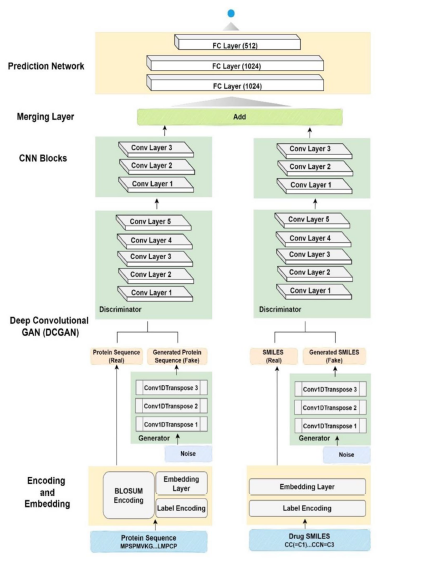
\includegraphics[width=0.96\linewidth]{presentation-figs/DCGAN-block-diagram.png}
    \end{column}

    \begin{column}{0.57\textwidth}
      \begin{block}{پنج مرحله --- شکل از پایین به بالا خوانده می‌شود}
        \footnotesize
        \begin{enumerate}\itemsep0.35ex
          \item کدگذاری و تعبیه --- \e{Label} / \e{BLOSUM} + \e{Embedding}
          \item پیش‌آموزش \e{DCGAN} --- \e{Generator} + \e{Discriminator}
          \item بلوک‌های \e{CNN} --- استخراج ویژگی
          \item لایه‌ی ادغام دو شاخه --- \e{Add}
          \item شبکه‌ی پیش‌بینی --- \e{FC 1024} $\rightarrow$ \e{512}
        \end{enumerate}
      \end{block}

      \vspace{1mm}
      \begin{alertblock}{نکته‌ی کلیدی}
        \footnotesize
        \e{GAN} اینجا \key{برای تولید دارو نیست}؛ \e{Generator} و
        \e{Discriminator} فقط برای \key{پیش‌آموزش نمایش} به کار می‌روند و
        نمایش آموخته‌شده به سر رگرسیون داده می‌شود.
      \end{alertblock}
    \end{column}
  \end{columns}
  \note{شکل را از پایین به بالا توضیح بده --- همان ترتیبی که در ستون کنارش شماره خورده است. دو شاخه‌ی چپ و راست شکل کاملاً متقارن‌اند؛ تنها تفاوت جدی، \e{BLOSUM encoding} در شاخه‌ی پروتئین است که اطلاعات تکاملی (شباهت جانشینی اسیدهای آمینه) را وارد مدل می‌کند. اگر وقت کم بود فقط بگو: کدگذاری، پیش‌آموزش تخاصمی، \e{CNN}، ادغام، رگرسیون.}
\end{frame}

%======================================================================
\section{مقاله‌ی دوم: \e{Co-VAE}}
%======================================================================

%--------------------------------------------------------------- 17 --
\begin{frame}{\e{Co-VAE}}
  \framesubtitle{نماینده‌ی شاخه‌ی \e{VAE} \ --- \ \e{Li, Zhao \& Li}, \e{IEEE TPAMI}, ۲۰۲۲}
  \vspace{3mm}
  \begin{columns}[T]
    \begin{column}{0.50\textwidth}
      \centering
      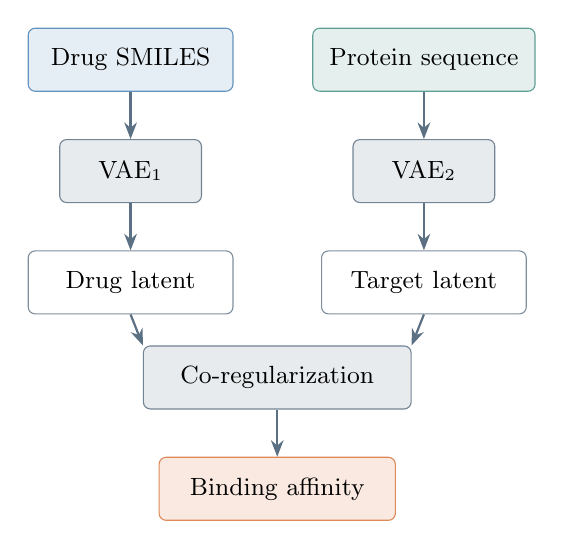
\begin{tikzpicture}[node distance=5mm,font=\footnotesize]
        \node[drug,minimum width=26mm] (d) {\e{Drug SMILES}};
        \node[model,minimum width=18mm,below=6mm of d] (v1) {\lr{$\text{VAE}_1$}};
        \node[nxn,minimum width=26mm,below=6mm of v1] (dl) {\e{Drug latent}};
        \draw[arr] (d)--(v1); \draw[arr] (v1)--(dl);

        \node[targ,minimum width=26mm,right=10mm of d] (t) {\e{Protein sequence}};
        \node[model,minimum width=18mm,below=6mm of t] (v2) {\lr{$\text{VAE}_2$}};
        \node[nxn,minimum width=26mm,below=6mm of v2] (tl) {\e{Target latent}};
        \draw[arr] (t)--(v2); \draw[arr] (v2)--(tl);

        \node[model,minimum width=34mm,below=8mm of $(dl)!0.5!(tl)$] (co) {\e{Co-regularization}};
        \node[res,minimum width=30mm,below=6mm of co] (af) {\e{Binding affinity}};
        \draw[arr] (dl.south) -- (co.north west);
        \draw[arr] (tl.south) -- (co.north east);
        \draw[arr] (co) -- (af);
      \end{tikzpicture}
    \end{column}

    \begin{column}{0.46\textwidth}
      \small
      \vspace{2mm}
      \begin{block}{ایده‌ی اصلی}
        دو \e{VAE} مجزا برای دارو و هدف، به‌همراه یک بخش
        \key{\e{co-regularization}} که فضاهای نهان را به مقدار
        \e{affinity} گره می‌زند.
      \end{block}

      \vspace{1.5mm}
      \begin{exampleblock}{چرا این مقاله مهم است}
        \footnotesize
        فضای نهان اینجا \key{احتمالاتی} است، نه یک بردار ثابت؛ و مدل فقط برای
        \e{prediction} طراحی نشده --- نویسندگان نشان می‌دهند می‌توان از آن برای
        \key{تولید داروهای جدید با هدف‌های مشابه} نیز استفاده کرد.
      \end{exampleblock}
    \end{column}
  \end{columns}
  \note{تفاوت بنیادی با مقاله‌ی قبل: آنجا نمایش با فرایند تخاصمی و در یک مرحله‌ی پیش‌آموزشِ جدا ساخته می‌شود؛ اینجا فضای نهان احتمالاتی است و بازسازی، هم‌تنظیمی و رگرسیون هم‌زمان آموزش می‌بینند. همین تقابل --- \e{Adversarial} در برابر \e{Variational} --- است که مقایسه‌ی این دو را برای پایان‌نامه ارزشمند می‌کند.}
\end{frame}

%--------------------------------------------------------------- 18 --
\begin{frame}{معماری \e{Co-VAE}}
  \framesubtitle{نمودار بلوکی مقاله --- \e{Li et al.}, \e{IEEE TPAMI}, ۲۰۲۲}
  \vspace{1mm}
  \begin{columns}[c]
    \begin{column}{0.36\textwidth}
      \centering
      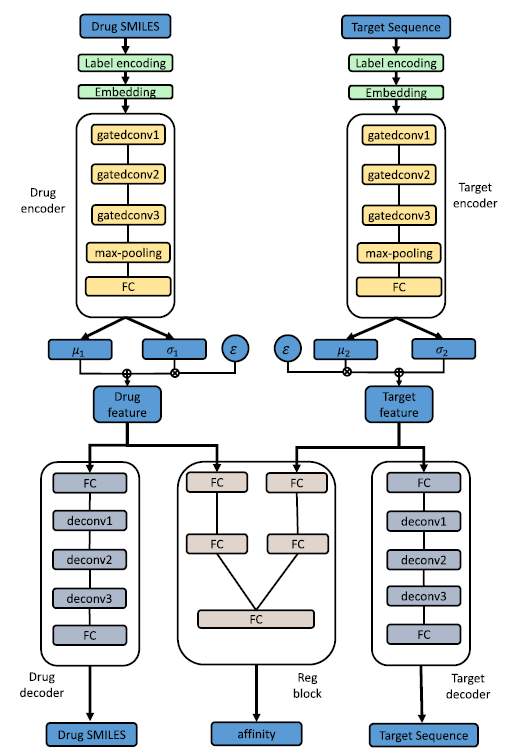
\includegraphics[width=0.94\linewidth]{presentation-figs/coVAE-block-diagram.png}
    \end{column}

    \begin{column}{0.61\textwidth}
      \begin{block}{مسیر بالا به پایین}
        \footnotesize
        \begin{enumerate}\itemsep0.3ex
          \item دو رمزگذار موازی --- \e{gatedconv}$\times$\e{3} + \e{max-pool} + \e{FC}
          \item فضای نهان --- \lr{$\mu$}، \lr{$\sigma$}، \lr{$\varepsilon$} و بازپارامتری‌سازی
        \end{enumerate}
      \end{block}

      \vspace{0.8mm}
      \begin{exampleblock}{سه سر خروجی از \e{drug} / \e{target feature}}
        \footnotesize
        \begin{itemize}\itemsep0.25ex
          \item \e{Drug decoder} --- بازسازی \e{SMILES}
          \item \E{Reg block} --- پیش‌بینی \key{\e{affinity}}
          \item \e{Target decoder} --- بازسازی توالی هدف
        \end{itemize}
      \end{exampleblock}

      \vspace{1.5mm}
      {\footnotesize\color{nxgray}
       همان دو فضای نهان هم‌زمان \key{بازسازی} و \key{رگرسیون} را تغذیه
       می‌کنند؛ همین اشتراک نقش \e{co-regularization} را بازی می‌کند.}
    \end{column}
  \end{columns}
  \note{تفاوت ساختاری مهم با \e{DCGAN-DTA}: آنجا پیش‌آموزش و رگرسیون دو مرحله‌ی جدا بودند، اینجا بازسازی و رگرسیون هم‌زمان و از یک فضای نهان مشترک آموزش می‌بینند. اگر پرسیده شد \e{co-regularization} دقیقاً چیست: یک جمله‌ی اضافه در تابع هزینه، علاوه بر دو جمله‌ی بازسازی و دو جمله‌ی \e{KL}، که فضاهای نهان دارو و هدف را طوری شکل می‌دهد که از رویشان بتوان \e{affinity} را بازیابی کرد.}
\end{frame}

%======================================================================
\section{مقایسه و خلأ پژوهشی}
%======================================================================

%--------------------------------------------------------------- 19 --
\begin{frame}{مقایسه‌ی دو رویکرد}
  \framesubtitle{\e{DCGAN-DTA} در برابر \e{Co-VAE}}
  \vspace{2mm}
  \centering
  {\footnotesize
  \rowcolors{2}{nxlight}{white}
  \begin{tabular}{p{0.22\textwidth} p{0.30\textwidth} p{0.30\textwidth}}
    \rowcolor{nxdark}
    \thd{ویژگی} & \thd{\e{DCGAN-DTA}} & \thd{\e{Co-VAE}} \\
    نوع مدل            & \e{GAN}                          & \e{VAE} \\
    ایده‌ی اصلی        & \e{Adversarial learning}         & \e{Variational learning} \\
    اجزا               & \e{Generator} + \e{Discriminator}& \e{Encoder} + \e{Decoder} \\
    فضای نهان          & تخاصمی / مولد                    & احتمالاتی \\
    نمایش دارو         & \e{SMILES}                       & \e{SMILES} \\
    نمایش هدف          & \e{Protein sequence}             & \e{Protein sequence} \\
    خروجی              & \e{Prediction}                   & \e{Prediction} + \e{co-regularization} \\
    هدف جانبی          & یادگیری نمایش                    & تولید + یادگیری نمایش \\
  \end{tabular}}

  \vspace{4mm}
  \begin{alertblock}{جمله‌ی کلیدی}
    \centering
    تفاوت اصلی این دو مقاله فقط در \e{architecture} نیست؛ آن‌ها
    \key{دو دیدگاه متفاوت} نسبت به یادگیری نمایش دارند.
  \end{alertblock}
  \note{این جدول را سطر به سطر نخوان. فقط سه سطر اول را بگو و مستقیم برو سراغ جمله‌ی پایین اسلاید، چون همان جمله ورودی بخش نوآوری است.}
\end{frame}

%--------------------------------------------------------------- 20 --
\begin{frame}{خلأ پژوهشی}
  \framesubtitle{\e{Research Gap}}
  \vspace{3mm}
  \begin{columns}[T]
    \begin{column}{0.47\textwidth}
      \begin{block}{\e{DCGAN-DTA}}
        \small تمرکز بر یادگیری نمایش مبتنی بر \e{GAN} برای \e{DTA}.
      \end{block}
      \vspace{2mm}
      \begin{exampleblock}{\e{Co-VAE}}
        \small تمرکز بر نمایش وردشی به‌همراه \e{co-regularization} برای \e{DTA}.
      \end{exampleblock}
    \end{column}

    \begin{column}{0.49\textwidth}
      \centering
      \vspace{1mm}
      \begin{tikzpicture}[font=\footnotesize,node distance=5mm]
        \node[nxn,minimum width=24mm,fill=nxblue!18,draw=nxblue!80] (a) {\e{DCGAN-DTA}};
        \node[nxn,minimum width=24mm,right=10mm of a,fill=nxteal!18,draw=nxteal!80] (b) {\e{Co-VAE}};
        \node[ghost,minimum width=40mm,below=10mm of $(a)!0.5!(b)$,draw=nxred!70,dashed,text=nxred]
          (g) {\fa{پروتکل آزمایشی مشترک؟}};
        \draw[arrd,draw=nxred!70] (a) -- (g);
        \draw[arrd,draw=nxred!70] (b) -- (g);
      \end{tikzpicture}
    \end{column}
  \end{columns}

  \vspace{4mm}
  \begin{alertblock}{خلأ}
    \centering
    مقایسه‌ی \key{مستقیم و کنترل‌شده}ی این دو پارادایم تحت یک
    \e{experimental protocol} مشترک، مسئله‌ای است که در این پایان‌نامه بررسی می‌شود.
  \end{alertblock}
  \note{اینجا محتاط باش و ادعای بزرگ نکن. نگو «هیچ‌کس این کار را نکرده»؛ بگو «تا جایی که بررسی کرده‌ام، مقایسه‌ی کنترل‌شده‌ی این دو خانواده تحت یک پروتکل یکسان کمتر انجام شده است». این جمله قابل دفاع‌تر است.}
\end{frame}

%======================================================================
\section{نوآوری پیشنهادی}
%======================================================================

%--------------------------------------------------------------- 21 --
\begin{frame}{نوآوری‌های پیشنهادی}
  \framesubtitle{چهار محور اصلی پایان‌نامه}
  \vspace{3mm}
  \begin{columns}[T]
    \begin{column}{0.48\textwidth}
      \small
      \begin{block}{۱. مقایسه‌ی دو پارادایم مولد}
        \e{Adversarial learning} در برابر \e{Variational learning}
        برای مسئله‌ی \e{DTA}.
      \end{block}

      \vspace{1mm}
      \begin{block}{۲. پروتکل آزمایشی یکسان}
        مجموعه‌داده، \e{preprocessing}، نمایش‌ها، \e{split}، معیارها و
        \e{seed}های کنترل‌شده --- تا تفاوت عملکرد واقعاً به
        \e{architecture} نسبت داده شود.
      \end{block}
    \end{column}

    \begin{column}{0.48\textwidth}
      \small
      \begin{block}{۳. بررسی \e{generalization}}
        مقایسه در دو شرایط \e{warm-start} و \e{cold-start}؛ عملکرد روی
        \e{random split} لزوماً توان پیش‌بینی برای داروها و هدف‌های
        واقعاً جدید را نشان نمی‌دهد.
      \end{block}

      \vspace{1mm}
      \begin{block}{۴. تحلیل فراتر از دقت}
        علاوه بر \e{performance}: \e{generalization}،
        \e{training stability}، \e{computational cost} و
        \e{data efficiency}.
      \end{block}
    \end{column}
  \end{columns}

  \vspace{3mm}
  \centering
  {\footnotesize\color{nxgray}
   \e{DCGAN-DTA} نیز همین مسئله را با \e{warm-start} و \e{cold-start} فیزیکوشیمیایی مورد توجه قرار داده است.}
  \note{مهم‌ترین اسلاید دفاع از نوآوری. اگر استاد گفت «این فقط مقایسه است، نوآوری نیست»، پاسخ آماده داشته باش: نوآوری در طراحی پروتکل کنترل‌شده و در تحلیل چندبعدی (نه صرفاً عدد دقت) است، و خروجی آن یک راهنمای انتخاب مدل برای این حوزه است.}
\end{frame}

%--------------------------------------------------------------- 22 --
\begin{frame}{سؤال اصلی پژوهش}
  \framesubtitle{پرسش اصلی و پرسش‌های فرعی}
  \vspace{2mm}
  \begin{alertblock}{پرسش اصلی}
    \centering
    آیا نوع روش یادگیری مولد --- \key{تخاصمی} یا \key{وردشی} --- می‌تواند بر
    کیفیت یادگیری نمایش و عملکرد پیش‌بینی قدرت اتصال در مسئله‌ی \e{DTA}
    تأثیر معناداری داشته باشد؟
  \end{alertblock}

  \vspace{1.5mm}
  \begin{block}{پرسش‌های فرعی}
    \footnotesize
    \begin{enumerate}\itemsep0.35ex
      \item کدام روش در \e{warm-start} عملکرد بهتری دارد؟
      \item کدام روش در \e{cold-start} بهتر \e{generalize} می‌کند؟
      \item حساسیت هر مدل نسبت به حجم داده چقدر است؟
      \item کدام مدل از نظر \e{computational cost} مناسب‌تر است؟
      \item آیا برتری مشاهده‌شده ناشی از \e{architecture} است یا از
            \e{dataset} / \e{split} / \e{preprocessing}؟
    \end{enumerate}
  \end{block}
  \note{ارائه باید با همین اسلاید به اوج برسد. پرسش پنجم مهم‌ترین است و نشان می‌دهد به اعتبار درونی آزمایش فکر کرده‌ای؛ روی همان یک مکث کوتاه کن.}
\end{frame}

%--------------------------------------------------------------- 23 --
\begin{frame}{روایت کلی ارائه}
  \framesubtitle{جمع‌بندی بصری مسیر ارائه}
  \vspace{3mm}
  \centering
  % سه سطر: صورت‌مسئله، مسیر روش‌ها، و جمع‌بندی به نوآوری
  \begin{tikzpicture}[x=1mm,y=1mm,font=\scriptsize]
    % --- row 1: the problem ---
    \node[ghost,minimum width=20mm] (dti) at (14,24) {\e{DTI}};
    \node[ghost,minimum width=20mm] (dta) at (44,24) {\e{DTA}};
    \node[nxn,minimum width=30mm]   (aff) at (84,24) {\e{Binding affinity}};
    \draw[arr] (dti)--(dta); \draw[arr] (dta)--(aff);
    % برچسب‌ها بالای سطر اول تا مسیر اتصال به سطر دوم آزاد بماند
    \node[lbl,text width=22mm,align=center] at (14,32) {\fa{هست یا نیست؟}};
    \node[lbl,text width=22mm,align=center] at (44,32) {\fa{چقدر قوی؟}};
    \node[lbl,text width=30mm,align=center] at (84,32) {\e{Kd} / \e{Ki} / \e{IC50}};

    % --- row 2: how the field got here ---
    \node[ghost,minimum width=18mm] (cls) at (11,4)  {\fa{کلاسیک}};
    \node[ghost,minimum width=13mm] (mlx) at (33,4)  {\e{ML}};
    \node[model,minimum width=13mm] (dlx) at (53,4)  {\e{DL}};
    \node[model,minimum width=32mm] (rep) at (87,4)  {\e{Representation learning}};
    \node[res,minimum width=18mm]   (gen) at (117,4) {\fa{مدل‌های مولد}};
    \draw[arr] (cls)--(mlx); \draw[arr] (mlx)--(dlx);
    \draw[arr] (dlx)--(rep); \draw[arr] (rep)--(gen);
    \draw[arr] (aff.south) -- ++(0,-6) -| (cls.north);

    % --- row 3: the two papers, the comparison, the contribution ---
    \node[nxn,minimum width=24mm,fill=nxblue!18,draw=nxblue!80] (g1) at (14,-16) {\e{DCGAN-DTA}};
    \node[nxn,minimum width=18mm,fill=nxteal!18,draw=nxteal!80] (g2) at (42,-16) {\e{Co-VAE}};
    \node[nxn,minimum width=30mm,draw=nxred!70,fill=nxred!8]    (cmp) at (80,-16) {\fa{مقایسه‌ی کنترل‌شده}};
    \node[res,minimum width=26mm,fill=nxaccent!30,draw=nxaccent] (nov) at (115,-16) {\fa{نوآوری پایان‌نامه}};
    \draw[arr] (g1)--(g2);
    \draw[arr] (g2)--(cmp);
    \draw[arr] (cmp)--(nov);
    \draw[arr] (gen.south) -- ++(0,-5) -| (g1.north);
  \end{tikzpicture}
  \note{این اسلاید جمع‌بندی بصری است. می‌توانی آن را ۱۵ ثانیه‌ای رد کنی یا اگر جلسه طولانی شد مستقیم از اسلاید ۲۲ به اسلاید پرسش‌ها بروی.}
\end{frame}

%--------------------------------------------------------------- 24 --
\begin{frame}{مراجع اصلی}
  \framesubtitle{منابع کلیدی این ارائه}
  \vspace{4mm}
  \small
  % هر مرجع یک بازه‌ی کامل چپ‌به‌راست است تا ترتیب اجزای استناد به‌هم نریزد
  \vspace{-2mm}
  \begin{enumerate}\footnotesize\itemsep0.35ex
    \item \lr{Wang et al., \textit{A unified survey on drug--target interaction
          and binding affinity prediction}, Biotechnology Advances, 2026.}
    \item \lr{Pahikkala et al., \textit{Toward more realistic drug--target
          interaction predictions} (KronRLS), Brief.\ Bioinform., 2015.}
    \item \lr{He et al., \textit{SimBoost: a read-across approach using gradient
          boosting machines}, J.\ Cheminformatics, 2017.}
    \item \lr{Öztürk et al., \textit{DeepDTA: deep drug--target binding affinity
          prediction}, Bioinformatics, 2018.}
    \item \lr{Öztürk et al., \textit{WideDTA: prediction of drug--target binding
          affinity}, arXiv, 2019.}
    \item \lr{Nguyen et al., \textit{GraphDTA: predicting drug--target binding
          affinity with graph neural networks}, Bioinformatics, 2021.}
    \item \lr{Li et al., \textit{Co-VAE: Drug--Target Binding Affinity Prediction
          by Co-Regularized Variational Autoencoders}, IEEE TPAMI, 2022.}
    \item \lr{Kalemati et al., \textit{DCGAN-DTA: Predicting drug--target binding
          affinity with deep convolutional GANs}, BMC Genomics, 2024.}
  \end{enumerate}

  \vspace{4mm}
  {\footnotesize\color{nxgray}
   فهرست کامل مراجع در متن پایان‌نامه ارائه شده است.}
  \note{این اسلاید فقط برای مستند بودن است؛ روی آن توقف نکن مگر استاد سؤال کند.}
\end{frame}

%--------------------------------------------------------------- 25 --
\begin{frame}[plain,noframenumbering]
  \vfill
  \begin{center}
    {\lr{\textcolor{nxaccent}{\rule{28mm}{1.6pt}}}}\\[6mm]
    {\Large\bfseries\color{nxdark} با تشکر از توجه شما}\\[5mm]
    {\large\color{nxgray} پرسش‌ها و پیشنهادها}\\[8mm]
    {\small محسن کاشفی کیا \quad$\cdot$\quad استاد راهنما: دکتر سایه میرزایی}
  \end{center}
  \vfill
  \note{آماده باش برای این سه سؤال: (۱) چرا همین دو مقاله را انتخاب کردی؟ (۲) داده و منابع محاسباتی را چطور تأمین می‌کنی؟ (۳) اگر نتیجه این شد که تفاوت معنادار نیست، دستاورد پایان‌نامه چیست؟ برای سؤال سوم پاسخ بده: نتیجه‌ی منفی هم یافته است، چون نشان می‌دهد تفاوت گزارش‌شده در مقالات ناشی از پروتکل بوده نه معماری.}
\end{frame}

\end{document}
"
%======================================================================
\documentclass[11pt,aspectratio=169,xcolor=table]{beamer}

\usetheme{default}
\usecolortheme{default}
\setbeamertemplate{navigation symbols}{}

\usepackage{amsmath,amssymb}
\usepackage{xcolor}
\usepackage{tikz}
\usetikzlibrary{arrows.meta,positioning,shapes.geometric,fit,backgrounds,calc,decorations.pathreplacing}
\usepackage{array}

%------------------------------- palette ------------------------------
\definecolor{nxdark}{HTML}{16334F}
\definecolor{nxblue}{HTML}{2F6FA8}
\definecolor{nxteal}{HTML}{2A7F6F}
\definecolor{nxaccent}{HTML}{D9743B}
\definecolor{nxred}{HTML}{B5453A}
\definecolor{nxgray}{HTML}{6B7785}
\definecolor{nxlight}{HTML}{EDF2F7}

%------------------------------- fonts --------------------------------
\usepackage{xepersian}
\settextfont[Scale=1.0]{XB Zar}
\setdigitfont[Scale=1.0]{XB Zar}
\setlatintextfont[Scale=0.92]{Cambria}

% سازگاری: وصله‌ی bidi برای jadval به ماکرویی ارجاع می‌دهد که از نسخه‌های
% جدید array.sty حذف شده است.
\providecommand\UseMathForPositioningText{}

%------------------------------ beamer look ---------------------------
\setbeamercolor{structure}{fg=nxdark}
\setbeamercolor{frametitle}{fg=white,bg=nxdark}
\setbeamercolor{framesubtitle}{fg=nxgray}
\setbeamercolor{footline}{fg=nxgray}
\setbeamercolor{normal text}{fg=nxdark!95}
\setbeamercolor{itemize item}{fg=nxaccent}
\setbeamercolor{itemize subitem}{fg=nxblue}
\setbeamercolor{block title}{fg=white,bg=nxblue}
\setbeamercolor{block body}{fg=nxdark,bg=nxblue!8}
\setbeamercolor{block title alerted}{fg=white,bg=nxaccent}
\setbeamercolor{block body alerted}{fg=nxdark,bg=nxaccent!10}
\setbeamercolor{block title example}{fg=white,bg=nxteal}
\setbeamercolor{block body example}{fg=nxdark,bg=nxteal!8}

\setbeamerfont{frametitle}{size=\large,series=\bfseries}
\setbeamerfont{framesubtitle}{size=\small}
\setbeamerfont{footline}{size=\scriptsize}
\setbeamerfont{block title}{size=\small,series=\bfseries}
\setbeamerfont{block body}{size=\small}

\setbeamertemplate{itemize item}{\raisebox{0.15ex}{\tiny$\blacktriangleleft$}}
\setbeamertemplate{itemize subitem}{\raisebox{0.15ex}{\tiny$\blacktriangleleft$}}
% قالب rounded بیمر با bidi به‌هم می‌ریزد؛ قالب ساده پایدار است.
\setbeamertemplate{blocks}[default]

% ---- frame title: full-width bar + accent rule ----
\definecolor{nxsub}{HTML}{A9BDD1}
\setbeamercolor{nxrule}{bg=nxaccent,fg=nxaccent}
\setbeamercolor{framesubtitle}{fg=nxsub,bg=nxdark}

% نکته‌ی مهم درباره‌ی bidi: در قالب‌های بیمر، فقط نخستین beamercolorbox رسم
% می‌شود و \rule داخل متن راست‌به‌چپ رنگ خود را از دست می‌دهد (سیاه می‌شود).
% بنابراین همه‌ی تزئینات (خط نارنجی سربرگ و نوار پیشرفت پاورقی) با tikz در
% قالب background canvas کشیده می‌شوند و سربرگ همیشه دو سطری است تا ارتفاع
% آن ثابت بماند.
\makeatletter
\setbeamertemplate{frametitle}{%
  \begin{beamercolorbox}[wd=\paperwidth,leftskip=1em,rightskip=1em]{frametitle}%
    \vspace{1.1ex}%
    {\usebeamerfont{frametitle}\insertframetitle}\\[0.1ex]%
    % هر اسلاید باید \framesubtitle داشته باشد تا ارتفاع سربرگ ثابت بماند و
    % خط نارنجیِ کشیده‌شده در background canvas دقیقاً زیر نوار بنشیند.
    {\usebeamerfont{framesubtitle}\usebeamercolor[fg]{framesubtitle}%
     \insertframesubtitle}%
    \vspace{1.0ex}%
  \end{beamercolorbox}%
}
\makeatother

% ---- footer: section name + frame number (chrome drawn in background) ----
\setbeamertemplate{footline}{%
  \begin{beamercolorbox}[wd=\paperwidth,ht=2.4ex,dp=1.4ex,leftskip=1em,rightskip=1em]{footline}%
    \usebeamerfont{footline}%
    \insertsectionhead\hfill\insertframenumber\,/\,\inserttotalframenumber%
  \end{beamercolorbox}%
}

% ---- all decorative chrome, drawn with tikz so bidi cannot swallow it ----
\newlength{\nxprogw}
\newlength{\nxhdrh}
\setlength{\nxhdrh}{37.2pt}    % ارتفاع نوار سربرگ (دو سطری، ثابت)
\makeatletter
\setbeamertemplate{background canvas}{%
  \setlength{\nxprogw}{\dimexpr\paperwidth/\inserttotalframenumber*\insertframenumber\relax}%
  \begin{tikzpicture}[overlay,remember picture]
    \fill[white] (current page.south west) rectangle (current page.north east);
    \ifbeamer@plainframe\else
      \fill[nxaccent] (current page.north west) ++(0,-\nxhdrh)
                      rectangle ++(\paperwidth,-1.2pt);
    \fi
    \fill[nxdark!12] (current page.south west) rectangle ++(\paperwidth,1pt);
    \fill[nxaccent]  (current page.south east) ++(-\nxprogw,0)
                     rectangle ++(\nxprogw,1pt);
  \end{tikzpicture}%
}
\makeatother

% ---- notes ----
\ifdefined\notesmode
  \setbeameroption{show only notes}
\else
  \setbeameroption{hide notes}
\fi
\setbeamerfont{note page}{size=\small}

%------------------------------ tikz styles ---------------------------
\tikzset{
  nxn/.style   ={draw=nxdark!55, rounded corners=2.5pt, fill=white,
                 inner xsep=6pt, inner ysep=4pt, minimum height=8mm,
                 font=\small, align=center},
  drug/.style  ={nxn, fill=nxblue!12,   draw=nxblue!75},
  targ/.style  ={nxn, fill=nxteal!12,   draw=nxteal!75},
  model/.style ={nxn, fill=nxdark!10,   draw=nxdark!60},
  res/.style   ={nxn, fill=nxaccent!16, draw=nxaccent!85},
  ghost/.style ={nxn, fill=nxlight,     draw=nxdark!25, text=nxgray},
  lbl/.style   ={font=\scriptsize, text=nxgray, inner sep=2pt},
  arr/.style   ={-{Stealth[length=2.1mm,width=1.6mm]}, draw=nxdark!70, thick},
  arrd/.style  ={arr, dashed},
  flat/.style  ={draw=none, fill=none, font=\small, align=center},
}

%-------------------------- small helper macros -----------------------
\newcommand{\E}[1]{\lr{\textbf{#1}}}
\newcommand{\e}[1]{\lr{#1}}
% متن فارسی داخل گره‌های tikz به صورت پاراگراف چپ‌به‌راست چیده می‌شود و ترتیب
% واژه‌ها برعکس می‌شود؛ \fa کل متن گره را در یک بازه‌ی راست‌به‌چپ قرار می‌دهد.
% توجه: داخل \fa نباید \\ بیاید — هر سطر را جداگانه باید پیچید.
\newcommand{\fa}[1]{\RLE{#1}}
% ریاضیِ نمایشی: \[...\] در ستون راست‌به‌چپ سرریز می‌کند و دیده نمی‌شود؛
% همچنین \lr باعث می‌شود ارقام داخل فرمول لاتین بمانند نه فارسی.
\newcommand{\disp}[1]{\begin{center}\lr{$\displaystyle #1$}\end{center}}
\newcommand{\key}[1]{\textcolor{nxaccent}{\textbf{#1}}}
\newcommand{\thd}[1]{\textcolor{white}{\textbf{#1}}}

% section divider
\AtBeginSection[]{%
  \begin{frame}[plain,noframenumbering]
    \vfill
    \begin{center}
      {\lr{\textcolor{nxaccent}{\rule{22mm}{1.6pt}}}}\\[4mm]
      {\usebeamerfont{frametitle}\Large\color{nxdark}\insertsectionhead}\\[3mm]
      {\lr{\textcolor{nxdark!20}{\rule{60mm}{0.7pt}}}}
    \end{center}
    \vfill
  \end{frame}
}

\begin{document}

%======================================================================
% TITLE
%======================================================================
\begin{frame}[plain,noframenumbering]
  \vspace{-3mm}
  \hbox to\textwidth{%
    
\includegraphics[height=11mm]{First-Pages/TehUni.png}\hfill
    
\includegraphics[height=11mm]{First-Pages/Eng.png}}

  \vspace{-6mm}
  \begin{center}
    {\footnotesize دانشگاه تهران — پردیس دانشکده‌های فنی}\\[0.4mm]
    {\footnotesize دانشکده علوم مهندسی — گروه الگوریتم‌ها و محاسبات}

    \vspace{3mm}
    {\lr{\textcolor{nxaccent}{\rule{30mm}{1.2pt}}}}

    \vspace{2.5mm}
    {\large\bfseries\color{nxdark} پیش‌بینی قدرت اتصال دارو--هدف\\[1mm]
     با مدل‌های مولد}\\[2mm]
    {\small\color{nxgray} مقایسه‌ی کنترل‌شده‌ی یادگیری تخاصمی و یادگیری وردشی}\\[0.6mm]
    {\scriptsize\color{nxgray}\e{Adversarial vs.\ Variational Representation Learning for Drug--Target Affinity}}

    \vspace{3mm}
    {\lr{\textcolor{nxdark!20}{\rule{70mm}{0.5pt}}}}\\[2mm]

    {\footnotesize ارائه‌دهنده: \textbf{محسن کاشفی کیا}}\\[0.8mm]
    {\footnotesize استاد راهنما: \textbf{دکتر سایه میرزایی}}\\[2mm]
    {\scriptsize\color{nxgray} گزارش پیشرفت پایان‌نامه کارشناسی ارشد \quad$\cdot$\quad شهریور ۱۴۰۵}
  \end{center}
  \note{سلام و تشکر از استاد. در یک جمله بگو: «هدف این جلسه این است که مسیر رسیدن از صورت‌مسئله تا نوآوری پیشنهادی پایان‌نامه را مرور کنیم.» زمان پیشنهادی کل ارائه: ۲۰ تا ۲۵ دقیقه.}
\end{frame}

%======================================================================
% OUTLINE
%======================================================================
\begin{frame}{فهرست مطالب}
  \framesubtitle{مسیر ارائه در یک نگاه}
  \vspace{3mm}
  \begin{columns}[T]
    \begin{column}{0.52\textwidth}
      \small
      \begin{enumerate}
        \item تعریف مسئله: از \e{DTI} تا \e{DTA}
        \item معیارهای کمی قدرت اتصال
        \item درخت تکاملی روش‌ها: از \e{KronRLS} تا مدل‌های بنیادی
        \item جایگاه پایان‌نامه در این درخت
        \item مقاله‌ی اول: \e{DCGAN-DTA} --- شاخه‌ی \e{GAN}
        \item مقاله‌ی دوم: \e{Co-VAE} --- شاخه‌ی \e{VAE}
        \item خلأ پژوهشی و نوآوری پیشنهادی
      \end{enumerate}
    \end{column}
    \begin{column}{0.44\textwidth}
      \begin{tikzpicture}[node distance=4.5mm,every node/.style={font=\scriptsize}]
        \node[ghost,minimum width=32mm] (a) {\fa{\e{DTI} — آیا برهم‌کنش هست؟}};
        \node[ghost,minimum width=32mm,below=of a] (b) {\fa{\e{DTA} — چقدر قوی است؟}};
        \node[model,minimum width=32mm,below=of b] (c) {\fa{مسیر پژوهشی تا مدل‌های مولد}};
        \node[res,minimum width=32mm,below=of c] (d) {\fa{نوآوری پیشنهادی}};
        \draw[arr] (a)--(b); \draw[arr] (b)--(c); \draw[arr] (c)--(d);
      \end{tikzpicture}
    \end{column}
  \end{columns}
  \note{این اسلاید نقشه‌ی راه است. یک جمله بگو: «ارائه از صورت‌مسئله شروع می‌شود، به دو مقاله‌ی مرجع می‌رسد و با سؤال پژوهشی پایان‌نامه تمام می‌شود.» روی آن معطل نشو.}
\end{frame}

%======================================================================
\section{تعریف مسئله}
%======================================================================

%---------------------------------------------------------------- 1 --
\begin{frame}{برهم‌کنش دارو--هدف چیست؟}
  \framesubtitle{\e{Drug--Target Interaction (DTI)}}
  \vspace{2mm}
  \begin{columns}[T]
    \begin{column}{0.46\textwidth}
      \small
      در فرآیند \e{drug discovery}، یکی از مسائل پایه شناسایی ارتباط میان
      \key{دارو} و \key{پروتئین هدف} است.

      \vspace{2mm}
      \begin{block}{پرسش \e{DTI}}
        آیا یک دارو می‌تواند با یک پروتئین هدف برهم‌کنش داشته باشد یا خیر؟
      \end{block}

      \vspace{1mm}
      {\footnotesize\color{nxgray}
       خروجی مسئله \key{دودویی} است: بله / خیر.}
    \end{column}
    \begin{column}{0.50\textwidth}
      \centering
      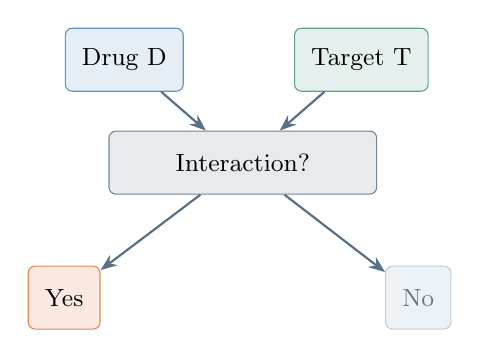
\begin{tikzpicture}[node distance=7mm]
        \node[drug]                       (d) {\e{Drug D}};
        \node[targ, right=14mm of d]      (t) {\e{Target T}};
        \node[model, below=9mm of $(d)!0.5!(t)$, minimum width=34mm] (i) {\e{Interaction?}};
        \node[res,  below left=9mm and 1mm of i]  (y) {\e{Yes}};
        \node[ghost,below right=9mm and 1mm of i] (n) {\e{No}};
        \draw[arr] (d) -- (i);
        \draw[arr] (t) -- (i);
        \draw[arr] (i) -- (y);
        \draw[arr] (i) -- (n);
      \end{tikzpicture}
    \end{column}
  \end{columns}
  \note{\e{DTI} را به عنوان مسئله‌ی پایه معرفی کن: «اگر بخواهیم فضای جستجوی \e{drug discovery} را کوچک کنیم، اولین سؤال این است که از میان تعداد زیادی دارو و پروتئین، کدام جفت‌ها احتمالاً با هم برهم‌کنش دارند.» مقاله‌ی \e{Co-VAE} هم مقدمه‌اش را از همین نقطه شروع می‌کند.}
\end{frame}

%---------------------------------------------------------------- 2 --
\begin{frame}{از تشخیص برهم‌کنش به اندازه‌گیری قدرت آن}
  \framesubtitle{چرا پاسخ بله/خیر کافی نیست؟}
  \vspace{1mm}
  \centering
  \begin{tikzpicture}[x=1mm,y=1mm,font=\footnotesize]
    % --- inputs ---
    \node[drug] (d1) at (0,7)   {\e{Drug A}};
    \node[drug] (d2) at (0,-7)  {\e{Drug B}};
    \node[targ] (tx) at (28,0)  {\e{Target X}};
    \draw[arr] (d1) -- (tx);
    \draw[arr] (d2) -- (tx);

    % --- DTI column ---
    \node[lbl,text=nxdark,font=\scriptsize\bfseries] at (60,17) {\fa{دیدِ \e{DTI}}};
    \node[res,minimum width=26mm]   (y1) at (60,7)  {\e{Yes}};
    \node[res,minimum width=26mm]   (y2) at (60,-7) {\e{Yes}};
    \draw[arr] (tx) -- (y1);
    \draw[arr] (tx) -- (y2);
    \node[lbl,text width=32mm,align=center] at (60,-17) {\fa{هر دو یکسان دیده می‌شوند}};

    % --- divider ---
    \draw[nxdark!20,thick] (80,20) -- (80,-20);

    % --- DTA column ---
    \node[lbl,text=nxdark,font=\scriptsize\bfseries] at (104,17) {\fa{دیدِ \e{DTA}}};
    \node[nxn,minimum width=28mm,fill=nxred!18,draw=nxred!80] (s1) at (104,7)  {\e{Strong binding}};
    \node[ghost,minimum width=28mm]                           (s2) at (104,-7) {\e{Weak binding}};
    \draw[arr,draw=nxdark!35] (y1) -- (s1);
    \draw[arr,draw=nxdark!35] (y2) -- (s2);
    \node[lbl,text width=34mm,align=center] at (104,-17) {\fa{دو دارو از هم تفکیک می‌شوند}};
  \end{tikzpicture}

  \vspace{2mm}
  \begin{alertblock}{پرسش دقیق‌تر}
    \centering قدرت اتصال دارو به هدف \key{چقدر} است؟ \quad$\Rightarrow$\quad مسئله‌ی \E{Drug--Target Binding Affinity (DTA)}
  \end{alertblock}
  \note{نکته‌ی کلیدی: دو دارو می‌توانند هر دو با یک \e{target} برهم‌کنش داشته باشند، ولی یکی اتصال بسیار قوی و دیگری اتصال ضعیف. \e{DTI} این تفاوت را نمی‌بیند. اینجا گذار از مسئله‌ی دسته‌بندی به مسئله‌ی رگرسیون اتفاق می‌افتد.}
\end{frame}

%---------------------------------------------------------------- 3 --
\begin{frame}{چرا \e{DTA}؟}
  \framesubtitle{اطلاعات کمی در برابر اطلاعات دودویی}
  \vspace{2mm}
  \centering
  {\small
  \rowcolors{2}{nxlight}{white}
  \begin{tabular}{p{0.34\textwidth} p{0.34\textwidth}}
    \rowcolor{nxdark}
    \thd{\e{DTI}} & \thd{\e{DTA}} \\
    آیا برهم‌کنش وجود دارد؟ & برهم‌کنش چقدر قوی است؟ \\
    خروجی دودویی (\e{binary})   & خروجی پیوسته (\e{continuous}) \\
    بله / خیر                & مقدار عددی \e{affinity} \\
    مناسب غربالگری اولیه     & مناسب رتبه‌بندی و اولویت‌دهی \\
  \end{tabular}}

  \vspace{4mm}
  \begin{columns}[c]
    \begin{column}{0.55\textwidth}
      \begin{exampleblock}{جمله‌ی کلیدی}
        \e{DTA} علاوه بر \key{وجود} برهم‌کنش، \key{شدت} آن را نیز مشخص می‌کند و
        بنابراین اطلاعات غنی‌تری در اختیار می‌گذارد.
      \end{exampleblock}
    \end{column}
    \begin{column}{0.42\textwidth}
      {\footnotesize\color{nxgray}
       \textbf{دقت در بیان:} نگوییم «\e{DTA} همیشه بهتر از \e{DTI} است»؛
       این‌ها دو صورت‌بندی متفاوت از مسئله‌اند. بگوییم برای \emph{هدف این پژوهش}،
       اطلاعات کمی \e{affinity} ارزشمندتر است.}
    \end{column}
  \end{columns}
  \note{حتماً تأکید کن که \e{DTA} و \e{DTI} دو \e{formulation} متفاوت‌اند، نه اینکه یکی مطلقاً بهتر از دیگری باشد. این جمله از نظر علمی قابل دفاع‌تر است و معمولاً همین‌جا سؤال پرسیده می‌شود. \e{Co-VAE} هم پیش‌بینی \e{affinity} را چالش‌برانگیزتر از تشخیص \e{interaction} می‌داند.}
\end{frame}

%---------------------------------------------------------------- 4 --
\begin{frame}{قدرت اتصال چگونه اندازه‌گیری می‌شود؟}
  \framesubtitle{نقشه‌ی معیارهای متداول}
  \vspace{4mm}
  \centering
  \begin{tikzpicture}[node distance=5mm]
    \node[model,minimum width=30mm] (root) {\fa{اندازه‌گیری \e{Affinity}}};

    \node[targ,minimum width=44mm,below right=12mm and 2mm of root] (ba) {\e{Binding affinity}\\[-1mm] \fa{{\scriptsize قدرت اتصال ترمودینامیکی}}};
    \node[res, minimum width=40mm,below left=12mm and 2mm of root]  (po) {\e{Potency / inhibition}\\[-1mm] \fa{{\scriptsize اثر عملکردی در آزمایش}}};

    \node[nxn,below left=10mm and -2mm of ba]  (kd) {\e{Kd} \ / \ \e{pKd}};
    \node[nxn,below right=10mm and -2mm of ba] (ki) {\e{Ki} \ / \ \e{pKi}};
    \node[nxn,below=10mm of po]                (ic) {\e{IC50}};

    \draw[arr] (root) -- (ba);
    \draw[arr] (root) -- (po);
    \draw[arr] (ba) -- (kd);
    \draw[arr] (ba) -- (ki);
    \draw[arr] (po) -- (ic);
  \end{tikzpicture}

  \vspace{3mm}
  {\footnotesize\color{nxgray}
   در اسلایدهای بعد هر معیار جداگانه تعریف می‌شود؛ تمایز ستون راست و چپ نکته‌ی اصلی این بخش است.}
  \note{این اسلاید «نقشه» است. فقط بگو چهار پنج اصطلاح داریم و مهم‌ترین نکته این است که \e{Kd} و \e{Ki} معیار \e{binding affinity} هستند ولی \e{IC50} معیار \e{potency} عملکردی است. جزئیات را در اسلایدهای بعد باز می‌کنی.}
\end{frame}

%---------------------------------------------------------------- 5 --
\begin{frame}{\e{Kd} و \e{pKd}}
  \framesubtitle{\e{Equilibrium Dissociation Constant}}
  \vspace{1mm}
  \begin{columns}[T]
    \begin{column}{0.50\textwidth}
      \small
      \begin{block}{تعریف مفهومی}
        \e{Kd} غلظتی از \e{ligand} است که در شرایط تعادل، تقریباً \key{نیمی} از
        \e{target}ها را در حالت \e{bound} قرار می‌دهد.
      \end{block}

      \vspace{-1mm}
      \disp{K_d \;=\; \frac{[D]\,[T]}{[DT]}}

      \vspace{-3mm}
      {\footnotesize
      \e{D}: داروی آزاد \quad $\cdot$ \quad \e{T}: هدف آزاد \quad $\cdot$ \quad \e{DT}: کمپلکس دارو--هدف}

      \vspace{2mm}
      \begin{alertblock}{مقیاس لگاریتمی}
        \vspace{-3mm}
        \disp{pK_d \;=\; -\log_{10}\!\big(K_d\,[M]\big)}
        \vspace{-3mm}
        \centering اگر \lr{$K_d = 10^{-9}\,M$} آنگاه \lr{$pK_d = 9$}
      \end{alertblock}
    \end{column}

    \begin{column}{0.46\textwidth}
      \centering
      \vspace{3mm}
      % مقیاس به‌صورت راست‌به‌چپ خوانده می‌شود: سمت راست = اتصال قوی
      \begin{tikzpicture}
        \shade[left color=nxlight,right color=nxred!55] (0,0) rectangle (6.4,0.55);
        \draw[nxdark!35] (0,0) rectangle (6.4,0.55);
        \node[lbl,below] at (5.8,0) {\fa{\e{Kd} کوچک}};
        \node[lbl,below] at (0.6,0) {\fa{\e{Kd} بزرگ}};
        \node[lbl,above,text=nxdark,font=\scriptsize\bfseries] at (5.4,0.55) {\fa{اتصال قوی}};
        \node[lbl,above,text=nxdark,font=\scriptsize\bfseries] at (1.0,0.55) {\fa{اتصال ضعیف}};

        \node[drug,minimum width=24mm,below=11mm of {(5.4,0)},font=\scriptsize] (a)
          {\e{Drug A}\\[-1mm]{\scriptsize\e{Kd = 1 nM}}};
        \node[ghost,minimum width=24mm,below=11mm of {(1.0,0)},font=\scriptsize] (b)
          {\e{Drug B}\\[-1mm]{\scriptsize\e{Kd = 100 nM}}};
      \end{tikzpicture}

      \vspace{6mm}
      {\small\color{nxdark}
       \lr{$K_d \downarrow$} \quad$\Longrightarrow$\quad \e{affinity} \lr{$\uparrow$} \quad$\Longrightarrow$\quad \lr{$pK_d \uparrow$}}
    \end{column}
  \end{columns}
  \note{نکته‌ای که معمولاً پرسیده می‌شود: چرا لگاریتم می‌گیریم؟ چون مقادیر \e{Kd} در بازه‌ای بسیار وسیع و بسیار کوچک (نانومولار تا میکرومولار) پخش‌اند و مقیاس لگاریتمی هم عددها را قابل‌مدیریت می‌کند و هم برای رگرسیون مناسب‌تر است. جهت را اشتباه نگو: \e{Kd} کمتر یعنی \e{affinity} بیشتر.}
\end{frame}

%---------------------------------------------------------------- 6 --
\begin{frame}{\e{Ki} و \e{pKi}}
  \framesubtitle{\e{Inhibition Constant}}
  \vspace{2mm}
  \begin{columns}[T]
    \begin{column}{0.50\textwidth}
      \small
      \begin{block}{تعریف}
        \e{Ki} معیاری برای بیان \e{affinity} یک \key{مهارکننده} (\e{inhibitor})
        نسبت به \e{target} یا آنزیم است.
      \end{block}

      \vspace{1mm}
      هرچه \e{Ki} کوچک‌تر باشد، \e{inhibitor} تمایل بیشتری به اتصال مؤثر
      به \e{target} دارد.

      \vspace{-1mm}
      \disp{pK_i \;=\; -\log_{10}\!\big(K_i\,[M]\big)}

      \vspace{-2mm}
      \centering
      {\small \lr{$K_i \downarrow$} \quad$\Longrightarrow$\quad \lr{$pK_i \uparrow$} \quad$\Longrightarrow$\quad \e{affinity} \lr{$\uparrow$}}
    \end{column}

    \begin{column}{0.46\textwidth}
      \vspace{2mm}
      \begin{alertblock}{\e{Ki} و \e{Kd} یکی نیستند}
        \small
        \begin{itemize}
          \item \E{Kd}: مستقیماً \e{equilibrium dissociation} را در یک سامانه‌ی اتصال بیان می‌کند.
          \item \E{Ki}: در زمینه‌ی \e{inhibition} و برای بیان \e{potency/affinity} مهارکننده به کار می‌رود.
        \end{itemize}
      \end{alertblock}

      \vspace{1mm}
      {\footnotesize\color{nxgray}
       هر دو در ادبیات \e{DTA} به عنوان برچسب \e{affinity} استفاده می‌شوند؛
       مجموعه‌داده‌های مختلف برچسب‌های متفاوتی دارند.}
    \end{column}
  \end{columns}
  \note{اگر استاد پرسید تفاوت \e{Ki} و \e{Kd} چیست، همین اسلاید جواب است. اضافه کن که در عمل، مجموعه‌داده‌ها فرق دارند: \e{Davis} بر پایه‌ی \e{Kd} است و \e{KIBA} یک امتیاز ترکیبی است؛ بنابراین مقایسه‌ی اعداد بین مجموعه‌داده‌ها مستقیماً معنادار نیست.}
\end{frame}

%---------------------------------------------------------------- 7 --
\begin{frame}{\e{IC50}}
  \framesubtitle{\e{Half Maximal Inhibitory Concentration}}
  \vspace{1mm}
  \begin{columns}[T]
    \begin{column}{0.44\textwidth}
      \small
      \vspace{2mm}
      \begin{block}{تعریف}
        غلظتی از \e{inhibitor} که باعث \key{۵۰٪ کاهش} فعالیت یک سامانه یا
        آنزیم می‌شود.
      \end{block}

      \vspace{2mm}
      \begin{alertblock}{نکته‌ی مهم علمی}
        \e{IC50} مستقیماً \key{معیار \e{binding affinity} نیست}؛
        یک معیار \e{functional inhibition / potency} است و به شرایط
        آزمایش (مثلاً غلظت \e{substrate}) وابسته است.
      \end{alertblock}
    \end{column}

    \begin{column}{0.52\textwidth}
      \centering
      \vspace{4mm}
      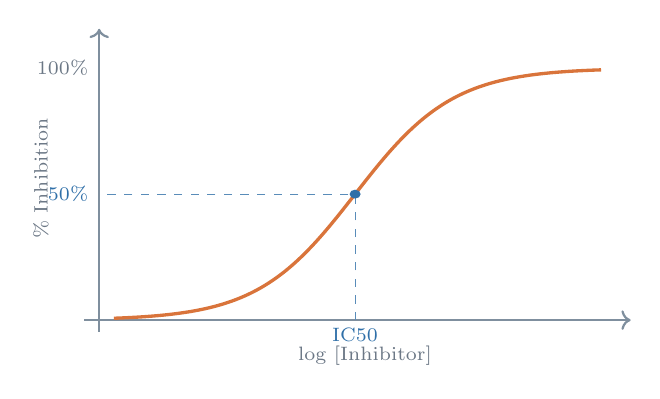
\begin{tikzpicture}[xscale=1.25,yscale=1.0]
        \draw[->,nxdark!55,thick] (-0.15,0) -- (5.4,0);
        \draw[->,nxdark!55,thick] (0,-0.15) -- (0,3.7);
        \node[lbl,below] at (2.7,-0.25) {\e{log [Inhibitor]}};
        \node[lbl,rotate=90,above] at (-0.45,1.8) {\e{\% Inhibition}};

        \draw[nxaccent,very thick] plot[domain=0.15:5.1,samples=90,smooth]
             (\x,{3.2/(1+exp(-2.0*(\x-2.6)))});

        \draw[dashed,nxblue!80] (2.6,0) -- (2.6,1.6) -- (0,1.6);
        \fill[nxblue] (2.6,1.6) circle (1.6pt);
        \node[lbl,text=nxblue,below] at (2.6,-0.02) {\e{IC50}};
        \node[lbl,text=nxblue,left]  at (-0.05,1.6) {\e{50\%}};
        \node[lbl,left] at (-0.05,3.2) {\e{100\%}};
      \end{tikzpicture}

      \vspace{2mm}
      {\footnotesize\color{nxgray}
       منحنی پاسخ به غلظت؛ \e{IC50} نقطه‌ی رسیدن به نیمه‌ی حداکثر مهار است.}
    \end{column}
  \end{columns}
  \note{این تمایز را حتماً بگو، چون از نظر علمی مهم است و نشان می‌دهد ادبیات را دقیق خوانده‌ای: \e{Kd} و \e{Ki} معیار اتصال‌اند، \e{IC50} معیار اثر عملکردی. ادبیات مقایسه‌ی ابزارهای \e{DTA} هم صراحتاً روی همین تأکید می‌کند.}
\end{frame}

%---------------------------------------------------------------- 8 --
\begin{frame}{جمع‌بندی معیارهای اتصال و مهار}
  \framesubtitle{کدام معیار چه چیزی را می‌سنجد؟}
  \vspace{3mm}
  \centering
  {\small
  \rowcolors{2}{nxlight}{white}
  \begin{tabular}{p{0.16\textwidth} p{0.34\textwidth} p{0.28\textwidth}}
    \rowcolor{nxdark}
    \thd{معیار} & \thd{مفهوم} & \thd{مقدار کمتر یعنی} \\
    \E{Kd}   & \e{Dissociation constant}        & \e{affinity} بیشتر \\
    \E{pKd}  & \e{−log\textsubscript{10}(K\textsubscript{d})} & \e{affinity} بیشتر \\
    \E{Ki}   & \e{Inhibition constant}          & \e{affinity} بیشتر \\
    \E{pKi}  & \e{−log\textsubscript{10}(K\textsubscript{i})} & \e{affinity} بیشتر \\
    \E{IC50} & غلظت لازم برای ۵۰٪ مهار          & \e{potency} بیشتر \\
  \end{tabular}}

  \vspace{5mm}
  \begin{exampleblock}{کاربرد در عمل}
    در بسیاری از \e{benchmark}های \e{DTA}، مقادیر \e{affinity} به شکل
    \key{لگاریتمی} مانند \e{pKd} یا \e{pKi} استفاده می‌شوند.
    برای نمونه \e{DCGAN-DTA} روی \e{BindingDB} مقادیر را به \e{pKd} تبدیل کرده
    و \e{PDBBind} نیز شامل مقادیر \e{log-transformed} از \e{Ki} و \e{Kd} است.
  \end{exampleblock}
  \note{این اسلاید پل به بخش بعد است. بگو: «پس برچسبی که مدل‌ها پیش‌بینی می‌کنند معمولاً یک عدد پیوسته در مقیاس لگاریتمی است؛ حالا ببینیم پژوهشگران برای پیش‌بینی این عدد چه مسیری را طی کرده‌اند.»}
\end{frame}

%======================================================================
\section{مسیر پژوهشی}
%======================================================================

%---------------------------------------------------------------- 9 --
\begin{frame}{درخت تکاملی روش‌های پیش‌بینی \e{DTA}}
  \framesubtitle{از ۲۰۱۵ تا ۲۰۲۶ --- بر پایه‌ی مرور \e{Wang et al.}, \e{Biotechnology Advances}, ۲۰۲۶}
  \vspace{1mm}
  \centering
  \begin{tikzpicture}[x=1mm,y=1mm,
      tn/.style={nxn,minimum height=6.6mm,inner xsep=3pt,inner ysep=1.5pt,
                 font=\tiny,align=center},
      bus/.style={draw=nxdark!65,thick},
      dn/.style={-{Stealth[length=1.8mm,width=1.4mm]},draw=nxdark!65,thick}]

    % ---- tier A: the historical spine --------------------------------
    \node[tn,ghost,minimum width=34mm] (a1) at (22,27)  {\fa{شباهت و \e{Kernel}}\\\e{KronRLS} --- ۲۰۱۵};
    \node[tn,ghost,minimum width=34mm] (a2) at (64,27)  {\fa{یادگیری ماشین ویژگی‌محور}\\\e{SimBoost} --- ۲۰۱۷};
    \node[tn,model,minimum width=34mm] (a3) at (106,27) {\fa{یادگیری عمیق}\\\e{DeepDTA} --- ۲۰۱۸};
    \draw[dn] (a1)--(a2); \draw[dn] (a2)--(a3);

    % ---- tier B: three representation families -----------------------
    \node[tn,minimum width=34mm] (b1) at (22,12)  {\fa{توالی و} \e{CNN}\\\e{DeepDTA} $\cdot$ \e{WideDTA}};
    \node[tn,minimum width=34mm] (b2) at (64,12)  {\fa{گراف و} \e{GNN}\\\e{GraphDTA} $\cdot$ \e{MGraphDTA}};
    \node[tn,minimum width=34mm] (b3) at (106,12) {\fa{توجه و} \e{Transformer}\\\e{AttentionDTA} $\cdot$ \e{ELECTRA-DTA}};
    \draw[bus] (a3.south) -- (106,20);
    \draw[bus] (22,20) -- (106,20);
    \draw[dn] (22,20) -- (b1.north);
    \draw[dn] (64,20) -- (b2.north);
    \draw[dn] (106,20) -- (b3.north);

    % ---- tier C: representation learning -----------------------------
    \node[tn,model,minimum width=66mm] (rep) at (64,0)
      {\fa{یادگیری نمایش} --- \e{Representation Learning}};
    \draw[bus] (b1.south) -- (22,5.5);
    \draw[bus] (b2.south) -- (64,5.5);
    \draw[bus] (b3.south) -- (106,5.5);
    \draw[bus] (22,5.5) -- (106,5.5);
    \draw[dn] (64,5.5) -- (rep.north);

    % ---- tier D: three sibling branches of representation learning ---
    \node[tn,minimum width=34mm] (d1) at (22,-13)  {\fa{ترکیب چندوجهی}\\\e{Fusion} $\cdot$ \e{Multimodal}};
    \node[tn,res,minimum width=34mm,draw=nxaccent,line width=0.7pt] (d2) at (64,-13)
      {\fa{یادگیری نمایش مولد}\\\e{Generative}};
    \node[tn,minimum width=34mm] (d3) at (106,-13) {\fa{پیش‌آموزش‌دیده}\\\e{Protein} \& \e{Chemical LM}};
    \draw[bus] (rep.south) -- (64,-7);
    \draw[bus] (22,-7) -- (106,-7);
    \draw[dn] (22,-7) -- (d1.north);
    \draw[dn] (64,-7) -- (d2.north);
    \draw[dn] (106,-7) -- (d3.north);

    % ---- tier E: the two papers this thesis studies -------------------
    \node[tn,minimum width=32mm,fill=nxblue!25,draw=nxblue,line width=0.7pt,
          font=\tiny\bfseries] (e1) at (44,-27) {\e{GAN} $\rightarrow$ \e{DCGAN-DTA} --- ۲۰۲۴};
    \node[tn,minimum width=32mm,fill=nxteal!25,draw=nxteal,line width=0.7pt,
          font=\tiny\bfseries] (e2) at (84,-27) {\e{VAE} $\rightarrow$ \e{Co-VAE} --- ۲۰۲۲};
    \draw[bus] (d2.south) -- (64,-20);
    \draw[bus] (44,-20) -- (84,-20);
    \draw[dn] (44,-20) -- (e1.north);
    \draw[dn] (84,-20) -- (e2.north);
  \end{tikzpicture}

  \vspace{1mm}
  {\scriptsize\color{nxgray}
   هر شاخه پاسخی به یک محدودیت متفاوت است --- \key{نه جانشین کامل نسل قبلی}.
   دو برگ پررنگ، نقطه‌ی ورود این پایان‌نامه‌اند.}
  \note{مهم‌ترین اسلاید بخش دوم؛ حدود دو تا سه دقیقه رویش وقت بگذار. دو پیام اصلی: (۱) این یک زنجیره‌ی خطی نیست، یک درخت است و شاخه‌های پایینی هم‌زمان‌اند نه پشت سر هم؛ (۲) \e{Generative} یک شاخه‌ی هم‌رده‌ی \e{Fusion} و \e{Pre-trained} است، نه مرحله‌ی بعد از \e{GNN}. در پایان انگشت بگذار روی دو برگ پررنگ و بگو «پایان‌نامه دقیقاً اینجاست».}
\end{frame}

%--------------------------------------------------------------- 10 --
\begin{frame}{مرحله‌ی اول: شباهت و \e{Kernel}}
  \framesubtitle{\e{KronRLS} --- \e{Pahikkala et al.}, ۲۰۱۵}
  \vspace{2mm}
  \begin{columns}[T]
    \begin{column}{0.50\textwidth}
      \small
      \begin{block}{فرض اصلی این نسل}
        اگر دو دارو از نظر شیمیایی شبیه باشند، احتمالاً \e{affinity} مشابهی
        دارند؛ پروتئین‌های مشابه نیز الگوی \e{binding} مشابهی دارند.
      \end{block}

      \vspace{1mm}
      \begin{exampleblock}{\e{KronRLS}}
        \small
        \e{Kronecker Regularized Least Squares} --- شباهت دارو--دارو و
        هدف--هدف را ترکیب می‌کند و مسئله را در قالب
        \e{regularized least squares} حل می‌کند.
      \end{exampleblock}
    \end{column}

    \begin{column}{0.46\textwidth}
      \centering
      \begin{tikzpicture}[x=1mm,y=1mm,font=\scriptsize]
        \node[drug,minimum width=25mm]  (s1) at (0,14)   {\fa{شباهت دارو}};
        \node[targ,minimum width=25mm]  (s2) at (30,14)  {\fa{شباهت پروتئین}};
        \node[model,minimum width=36mm] (k)  at (15,2)   {\e{Kernel} / \e{KronRLS}};
        \node[res,minimum width=25mm]   (a)  at (15,-11) {\e{Affinity}};
        \draw[arr] (s1)--(k); \draw[arr] (s2)--(k); \draw[arr] (k)--(a);
      \end{tikzpicture}

      \vspace{2mm}
      \begin{alertblock}{محدودیت}
        \small مدل فقط به اندازه‌ی کیفیت \e{similarity}ای که \key{انسان}
        تعریف کرده خوب بود؛ نمایش هنوز دستی و از پیش تعریف‌شده است.
      \end{alertblock}
    \end{column}
  \end{columns}
  \note{کوتاه رد شو. پیام: کیفیت مدل عملاً برابر بود با کیفیت تابع شباهتی که انسان تعریف می‌کرد. \e{KronRLS} هنوز هم یکی از \e{baseline}های استاندارد است و \e{DeepDTA} مستقیماً با آن مقایسه می‌شود.}
\end{frame}

%--------------------------------------------------------------- 11 --
\begin{frame}{مرحله‌ی دوم: یادگیری ماشین ویژگی‌محور}
  \framesubtitle{\e{SimBoost} --- \e{He et al.}, ۲۰۱۷}
  \vspace{2mm}
  \begin{columns}[T]
    \begin{column}{0.48\textwidth}
      \small
      \begin{block}{ویژگی‌های صریح به جای شباهت صرف}
        \begin{itemize}\itemsep0.2ex
          \item دارو: \e{fingerprints}، \e{descriptors}، ویژگی‌های ساختاری دوبعدی
          \item پروتئین: شباهت توالی، ویژگی‌های فیزیکوشیمیایی، اطلاعات تکاملی
          \item جفت دارو--هدف: ویژگی‌های شبکه‌ای
        \end{itemize}
      \end{block}

      \vspace{1mm}
      {\footnotesize
       \e{SimBoost} به جای \e{kernel} ساده از \E{Gradient Boosting Machines}
       استفاده کرد و توانست روابط \key{غیرخطی‌تر} را مدل کند.}
    \end{column}

    \begin{column}{0.48\textwidth}
      \centering
      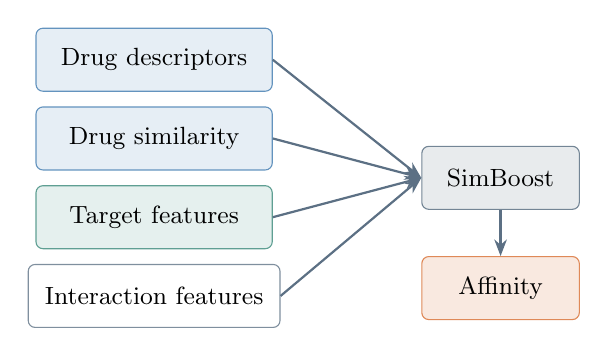
\begin{tikzpicture}[x=1mm,y=1mm,font=\scriptsize]
        \node[drug,minimum width=30mm]  (f1) at (0,16)  {\e{Drug descriptors}};
        \node[drug,minimum width=30mm]  (f2) at (0,6)   {\e{Drug similarity}};
        \node[targ,minimum width=30mm]  (f3) at (0,-4)  {\e{Target features}};
        \node[nxn,minimum width=30mm]   (f4) at (0,-14) {\e{Interaction features}};
        \node[model,minimum width=20mm] (sb) at (44,1)  {\e{SimBoost}};
        \node[res,minimum width=20mm]   (af) at (44,-13) {\e{Affinity}};
        \draw[arr] (f1.east) -- (sb.west);
        \draw[arr] (f2.east) -- (sb.west);
        \draw[arr] (f3.east) -- (sb.west);
        \draw[arr] (f4.east) -- (sb.west);
        \draw[arr] (sb) -- (af);
      \end{tikzpicture}

      \vspace{2mm}
      \begin{alertblock}{گلوگاه جابه‌جا شد}
        \small از \e{Similarity Engineering} به \key{\e{Feature Engineering}} ---
        ولی هنوز انسان در حلقه است.
      \end{alertblock}
    \end{column}
  \end{columns}
  \note{پیام کوتاه: پیشرفت واقعی بود (مدل‌سازی غیرخطی)، ولی گلوگاه فقط یک قدم عقب‌تر رفت. این همان چیزی است که یادگیری عمیق در مرحله‌ی بعد حذفش می‌کند.}
\end{frame}

%--------------------------------------------------------------- 12 --
\begin{frame}{مرحله‌ی سوم: ورود یادگیری عمیق}
  \framesubtitle{\e{DeepDTA} --- \e{Öztürk et al.}, ۲۰۱۸ \quad$\cdot$\quad \e{WideDTA}, ۲۰۱۹}
  \vspace{2mm}
  \centering
  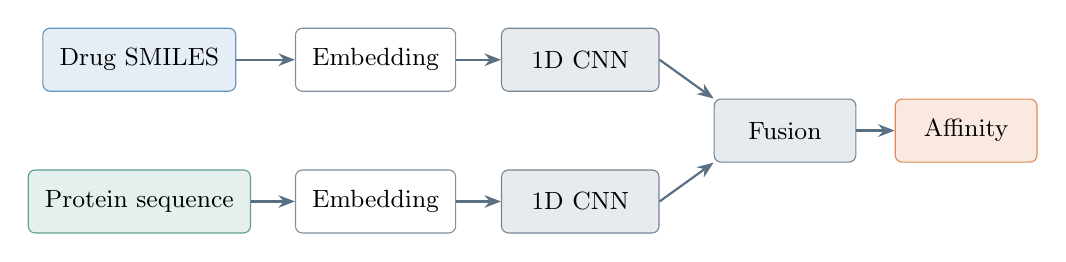
\begin{tikzpicture}[x=1mm,y=1mm,font=\scriptsize]
    \node[drug,minimum width=24mm]  (sm) at (12,10)  {\e{Drug SMILES}};
    \node[targ,minimum width=24mm]  (pr) at (12,-8)  {\e{Protein sequence}};
    \node[nxn,minimum width=20mm]   (e1) at (42,10)  {\e{Embedding}};
    \node[nxn,minimum width=20mm]   (e2) at (42,-8)  {\e{Embedding}};
    \node[model,minimum width=20mm] (c1) at (68,10)  {\e{1D CNN}};
    \node[model,minimum width=20mm] (c2) at (68,-8)  {\e{1D CNN}};
    \node[model,minimum width=18mm] (fu) at (94,1)   {\e{Fusion}};
    \node[res,minimum width=18mm]   (af) at (117,1)  {\e{Affinity}};
    \draw[arr] (sm)--(e1); \draw[arr] (e1)--(c1);
    \draw[arr] (pr)--(e2); \draw[arr] (e2)--(c2);
    \draw[arr] (c1.east) -- (fu.north west);
    \draw[arr] (c2.east) -- (fu.south west);
    \draw[arr] (fu)--(af);
  \end{tikzpicture}

  \vspace{3mm}
  \begin{columns}[T]
    \begin{column}{0.48\textwidth}
      \begin{alertblock}{تغییر بنیادی}
        \small
        نمایش دیگر به‌طور کامل توسط انسان تعریف نمی‌شود؛
        \key{شبکه آن را از داده‌ی خام یاد می‌گیرد}.
      \end{alertblock}
    \end{column}
    \begin{column}{0.48\textwidth}
      \begin{exampleblock}{\e{WideDTA} --- گام بعدی}
        \small
        افزودن \e{protein domains/motifs} و
        \e{maximum common substructure} برای نمایشی غنی‌تر.
      \end{exampleblock}
    \end{column}
  \end{columns}
  \note{\e{DeepDTA} نقطه‌ی عطف این حوزه است و تقریباً همه‌ی مقالات بعدی با آن مقایسه می‌شوند. اگر وقت کم بود، فقط همین اسلاید را از کل بخش بگو.}
\end{frame}

%--------------------------------------------------------------- 13 --
\begin{frame}{مرحله‌ی چهارم: گراف و نمایش ساختارآگاه}
  \framesubtitle{\e{GraphDTA} --- \e{Nguyen et al.}, ۲۰۲۱}
  \vspace{2mm}
  \begin{columns}[T]
    \begin{column}{0.50\textwidth}
      \centering
      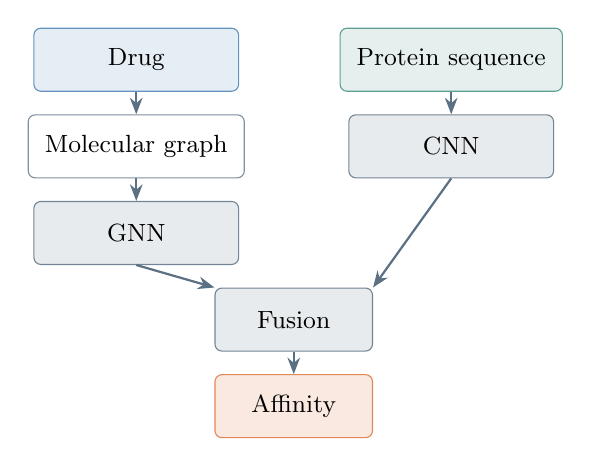
\begin{tikzpicture}[x=1mm,y=1mm,font=\scriptsize]
        \node[drug,minimum width=26mm]  (d)  at (0,18)  {\e{Drug}};
        \node[nxn,minimum width=26mm]   (g)  at (0,7)   {\e{Molecular graph}};
        \node[model,minimum width=26mm] (gn) at (0,-4)  {\e{GNN}};
        \node[targ,minimum width=26mm]  (p)  at (40,18) {\e{Protein sequence}};
        \node[model,minimum width=26mm] (cn) at (40,7)  {\e{CNN}};
        \node[model,minimum width=20mm] (fu) at (20,-15) {\e{Fusion}};
        \node[res,minimum width=20mm]   (af) at (20,-26) {\e{Affinity}};
        \draw[arr] (d)--(g); \draw[arr] (g)--(gn);
        \draw[arr] (p)--(cn);
        \draw[arr] (gn.south) -- (fu.north west);
        \draw[arr] (cn.south) -- (fu.north east);
        \draw[arr] (fu)--(af);
      \end{tikzpicture}
    \end{column}

    \begin{column}{0.46\textwidth}
      \small
      \begin{block}{چرا گراف؟}
        \e{SMILES} فقط یک \key{سریال‌سازی} از مولکول است، در حالی که مولکول
        ذاتاً یک گراف است: اتم $\rightarrow$ \e{Node}، پیوند $\rightarrow$ \e{Edge}.
      \end{block}

      \vspace{1mm}
      {\footnotesize
       \e{GraphDTA} چند معماری را بررسی کرد:
       \e{GCN} $\cdot$ \e{GAT} $\cdot$ \e{GAT-GCN} $\cdot$ \e{GIN}.}

      \vspace{2mm}
      \begin{exampleblock}{نتیجه}
        \small مسئله فقط عمیق‌تر کردن شبکه نبود؛ \key{نوع نمایش} هم تغییر کرد:
        از \e{sequence representation} به \e{structure-aware representation}.
      \end{exampleblock}
    \end{column}
  \end{columns}
  \note{اگر پرسیده شد چرا گراف بهتر است: چون اطلاعات ساختاری (حلقه‌ها، شاخه‌ها، همسایگی اتم‌ها) در \e{SMILES} به‌صورت ضمنی و در گراف به‌صورت صریح کد می‌شود. وارد جزئیات \e{GNN} نشو، موضوع پایان‌نامه نیست.}
\end{frame}

%--------------------------------------------------------------- 14 --
\begin{frame}{مرحله‌ی پنجم: توجه و \e{Transformer}}
  \framesubtitle{\e{AttentionDTA} $\cdot$ \e{ELECTRA-DTA} $\cdot$ \e{FusionDTA}, ۲۰۲۲}
  \vspace{2mm}
  \begin{columns}[T]
    \begin{column}{0.48\textwidth}
      \small
      \begin{block}{پرسش تازه}
        حتی با نمایش خوب، هنوز باید مشخص شود \key{کدام بخش} از دارو و
        کدام بخش از پروتئین برای \e{binding} مهم‌تر است.
      \end{block}

      \vspace{1mm}
      \begin{exampleblock}{\e{FusionDTA}}
        \small
        تمرکز بر \e{feature aggregation} با
        \e{attention-based feature polymerization} و
        \e{knowledge distillation}.
      \end{exampleblock}
    \end{column}

    \begin{column}{0.48\textwidth}
      \centering
      \vspace{1mm}
      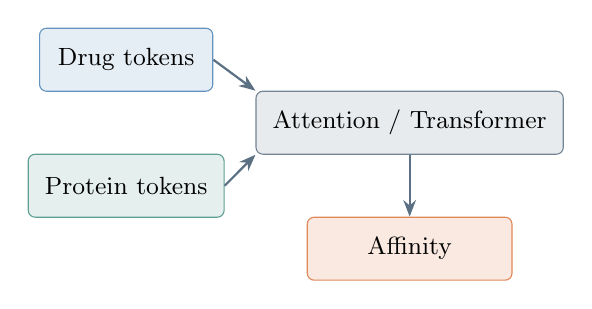
\begin{tikzpicture}[x=1mm,y=1mm,font=\scriptsize]
        \node[drug,minimum width=22mm]  (d) at (0,12)  {\e{Drug tokens}};
        \node[targ,minimum width=22mm]  (p) at (0,-4)  {\e{Protein tokens}};
        \node[model,minimum width=30mm] (at) at (36,4) {\e{Attention} / \e{Transformer}};
        \node[res,minimum width=26mm]   (af) at (36,-12) {\e{Affinity}};
        \draw[arr] (d.east) -- (at.north west);
        \draw[arr] (p.east) -- (at.south west);
        \draw[arr] (at)--(af);
      \end{tikzpicture}

      \vspace{2mm}
      {\footnotesize\color{nxgray}
       \e{CNN} برای الگوهای \e{local} مناسب است؛ \e{attention} می‌تواند
       وابستگی‌های دوربرد و میان‌وجهی را مدل کند.}
    \end{column}
  \end{columns}

  \vspace{1mm}
  \centering
  {\footnotesize
   تمرکز از «چه ویژگی‌ای استخراج کنیم؟» به
   \key{«چگونه ویژگی‌ها را با هم تعامل دهیم؟»} منتقل شد.}
  \note{این مرحله در نسخه‌ی قبلی ارائه غایب بود. نکته‌ی کلیدی: \e{attention} یک نوع نمایش جدید نمی‌سازد، بلکه نحوه‌ی ترکیب نمایش‌های موجود را یاد می‌گیرد.}
\end{frame}

%--------------------------------------------------------------- 15 --
\begin{frame}{مرحله‌ی ششم: چندوجهی و مدل‌های پیش‌آموزش‌دیده}
  \framesubtitle{\e{Multi-modal fusion} و \e{Protein/Chemical Language Models}}
  \vspace{2mm}
  \begin{columns}[T]
    \begin{column}{0.44\textwidth}
      \small
      \begin{block}{یک نمایش کافی نیست}
        \begin{itemize}\itemsep0.2ex
          \item دارو: \e{SMILES}، گراف مولکولی، \e{descriptors}
          \item پروتئین: توالی، ساختار، \e{binding site}، اطلاعات تکاملی
        \end{itemize}
      \end{block}

      \vspace{1mm}
      {\footnotesize
       نمونه‌ها: \e{DeepFusionDTA} $\cdot$ \e{MDF-DTA} $\cdot$
       \e{PocketDTA} $\cdot$ \e{GraphTransDTA}}
    \end{column}

    \begin{column}{0.52\textwidth}
      \centering
      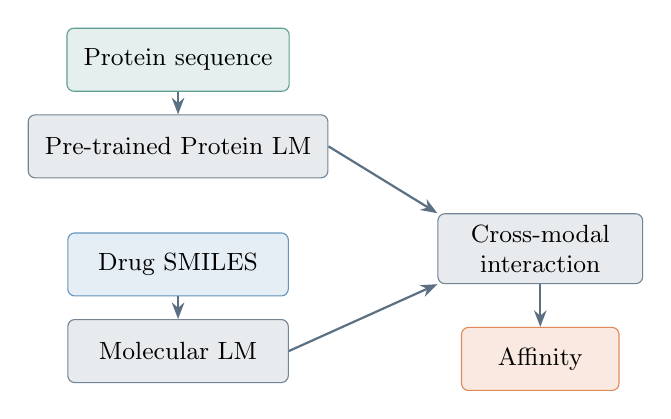
\begin{tikzpicture}[x=1mm,y=1mm,font=\scriptsize]
        \node[targ,minimum width=28mm]  (ps) at (0,14)  {\e{Protein sequence}};
        \node[model,minimum width=28mm] (pl) at (0,3)   {\e{Pre-trained Protein LM}};
        \node[drug,minimum width=28mm]  (ds) at (0,-12) {\e{Drug SMILES}};
        \node[model,minimum width=28mm] (ml) at (0,-23) {\e{Molecular LM}};
        \node[model,minimum width=26mm] (cx) at (46,-10) {\e{Cross-modal}\\\e{interaction}};
        \node[res,minimum width=20mm]   (af) at (46,-24) {\e{Affinity}};
        \draw[arr] (ps)--(pl); \draw[arr] (ds)--(ml);
        \draw[arr] (pl.east) -- (cx.north west);
        \draw[arr] (ml.east) -- (cx.south west);
        \draw[arr] (cx)--(af);
      \end{tikzpicture}

      \vspace{1mm}
      {\footnotesize\color{nxgray}
       \e{ESM} $\cdot$ \e{ProtBERT} $\cdot$ \e{ChemBERT} --- در مرور ۲۰۲۶،
       مدل‌های پیش‌آموزش‌دیده یک \key{پارادایم مستقل} شمرده می‌شوند.}
    \end{column}
  \end{columns}
  \note{این مرحله هم در نسخه‌ی قبلی غایب بود و اضافه‌کردنش نشان می‌دهد ادبیات را تا ۲۰۲۶ دنبال کرده‌ای. اگر استاد پرسید چرا از این مسیر استفاده نکرده‌ای، بگو موضوع پایان‌نامه شاخه‌ی مولد است و این شاخه‌ی موازی می‌تواند کار آینده باشد.}
\end{frame}

%--------------------------------------------------------------- 16 --
\begin{frame}{مرحله‌ی هفتم: یادگیری نمایش مولد}
  \framesubtitle{شاخه‌ای هم‌رده با \e{Fusion} و \e{Pre-trained} --- نه مرحله‌ی بعد از \e{GNN}}
  \vspace{2mm}
  \begin{columns}[T]
    \begin{column}{0.46\textwidth}
      \small
      \begin{block}{پرسش این شاخه}
        تا اینجا مدل‌ها یک نمایش می‌گیرند و \e{affinity} را پیش‌بینی می‌کنند.
        پرسش تازه: آیا می‌توان از \key{مدل‌های مولد} برای یادگیری
        \key{نمایش بهتر} استفاده کرد؟
      \end{block}

      \vspace{1mm}
      \begin{alertblock}{چرا این شاخه مهم است}
        \small
        \begin{itemize}\itemsep0.2ex
          \item بهره‌گیری از داده‌ی \key{بدون برچسب}
          \item فضای نهان ساختارمند و پیوسته
          \item امکان \e{pretraining} پیش از رگرسیون
        \end{itemize}
      \end{alertblock}
    \end{column}

    \begin{column}{0.50\textwidth}
      \centering
      \vspace{1mm}
      \begin{tikzpicture}[x=1mm,y=1mm,font=\scriptsize]
        \node[res,minimum width=40mm,draw=nxaccent,line width=0.7pt] (gm) at (30,16)
          {\fa{یادگیری نمایش مولد}};
        \node[nxn,minimum width=20mm,fill=nxblue!12,draw=nxblue!75] (gan) at (8,2)  {\E{GAN}};
        \node[nxn,minimum width=20mm,fill=nxteal!12,draw=nxteal!75] (vae) at (52,2) {\E{VAE}};
        \node[nxn,minimum width=26mm,fill=nxblue!25,draw=nxblue,font=\scriptsize\bfseries]
          (dc) at (8,-13) {\e{DCGAN-DTA}};
        \node[nxn,minimum width=26mm,fill=nxteal!25,draw=nxteal,font=\scriptsize\bfseries]
          (cv) at (52,-13) {\e{Co-VAE}};
        \draw[arr] (gm)--(gan); \draw[arr] (gm)--(vae);
        \draw[arr] (gan)--(dc); \draw[arr] (vae)--(cv);
        \node[lbl,text width=26mm,align=center] at (8,-23)  {\fa{یادگیری تخاصمی}};
        \node[lbl,text width=26mm,align=center] at (52,-23) {\fa{یادگیری وردشی}};
      \end{tikzpicture}
    \end{column}
  \end{columns}
  \note{اینجا پل اصلی ارائه است. جمله‌ی گذار: «این دو مقاله دو پاسخ متفاوت به یک پرسش واحدند؛ حالا هر کدام را جداگانه می‌بینیم.» حتماً تأکید کن که \e{Generative} از نظر تاریخی بعد از \e{GNN} نیامده، بلکه یک شاخه‌ی موازی است.}
\end{frame}

%--------------------------------------------------------------- 17 --
\begin{frame}{افق کنونی: ۲۰۲۶}
  \framesubtitle{\e{Foundation} $\cdot$ \e{Multimodal} $\cdot$ \e{Task-adaptive} $\cdot$ \e{Cold-start}}
  \vspace{3mm}
  \begin{columns}[T]
    \begin{column}{0.48\textwidth}
      \small
      \begin{block}{مسیرهای فعال امروز}
        \begin{itemize}\itemsep0.25ex
          \item نمایش‌های \e{pre-trained} در مقیاس بزرگ
          \item یادگیری \e{multimodal} (توالی + گراف + ساختار)
          \item \e{cross-modal interaction} به جای الحاق ساده
          \item تعمیم در شرایط \e{cold-start}
          \item \e{meta-learning} و \e{task adaptation}
          \item مدل‌های \e{binding-site-aware}
        \end{itemize}
      \end{block}
    \end{column}

    \begin{column}{0.48\textwidth}
      \vspace{1mm}
      \begin{exampleblock}{نمونه‌های ۲۰۲۶}
        \small
        \begin{itemize}\itemsep0.25ex
          \item \lr{A meta learning and task adaptive approach for DTA
                --- Nature Communications}
          \item \e{DCI-SiteDTA} --- ورود اطلاعات \e{binding site}
          \item \e{GraphTransDTA} --- \e{Graph Transformer} برای
                ترکیب داده‌های چندوجهی
        \end{itemize}
      \end{exampleblock}

      \vspace{1mm}
      {\footnotesize\color{nxgray}
       نکته‌ی مهم: \key{مسیر متوقف نشده}. شاخه‌ی مولد یکی از چند مسیر فعال است
       و این پایان‌نامه دقیقاً همان شاخه را بررسی می‌کند.}
    \end{column}
  \end{columns}
  \note{این اسلاید نشان می‌دهد که تصویر کاملی از حوزه داری و می‌دانی پایان‌نامه‌ات کجای آن می‌نشیند. اگر استاد پرسید «چرا سراغ \e{foundation models} نرفتی؟» بگو منابع محاسباتی و دامنه‌ی پایان‌نامه محدود است و این مسیر را به‌عنوان کار آینده مطرح می‌کنم.}
\end{frame}

%--------------------------------------------------------------- 18 --
\begin{frame}{جایگاه پایان‌نامه در این درخت}
  \framesubtitle{چرا دقیقاً این دو مقاله؟}
  \vspace{2mm}
  \centering
  \begin{tikzpicture}[x=1mm,y=1mm,font=\scriptsize,
      dn/.style={-{Stealth[length=1.9mm,width=1.5mm]},draw=nxdark!65,thick},
      bus/.style={draw=nxdark!65,thick}]
    \node[model,minimum width=28mm,minimum height=7mm] (dl)  at (64,18) {\fa{یادگیری عمیق}};
    \node[model,minimum width=44mm,minimum height=7mm] (rep) at (64,7)  {\e{Representation Learning}};
    \draw[dn] (dl)--(rep);

    \node[ghost,minimum width=17mm,minimum height=7mm] (s1) at (12,-7)  {\fa{توالی}};
    \node[ghost,minimum width=17mm,minimum height=7mm] (s2) at (33,-7)  {\fa{گراف}};
    \node[ghost,minimum width=17mm,minimum height=7mm] (s3) at (54,-7)  {\fa{توجه}};
    \node[ghost,minimum width=19mm,minimum height=7mm] (s4) at (77,-7)  {\fa{چندوجهی}};
    \node[res,minimum width=22mm,minimum height=7mm,draw=nxaccent,line width=0.7pt]
      (s5) at (105,-7) {\fa{مولد}};
    \draw[bus] (rep.south) -- (64,-1);
    \draw[bus] (12,-1) -- (105,-1);
    \foreach \n/\x in {s1/12,s2/33,s3/54,s4/77,s5/105} \draw[dn] (\x,-1) -- (\n.north);

    \node[nxn,minimum width=30mm,minimum height=7mm,fill=nxblue!25,draw=nxblue,
          line width=0.7pt,font=\scriptsize\bfseries] (dc) at (72,-22)
      {\e{GAN} $\rightarrow$ \e{DCGAN-DTA}};
    \node[nxn,minimum width=26mm,minimum height=7mm,fill=nxteal!25,draw=nxteal,
          line width=0.7pt,font=\scriptsize\bfseries] (cv) at (108,-22)
      {\e{VAE} $\rightarrow$ \e{Co-VAE}};
    \draw[bus] (s5.south) -- (105,-15);
    \draw[bus] (72,-15) -- (108,-15);
    \draw[dn] (72,-15) -- (dc.north);
    \draw[dn] (108,-15) -- (cv.north);
  \end{tikzpicture}

  \vspace{1mm}
  \begin{alertblock}{صورت‌بندی قابل دفاع}
    \centering
    \small
    این پژوهش ادعا نمی‌کند روش‌های پیشین ضعیف بوده‌اند؛ بلکه بر
    \key{شاخه‌ی یادگیری نمایش مولد} در تکامل روش‌های \e{DTA} تمرکز می‌کند و
    دو نماینده‌ی اصلی آن را زیر یک پروتکل مشترک مقایسه می‌کند.
  \end{alertblock}
  \note{این اسلاید پاسخ آماده به پرسش «چرا این دو مقاله؟» است. جمله‌ای که نباید بگویی: «روش‌های قبلی ضعیف بودند و من مدل بهتری می‌سازم» --- چون اثباتش نیازمند آزمایش گسترده است. جمله‌ای که باید بگویی: «این دو، نماینده‌های شاخص دو زیرشاخه‌ی یک پارادایم‌اند و تاکنون زیر یک پروتکل مشترک مقایسه نشده‌اند.»}
\end{frame}

%======================================================================
\section{مقاله‌ی اول: \e{DCGAN-DTA}}
%======================================================================

%--------------------------------------------------------------- 15 --
\begin{frame}{\e{DCGAN-DTA}}
  \framesubtitle{نماینده‌ی شاخه‌ی \e{GAN} \ --- \ \e{Kalemati et al.}, \e{BMC Genomics}, ۲۰۲۴}
  \vspace{2mm}
  \begin{columns}[T]
    \begin{column}{0.48\textwidth}
      \small
      \begin{alertblock}{چالش‌های مورد اشاره‌ی نویسندگان}
        \begin{itemize}\itemsep0.2ex
          \item داده‌ی آموزشی محدود (\e{limited training data})
          \item انتخاب و مهندسی ویژگی
          \item نیاز به اعتبارسنجی قوی‌تر
          \item \e{generalization} به داده‌های دیده‌نشده
        \end{itemize}
      \end{alertblock}

      \vspace{1mm}
      \centering
      \begin{tikzpicture}[node distance=5mm,font=\footnotesize]
        \node[model,minimum width=22mm] (g) {\e{Generator}};
        \node[model,minimum width=22mm,right=8mm of g] (d) {\e{Discriminator}};
        \draw[arr] (g) -- (d);
        \draw[arr,dashed] (d.south) .. controls +(0,-7mm) and +(0,-7mm) .. (g.south)
          node[lbl,midway,below] {\fa{سیگنال تخاصمی}};
      \end{tikzpicture}
    \end{column}

    \begin{column}{0.48\textwidth}
      \small
      \begin{block}{ایده}
        استفاده از \E{Deep Convolutional Generative Adversarial Network}
        برای \key{یادگیری نمایش} دارو و پروتئین.
      \end{block}

      \vspace{1mm}
      \begin{exampleblock}{چرا این مقاله مهم است}
        \footnotesize
        \e{DCGAN-DTA} را نباید «یک مدل \e{CNN} دیگر» دید. اهمیت آن در این است که
        ظرفیت \key{یادگیری نمایشِ} مدل‌های مولد را وارد مسئله‌ی \e{DTA} می‌کند و از
        \key{\e{pretraining}} --- از جمله روی داده‌ی بدون برچسب --- برای استخراج
        نمایش بهره می‌گیرد.
      \end{exampleblock}
    \end{column}
  \end{columns}
  \note{جمله‌ی کلیدی این اسلاید: «\e{DCGAN-DTA} تلاش می‌کند ظرفیت یادگیری نمایش مدل‌های مولد را وارد مسئله‌ی \e{DTA} کند و از \e{pretraining} برای استخراج نمایش استفاده کند.» حتماً تأکید کن که \e{GAN} اینجا برای تولید دارو به کار نمی‌رود، بلکه برای یادگیری نمایش --- این تفاوت ظریف ولی مهمی است و معمولاً همین‌جا سؤال می‌شود.}
\end{frame}

%--------------------------------------------------------------- 16 --
\begin{frame}{معماری \e{DCGAN-DTA}}
  \framesubtitle{نمودار بلوکی مقاله --- \e{Kalemati et al.}, \e{BMC Genomics}, ۲۰۲۴}
  \vspace{1mm}
  \begin{columns}[c]
    \begin{column}{0.40\textwidth}
      \centering
      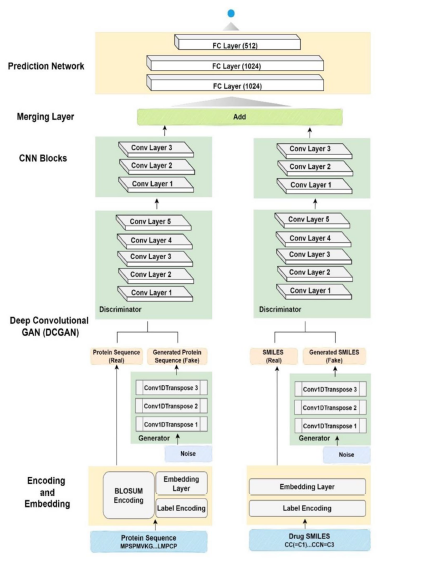
\includegraphics[width=0.96\linewidth]{presentation-figs/DCGAN-block-diagram.png}
    \end{column}

    \begin{column}{0.57\textwidth}
      \begin{block}{پنج مرحله --- شکل از پایین به بالا خوانده می‌شود}
        \footnotesize
        \begin{enumerate}\itemsep0.35ex
          \item کدگذاری و تعبیه --- \e{Label} / \e{BLOSUM} + \e{Embedding}
          \item پیش‌آموزش \e{DCGAN} --- \e{Generator} + \e{Discriminator}
          \item بلوک‌های \e{CNN} --- استخراج ویژگی
          \item لایه‌ی ادغام دو شاخه --- \e{Add}
          \item شبکه‌ی پیش‌بینی --- \e{FC 1024} $\rightarrow$ \e{512}
        \end{enumerate}
      \end{block}

      \vspace{1mm}
      \begin{alertblock}{نکته‌ی کلیدی}
        \footnotesize
        \e{GAN} اینجا \key{برای تولید دارو نیست}؛ \e{Generator} و
        \e{Discriminator} فقط برای \key{پیش‌آموزش نمایش} به کار می‌روند و
        نمایش آموخته‌شده به سر رگرسیون داده می‌شود.
      \end{alertblock}
    \end{column}
  \end{columns}
  \note{شکل را از پایین به بالا توضیح بده --- همان ترتیبی که در ستون کنارش شماره خورده است. دو شاخه‌ی چپ و راست شکل کاملاً متقارن‌اند؛ تنها تفاوت جدی، \e{BLOSUM encoding} در شاخه‌ی پروتئین است که اطلاعات تکاملی (شباهت جانشینی اسیدهای آمینه) را وارد مدل می‌کند. اگر وقت کم بود فقط بگو: کدگذاری، پیش‌آموزش تخاصمی، \e{CNN}، ادغام، رگرسیون.}
\end{frame}

%======================================================================
\section{مقاله‌ی دوم: \e{Co-VAE}}
%======================================================================

%--------------------------------------------------------------- 17 --
\begin{frame}{\e{Co-VAE}}
  \framesubtitle{نماینده‌ی شاخه‌ی \e{VAE} \ --- \ \e{Li, Zhao \& Li}, \e{IEEE TPAMI}, ۲۰۲۲}
  \vspace{3mm}
  \begin{columns}[T]
    \begin{column}{0.50\textwidth}
      \centering
      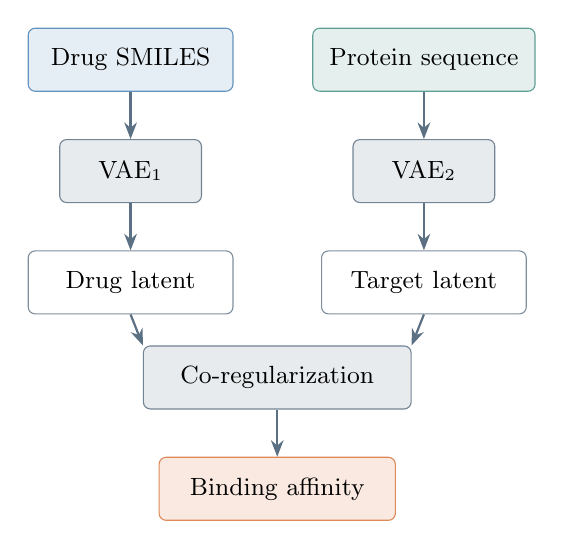
\begin{tikzpicture}[node distance=5mm,font=\footnotesize]
        \node[drug,minimum width=26mm] (d) {\e{Drug SMILES}};
        \node[model,minimum width=18mm,below=6mm of d] (v1) {\lr{$\text{VAE}_1$}};
        \node[nxn,minimum width=26mm,below=6mm of v1] (dl) {\e{Drug latent}};
        \draw[arr] (d)--(v1); \draw[arr] (v1)--(dl);

        \node[targ,minimum width=26mm,right=10mm of d] (t) {\e{Protein sequence}};
        \node[model,minimum width=18mm,below=6mm of t] (v2) {\lr{$\text{VAE}_2$}};
        \node[nxn,minimum width=26mm,below=6mm of v2] (tl) {\e{Target latent}};
        \draw[arr] (t)--(v2); \draw[arr] (v2)--(tl);

        \node[model,minimum width=34mm,below=8mm of $(dl)!0.5!(tl)$] (co) {\e{Co-regularization}};
        \node[res,minimum width=30mm,below=6mm of co] (af) {\e{Binding affinity}};
        \draw[arr] (dl.south) -- (co.north west);
        \draw[arr] (tl.south) -- (co.north east);
        \draw[arr] (co) -- (af);
      \end{tikzpicture}
    \end{column}

    \begin{column}{0.46\textwidth}
      \small
      \vspace{2mm}
      \begin{block}{ایده‌ی اصلی}
        دو \e{VAE} مجزا برای دارو و هدف، به‌همراه یک بخش
        \key{\e{co-regularization}} که فضاهای نهان را به مقدار
        \e{affinity} گره می‌زند.
      \end{block}

      \vspace{1.5mm}
      \begin{exampleblock}{چرا این مقاله مهم است}
        \footnotesize
        فضای نهان اینجا \key{احتمالاتی} است، نه یک بردار ثابت؛ و مدل فقط برای
        \e{prediction} طراحی نشده --- نویسندگان نشان می‌دهند می‌توان از آن برای
        \key{تولید داروهای جدید با هدف‌های مشابه} نیز استفاده کرد.
      \end{exampleblock}
    \end{column}
  \end{columns}
  \note{تفاوت بنیادی با مقاله‌ی قبل: آنجا نمایش با فرایند تخاصمی و در یک مرحله‌ی پیش‌آموزشِ جدا ساخته می‌شود؛ اینجا فضای نهان احتمالاتی است و بازسازی، هم‌تنظیمی و رگرسیون هم‌زمان آموزش می‌بینند. همین تقابل --- \e{Adversarial} در برابر \e{Variational} --- است که مقایسه‌ی این دو را برای پایان‌نامه ارزشمند می‌کند.}
\end{frame}

%--------------------------------------------------------------- 18 --
\begin{frame}{معماری \e{Co-VAE}}
  \framesubtitle{نمودار بلوکی مقاله --- \e{Li et al.}, \e{IEEE TPAMI}, ۲۰۲۲}
  \vspace{1mm}
  \begin{columns}[c]
    \begin{column}{0.36\textwidth}
      \centering
      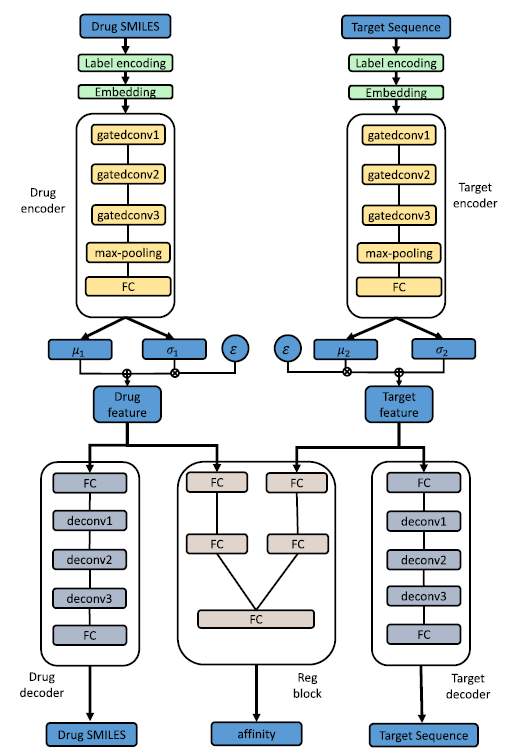
\includegraphics[width=0.94\linewidth]{presentation-figs/coVAE-block-diagram.png}
    \end{column}

    \begin{column}{0.61\textwidth}
      \begin{block}{مسیر بالا به پایین}
        \footnotesize
        \begin{enumerate}\itemsep0.3ex
          \item دو رمزگذار موازی --- \e{gatedconv}$\times$\e{3} + \e{max-pool} + \e{FC}
          \item فضای نهان --- \lr{$\mu$}، \lr{$\sigma$}، \lr{$\varepsilon$} و بازپارامتری‌سازی
        \end{enumerate}
      \end{block}

      \vspace{0.8mm}
      \begin{exampleblock}{سه سر خروجی از \e{drug} / \e{target feature}}
        \footnotesize
        \begin{itemize}\itemsep0.25ex
          \item \e{Drug decoder} --- بازسازی \e{SMILES}
          \item \E{Reg block} --- پیش‌بینی \key{\e{affinity}}
          \item \e{Target decoder} --- بازسازی توالی هدف
        \end{itemize}
      \end{exampleblock}

      \vspace{1.5mm}
      {\footnotesize\color{nxgray}
       همان دو فضای نهان هم‌زمان \key{بازسازی} و \key{رگرسیون} را تغذیه
       می‌کنند؛ همین اشتراک نقش \e{co-regularization} را بازی می‌کند.}
    \end{column}
  \end{columns}
  \note{تفاوت ساختاری مهم با \e{DCGAN-DTA}: آنجا پیش‌آموزش و رگرسیون دو مرحله‌ی جدا بودند، اینجا بازسازی و رگرسیون هم‌زمان و از یک فضای نهان مشترک آموزش می‌بینند. اگر پرسیده شد \e{co-regularization} دقیقاً چیست: یک جمله‌ی اضافه در تابع هزینه، علاوه بر دو جمله‌ی بازسازی و دو جمله‌ی \e{KL}، که فضاهای نهان دارو و هدف را طوری شکل می‌دهد که از رویشان بتوان \e{affinity} را بازیابی کرد.}
\end{frame}

%======================================================================
\section{مقایسه و خلأ پژوهشی}
%======================================================================

%--------------------------------------------------------------- 19 --
\begin{frame}{مقایسه‌ی دو رویکرد}
  \framesubtitle{\e{DCGAN-DTA} در برابر \e{Co-VAE}}
  \vspace{2mm}
  \centering
  {\footnotesize
  \rowcolors{2}{nxlight}{white}
  \begin{tabular}{p{0.22\textwidth} p{0.30\textwidth} p{0.30\textwidth}}
    \rowcolor{nxdark}
    \thd{ویژگی} & \thd{\e{DCGAN-DTA}} & \thd{\e{Co-VAE}} \\
    نوع مدل            & \e{GAN}                          & \e{VAE} \\
    ایده‌ی اصلی        & \e{Adversarial learning}         & \e{Variational learning} \\
    اجزا               & \e{Generator} + \e{Discriminator}& \e{Encoder} + \e{Decoder} \\
    فضای نهان          & تخاصمی / مولد                    & احتمالاتی \\
    نمایش دارو         & \e{SMILES}                       & \e{SMILES} \\
    نمایش هدف          & \e{Protein sequence}             & \e{Protein sequence} \\
    خروجی              & \e{Prediction}                   & \e{Prediction} + \e{co-regularization} \\
    هدف جانبی          & یادگیری نمایش                    & تولید + یادگیری نمایش \\
  \end{tabular}}

  \vspace{4mm}
  \begin{alertblock}{جمله‌ی کلیدی}
    \centering
    تفاوت اصلی این دو مقاله فقط در \e{architecture} نیست؛ آن‌ها
    \key{دو دیدگاه متفاوت} نسبت به یادگیری نمایش دارند.
  \end{alertblock}
  \note{این جدول را سطر به سطر نخوان. فقط سه سطر اول را بگو و مستقیم برو سراغ جمله‌ی پایین اسلاید، چون همان جمله ورودی بخش نوآوری است.}
\end{frame}

%--------------------------------------------------------------- 20 --
\begin{frame}{خلأ پژوهشی}
  \framesubtitle{\e{Research Gap}}
  \vspace{3mm}
  \begin{columns}[T]
    \begin{column}{0.47\textwidth}
      \begin{block}{\e{DCGAN-DTA}}
        \small تمرکز بر یادگیری نمایش مبتنی بر \e{GAN} برای \e{DTA}.
      \end{block}
      \vspace{2mm}
      \begin{exampleblock}{\e{Co-VAE}}
        \small تمرکز بر نمایش وردشی به‌همراه \e{co-regularization} برای \e{DTA}.
      \end{exampleblock}
    \end{column}

    \begin{column}{0.49\textwidth}
      \centering
      \vspace{1mm}
      \begin{tikzpicture}[font=\footnotesize,node distance=5mm]
        \node[nxn,minimum width=24mm,fill=nxblue!18,draw=nxblue!80] (a) {\e{DCGAN-DTA}};
        \node[nxn,minimum width=24mm,right=10mm of a,fill=nxteal!18,draw=nxteal!80] (b) {\e{Co-VAE}};
        \node[ghost,minimum width=40mm,below=10mm of $(a)!0.5!(b)$,draw=nxred!70,dashed,text=nxred]
          (g) {\fa{پروتکل آزمایشی مشترک؟}};
        \draw[arrd,draw=nxred!70] (a) -- (g);
        \draw[arrd,draw=nxred!70] (b) -- (g);
      \end{tikzpicture}
    \end{column}
  \end{columns}

  \vspace{4mm}
  \begin{alertblock}{خلأ}
    \centering
    مقایسه‌ی \key{مستقیم و کنترل‌شده}ی این دو پارادایم تحت یک
    \e{experimental protocol} مشترک، مسئله‌ای است که در این پایان‌نامه بررسی می‌شود.
  \end{alertblock}
  \note{اینجا محتاط باش و ادعای بزرگ نکن. نگو «هیچ‌کس این کار را نکرده»؛ بگو «تا جایی که بررسی کرده‌ام، مقایسه‌ی کنترل‌شده‌ی این دو خانواده تحت یک پروتکل یکسان کمتر انجام شده است». این جمله قابل دفاع‌تر است.}
\end{frame}

%======================================================================
\section{نوآوری پیشنهادی}
%======================================================================

%--------------------------------------------------------------- 21 --
\begin{frame}{نوآوری‌های پیشنهادی}
  \framesubtitle{چهار محور اصلی پایان‌نامه}
  \vspace{3mm}
  \begin{columns}[T]
    \begin{column}{0.48\textwidth}
      \small
      \begin{block}{۱. مقایسه‌ی دو پارادایم مولد}
        \e{Adversarial learning} در برابر \e{Variational learning}
        برای مسئله‌ی \e{DTA}.
      \end{block}

      \vspace{1mm}
      \begin{block}{۲. پروتکل آزمایشی یکسان}
        مجموعه‌داده، \e{preprocessing}، نمایش‌ها، \e{split}، معیارها و
        \e{seed}های کنترل‌شده --- تا تفاوت عملکرد واقعاً به
        \e{architecture} نسبت داده شود.
      \end{block}
    \end{column}

    \begin{column}{0.48\textwidth}
      \small
      \begin{block}{۳. بررسی \e{generalization}}
        مقایسه در دو شرایط \e{warm-start} و \e{cold-start}؛ عملکرد روی
        \e{random split} لزوماً توان پیش‌بینی برای داروها و هدف‌های
        واقعاً جدید را نشان نمی‌دهد.
      \end{block}

      \vspace{1mm}
      \begin{block}{۴. تحلیل فراتر از دقت}
        علاوه بر \e{performance}: \e{generalization}،
        \e{training stability}، \e{computational cost} و
        \e{data efficiency}.
      \end{block}
    \end{column}
  \end{columns}

  \vspace{3mm}
  \centering
  {\footnotesize\color{nxgray}
   \e{DCGAN-DTA} نیز همین مسئله را با \e{warm-start} و \e{cold-start} فیزیکوشیمیایی مورد توجه قرار داده است.}
  \note{مهم‌ترین اسلاید دفاع از نوآوری. اگر استاد گفت «این فقط مقایسه است، نوآوری نیست»، پاسخ آماده داشته باش: نوآوری در طراحی پروتکل کنترل‌شده و در تحلیل چندبعدی (نه صرفاً عدد دقت) است، و خروجی آن یک راهنمای انتخاب مدل برای این حوزه است.}
\end{frame}

%--------------------------------------------------------------- 22 --
\begin{frame}{سؤال اصلی پژوهش}
  \framesubtitle{پرسش اصلی و پرسش‌های فرعی}
  \vspace{2mm}
  \begin{alertblock}{پرسش اصلی}
    \centering
    آیا نوع روش یادگیری مولد --- \key{تخاصمی} یا \key{وردشی} --- می‌تواند بر
    کیفیت یادگیری نمایش و عملکرد پیش‌بینی قدرت اتصال در مسئله‌ی \e{DTA}
    تأثیر معناداری داشته باشد؟
  \end{alertblock}

  \vspace{1.5mm}
  \begin{block}{پرسش‌های فرعی}
    \footnotesize
    \begin{enumerate}\itemsep0.35ex
      \item کدام روش در \e{warm-start} عملکرد بهتری دارد؟
      \item کدام روش در \e{cold-start} بهتر \e{generalize} می‌کند؟
      \item حساسیت هر مدل نسبت به حجم داده چقدر است؟
      \item کدام مدل از نظر \e{computational cost} مناسب‌تر است؟
      \item آیا برتری مشاهده‌شده ناشی از \e{architecture} است یا از
            \e{dataset} / \e{split} / \e{preprocessing}؟
    \end{enumerate}
  \end{block}
  \note{ارائه باید با همین اسلاید به اوج برسد. پرسش پنجم مهم‌ترین است و نشان می‌دهد به اعتبار درونی آزمایش فکر کرده‌ای؛ روی همان یک مکث کوتاه کن.}
\end{frame}

%--------------------------------------------------------------- 23 --
\begin{frame}{روایت کلی ارائه}
  \framesubtitle{جمع‌بندی بصری مسیر ارائه}
  \vspace{3mm}
  \centering
  % سه سطر: صورت‌مسئله، مسیر روش‌ها، و جمع‌بندی به نوآوری
  \begin{tikzpicture}[x=1mm,y=1mm,font=\scriptsize]
    % --- row 1: the problem ---
    \node[ghost,minimum width=20mm] (dti) at (14,24) {\e{DTI}};
    \node[ghost,minimum width=20mm] (dta) at (44,24) {\e{DTA}};
    \node[nxn,minimum width=30mm]   (aff) at (84,24) {\e{Binding affinity}};
    \draw[arr] (dti)--(dta); \draw[arr] (dta)--(aff);
    % برچسب‌ها بالای سطر اول تا مسیر اتصال به سطر دوم آزاد بماند
    \node[lbl,text width=22mm,align=center] at (14,32) {\fa{هست یا نیست؟}};
    \node[lbl,text width=22mm,align=center] at (44,32) {\fa{چقدر قوی؟}};
    \node[lbl,text width=30mm,align=center] at (84,32) {\e{Kd} / \e{Ki} / \e{IC50}};

    % --- row 2: how the field got here ---
    \node[ghost,minimum width=18mm] (cls) at (11,4)  {\fa{کلاسیک}};
    \node[ghost,minimum width=13mm] (mlx) at (33,4)  {\e{ML}};
    \node[model,minimum width=13mm] (dlx) at (53,4)  {\e{DL}};
    \node[model,minimum width=32mm] (rep) at (87,4)  {\e{Representation learning}};
    \node[res,minimum width=18mm]   (gen) at (117,4) {\fa{مدل‌های مولد}};
    \draw[arr] (cls)--(mlx); \draw[arr] (mlx)--(dlx);
    \draw[arr] (dlx)--(rep); \draw[arr] (rep)--(gen);
    \draw[arr] (aff.south) -- ++(0,-6) -| (cls.north);

    % --- row 3: the two papers, the comparison, the contribution ---
    \node[nxn,minimum width=24mm,fill=nxblue!18,draw=nxblue!80] (g1) at (14,-16) {\e{DCGAN-DTA}};
    \node[nxn,minimum width=18mm,fill=nxteal!18,draw=nxteal!80] (g2) at (42,-16) {\e{Co-VAE}};
    \node[nxn,minimum width=30mm,draw=nxred!70,fill=nxred!8]    (cmp) at (80,-16) {\fa{مقایسه‌ی کنترل‌شده}};
    \node[res,minimum width=26mm,fill=nxaccent!30,draw=nxaccent] (nov) at (115,-16) {\fa{نوآوری پایان‌نامه}};
    \draw[arr] (g1)--(g2);
    \draw[arr] (g2)--(cmp);
    \draw[arr] (cmp)--(nov);
    \draw[arr] (gen.south) -- ++(0,-5) -| (g1.north);
  \end{tikzpicture}
  \note{این اسلاید جمع‌بندی بصری است. می‌توانی آن را ۱۵ ثانیه‌ای رد کنی یا اگر جلسه طولانی شد مستقیم از اسلاید ۲۲ به اسلاید پرسش‌ها بروی.}
\end{frame}

%--------------------------------------------------------------- 24 --
\begin{frame}{مراجع اصلی}
  \framesubtitle{منابع کلیدی این ارائه}
  \vspace{4mm}
  \small
  % هر مرجع یک بازه‌ی کامل چپ‌به‌راست است تا ترتیب اجزای استناد به‌هم نریزد
  \vspace{-2mm}
  \begin{enumerate}\footnotesize\itemsep0.35ex
    \item \lr{Wang et al., \textit{A unified survey on drug--target interaction
          and binding affinity prediction}, Biotechnology Advances, 2026.}
    \item \lr{Pahikkala et al., \textit{Toward more realistic drug--target
          interaction predictions} (KronRLS), Brief.\ Bioinform., 2015.}
    \item \lr{He et al., \textit{SimBoost: a read-across approach using gradient
          boosting machines}, J.\ Cheminformatics, 2017.}
    \item \lr{Öztürk et al., \textit{DeepDTA: deep drug--target binding affinity
          prediction}, Bioinformatics, 2018.}
    \item \lr{Öztürk et al., \textit{WideDTA: prediction of drug--target binding
          affinity}, arXiv, 2019.}
    \item \lr{Nguyen et al., \textit{GraphDTA: predicting drug--target binding
          affinity with graph neural networks}, Bioinformatics, 2021.}
    \item \lr{Li et al., \textit{Co-VAE: Drug--Target Binding Affinity Prediction
          by Co-Regularized Variational Autoencoders}, IEEE TPAMI, 2022.}
    \item \lr{Kalemati et al., \textit{DCGAN-DTA: Predicting drug--target binding
          affinity with deep convolutional GANs}, BMC Genomics, 2024.}
  \end{enumerate}

  \vspace{4mm}
  {\footnotesize\color{nxgray}
   فهرست کامل مراجع در متن پایان‌نامه ارائه شده است.}
  \note{این اسلاید فقط برای مستند بودن است؛ روی آن توقف نکن مگر استاد سؤال کند.}
\end{frame}

%--------------------------------------------------------------- 25 --
\begin{frame}[plain,noframenumbering]
  \vfill
  \begin{center}
    {\lr{\textcolor{nxaccent}{\rule{28mm}{1.6pt}}}}\\[6mm]
    {\Large\bfseries\color{nxdark} با تشکر از توجه شما}\\[5mm]
    {\large\color{nxgray} پرسش‌ها و پیشنهادها}\\[8mm]
    {\small محسن کاشفی کیا \quad$\cdot$\quad استاد راهنما: دکتر سایه میرزایی}
  \end{center}
  \vfill
  \note{آماده باش برای این سه سؤال: (۱) چرا همین دو مقاله را انتخاب کردی؟ (۲) داده و منابع محاسباتی را چطور تأمین می‌کنی؟ (۳) اگر نتیجه این شد که تفاوت معنادار نیست، دستاورد پایان‌نامه چیست؟ برای سؤال سوم پاسخ بده: نتیجه‌ی منفی هم یافته است، چون نشان می‌دهد تفاوت گزارش‌شده در مقالات ناشی از پروتکل بوده نه معماری.}
\end{frame}

\end{document}
"
%======================================================================
\documentclass[11pt,aspectratio=169,xcolor=table]{beamer}

\usetheme{default}
\usecolortheme{default}
\setbeamertemplate{navigation symbols}{}

\usepackage{amsmath,amssymb}
\usepackage{xcolor}
\usepackage{tikz}
\usetikzlibrary{arrows.meta,positioning,shapes.geometric,fit,backgrounds,calc,decorations.pathreplacing}
\usepackage{array}

%------------------------------- palette ------------------------------
\definecolor{nxdark}{HTML}{16334F}
\definecolor{nxblue}{HTML}{2F6FA8}
\definecolor{nxteal}{HTML}{2A7F6F}
\definecolor{nxaccent}{HTML}{D9743B}
\definecolor{nxred}{HTML}{B5453A}
\definecolor{nxgray}{HTML}{6B7785}
\definecolor{nxlight}{HTML}{EDF2F7}

%------------------------------- fonts --------------------------------
\usepackage{xepersian}
\settextfont[Scale=1.0]{XB Zar}
\setdigitfont[Scale=1.0]{XB Zar}
\setlatintextfont[Scale=0.92]{Cambria}

% سازگاری: وصله‌ی bidi برای jadval به ماکرویی ارجاع می‌دهد که از نسخه‌های
% جدید array.sty حذف شده است.
\providecommand\UseMathForPositioningText{}

%------------------------------ beamer look ---------------------------
\setbeamercolor{structure}{fg=nxdark}
\setbeamercolor{frametitle}{fg=white,bg=nxdark}
\setbeamercolor{framesubtitle}{fg=nxgray}
\setbeamercolor{footline}{fg=nxgray}
\setbeamercolor{normal text}{fg=nxdark!95}
\setbeamercolor{itemize item}{fg=nxaccent}
\setbeamercolor{itemize subitem}{fg=nxblue}
\setbeamercolor{block title}{fg=white,bg=nxblue}
\setbeamercolor{block body}{fg=nxdark,bg=nxblue!8}
\setbeamercolor{block title alerted}{fg=white,bg=nxaccent}
\setbeamercolor{block body alerted}{fg=nxdark,bg=nxaccent!10}
\setbeamercolor{block title example}{fg=white,bg=nxteal}
\setbeamercolor{block body example}{fg=nxdark,bg=nxteal!8}

\setbeamerfont{frametitle}{size=\large,series=\bfseries}
\setbeamerfont{framesubtitle}{size=\small}
\setbeamerfont{footline}{size=\scriptsize}
\setbeamerfont{block title}{size=\small,series=\bfseries}
\setbeamerfont{block body}{size=\small}

\setbeamertemplate{itemize item}{\raisebox{0.15ex}{\tiny$\blacktriangleleft$}}
\setbeamertemplate{itemize subitem}{\raisebox{0.15ex}{\tiny$\blacktriangleleft$}}
% قالب rounded بیمر با bidi به‌هم می‌ریزد؛ قالب ساده پایدار است.
\setbeamertemplate{blocks}[default]

% ---- frame title: full-width bar + accent rule ----
\definecolor{nxsub}{HTML}{A9BDD1}
\setbeamercolor{nxrule}{bg=nxaccent,fg=nxaccent}
\setbeamercolor{framesubtitle}{fg=nxsub,bg=nxdark}

% نکته‌ی مهم درباره‌ی bidi: در قالب‌های بیمر، فقط نخستین beamercolorbox رسم
% می‌شود و \rule داخل متن راست‌به‌چپ رنگ خود را از دست می‌دهد (سیاه می‌شود).
% بنابراین همه‌ی تزئینات (خط نارنجی سربرگ و نوار پیشرفت پاورقی) با tikz در
% قالب background canvas کشیده می‌شوند و سربرگ همیشه دو سطری است تا ارتفاع
% آن ثابت بماند.
\makeatletter
\setbeamertemplate{frametitle}{%
  \begin{beamercolorbox}[wd=\paperwidth,leftskip=1em,rightskip=1em]{frametitle}%
    \vspace{1.1ex}%
    {\usebeamerfont{frametitle}\insertframetitle}\\[0.1ex]%
    % هر اسلاید باید \framesubtitle داشته باشد تا ارتفاع سربرگ ثابت بماند و
    % خط نارنجیِ کشیده‌شده در background canvas دقیقاً زیر نوار بنشیند.
    {\usebeamerfont{framesubtitle}\usebeamercolor[fg]{framesubtitle}%
     \insertframesubtitle}%
    \vspace{1.0ex}%
  \end{beamercolorbox}%
}
\makeatother

% ---- footer: section name + frame number (chrome drawn in background) ----
\setbeamertemplate{footline}{%
  \begin{beamercolorbox}[wd=\paperwidth,ht=2.4ex,dp=1.4ex,leftskip=1em,rightskip=1em]{footline}%
    \usebeamerfont{footline}%
    \insertsectionhead\hfill\insertframenumber\,/\,\inserttotalframenumber%
  \end{beamercolorbox}%
}

% ---- all decorative chrome, drawn with tikz so bidi cannot swallow it ----
\newlength{\nxprogw}
\newlength{\nxhdrh}
\setlength{\nxhdrh}{37.2pt}    % ارتفاع نوار سربرگ (دو سطری، ثابت)
\makeatletter
\setbeamertemplate{background canvas}{%
  \setlength{\nxprogw}{\dimexpr\paperwidth/\inserttotalframenumber*\insertframenumber\relax}%
  \begin{tikzpicture}[overlay,remember picture]
    \fill[white] (current page.south west) rectangle (current page.north east);
    \ifbeamer@plainframe\else
      \fill[nxaccent] (current page.north west) ++(0,-\nxhdrh)
                      rectangle ++(\paperwidth,-1.2pt);
    \fi
    \fill[nxdark!12] (current page.south west) rectangle ++(\paperwidth,1pt);
    \fill[nxaccent]  (current page.south east) ++(-\nxprogw,0)
                     rectangle ++(\nxprogw,1pt);
  \end{tikzpicture}%
}
\makeatother

% ---- notes ----
\ifdefined\notesmode
  \setbeameroption{show only notes}
\else
  \setbeameroption{hide notes}
\fi
\setbeamerfont{note page}{size=\small}

%------------------------------ tikz styles ---------------------------
\tikzset{
  nxn/.style   ={draw=nxdark!55, rounded corners=2.5pt, fill=white,
                 inner xsep=6pt, inner ysep=4pt, minimum height=8mm,
                 font=\small, align=center},
  drug/.style  ={nxn, fill=nxblue!12,   draw=nxblue!75},
  targ/.style  ={nxn, fill=nxteal!12,   draw=nxteal!75},
  model/.style ={nxn, fill=nxdark!10,   draw=nxdark!60},
  res/.style   ={nxn, fill=nxaccent!16, draw=nxaccent!85},
  ghost/.style ={nxn, fill=nxlight,     draw=nxdark!25, text=nxgray},
  lbl/.style   ={font=\scriptsize, text=nxgray, inner sep=2pt},
  arr/.style   ={-{Stealth[length=2.1mm,width=1.6mm]}, draw=nxdark!70, thick},
  arrd/.style  ={arr, dashed},
  flat/.style  ={draw=none, fill=none, font=\small, align=center},
}

%-------------------------- small helper macros -----------------------
\newcommand{\E}[1]{\lr{\textbf{#1}}}
\newcommand{\e}[1]{\lr{#1}}
% متن فارسی داخل گره‌های tikz به صورت پاراگراف چپ‌به‌راست چیده می‌شود و ترتیب
% واژه‌ها برعکس می‌شود؛ \fa کل متن گره را در یک بازه‌ی راست‌به‌چپ قرار می‌دهد.
% توجه: داخل \fa نباید \\ بیاید — هر سطر را جداگانه باید پیچید.
\newcommand{\fa}[1]{\RLE{#1}}
% ریاضیِ نمایشی: \[...\] در ستون راست‌به‌چپ سرریز می‌کند و دیده نمی‌شود؛
% همچنین \lr باعث می‌شود ارقام داخل فرمول لاتین بمانند نه فارسی.
\newcommand{\disp}[1]{\begin{center}\lr{$\displaystyle #1$}\end{center}}
\newcommand{\key}[1]{\textcolor{nxaccent}{\textbf{#1}}}
\newcommand{\thd}[1]{\textcolor{white}{\textbf{#1}}}

% section divider
\AtBeginSection[]{%
  \begin{frame}[plain,noframenumbering]
    \vfill
    \begin{center}
      {\lr{\textcolor{nxaccent}{\rule{22mm}{1.6pt}}}}\\[4mm]
      {\usebeamerfont{frametitle}\Large\color{nxdark}\insertsectionhead}\\[3mm]
      {\lr{\textcolor{nxdark!20}{\rule{60mm}{0.7pt}}}}
    \end{center}
    \vfill
  \end{frame}
}

\begin{document}

%======================================================================
% TITLE
%======================================================================
\begin{frame}[plain,noframenumbering]
  \vspace{-3mm}
  \hbox to\textwidth{%
    
\includegraphics[height=11mm]{First-Pages/TehUni.png}\hfill
    
\includegraphics[height=11mm]{First-Pages/Eng.png}}

  \vspace{-6mm}
  \begin{center}
    {\footnotesize دانشگاه تهران — پردیس دانشکده‌های فنی}\\[0.4mm]
    {\footnotesize دانشکده علوم مهندسی — گروه الگوریتم‌ها و محاسبات}

    \vspace{3mm}
    {\lr{\textcolor{nxaccent}{\rule{30mm}{1.2pt}}}}

    \vspace{2.5mm}
    {\large\bfseries\color{nxdark} پیش‌بینی قدرت اتصال دارو--هدف\\[1mm]
     با مدل‌های مولد}\\[2mm]
    {\small\color{nxgray} مقایسه‌ی کنترل‌شده‌ی یادگیری تخاصمی و یادگیری وردشی}\\[0.6mm]
    {\scriptsize\color{nxgray}\e{Adversarial vs.\ Variational Representation Learning for Drug--Target Affinity}}

    \vspace{3mm}
    {\lr{\textcolor{nxdark!20}{\rule{70mm}{0.5pt}}}}\\[2mm]

    {\footnotesize ارائه‌دهنده: \textbf{محسن کاشفی کیا}}\\[0.8mm]
    {\footnotesize استاد راهنما: \textbf{دکتر سایه میرزایی}}\\[2mm]
    {\scriptsize\color{nxgray} گزارش پیشرفت پایان‌نامه کارشناسی ارشد \quad$\cdot$\quad شهریور ۱۴۰۵}
  \end{center}
  \note{سلام و تشکر از استاد. در یک جمله بگو: «هدف این جلسه این است که مسیر رسیدن از صورت‌مسئله تا نوآوری پیشنهادی پایان‌نامه را مرور کنیم.» زمان پیشنهادی کل ارائه: ۲۰ تا ۲۵ دقیقه.}
\end{frame}

%======================================================================
% OUTLINE
%======================================================================
\begin{frame}{فهرست مطالب}
  \framesubtitle{مسیر ارائه در یک نگاه}
  \vspace{3mm}
  \begin{columns}[T]
    \begin{column}{0.52\textwidth}
      \small
      \begin{enumerate}
        \item تعریف مسئله: از \e{DTI} تا \e{DTA}
        \item معیارهای کمی قدرت اتصال
        \item درخت تکاملی روش‌ها: از \e{KronRLS} تا مدل‌های بنیادی
        \item جایگاه پایان‌نامه در این درخت
        \item مقاله‌ی اول: \e{DCGAN-DTA} --- شاخه‌ی \e{GAN}
        \item مقاله‌ی دوم: \e{Co-VAE} --- شاخه‌ی \e{VAE}
        \item خلأ پژوهشی و نوآوری پیشنهادی
      \end{enumerate}
    \end{column}
    \begin{column}{0.44\textwidth}
      \begin{tikzpicture}[node distance=4.5mm,every node/.style={font=\scriptsize}]
        \node[ghost,minimum width=32mm] (a) {\fa{\e{DTI} — آیا برهم‌کنش هست؟}};
        \node[ghost,minimum width=32mm,below=of a] (b) {\fa{\e{DTA} — چقدر قوی است؟}};
        \node[model,minimum width=32mm,below=of b] (c) {\fa{مسیر پژوهشی تا مدل‌های مولد}};
        \node[res,minimum width=32mm,below=of c] (d) {\fa{نوآوری پیشنهادی}};
        \draw[arr] (a)--(b); \draw[arr] (b)--(c); \draw[arr] (c)--(d);
      \end{tikzpicture}
    \end{column}
  \end{columns}
  \note{این اسلاید نقشه‌ی راه است. یک جمله بگو: «ارائه از صورت‌مسئله شروع می‌شود، به دو مقاله‌ی مرجع می‌رسد و با سؤال پژوهشی پایان‌نامه تمام می‌شود.» روی آن معطل نشو.}
\end{frame}

%======================================================================
\section{تعریف مسئله}
%======================================================================

%---------------------------------------------------------------- 1 --
\begin{frame}{برهم‌کنش دارو--هدف چیست؟}
  \framesubtitle{\e{Drug--Target Interaction (DTI)}}
  \vspace{2mm}
  \begin{columns}[T]
    \begin{column}{0.46\textwidth}
      \small
      در فرآیند \e{drug discovery}، یکی از مسائل پایه شناسایی ارتباط میان
      \key{دارو} و \key{پروتئین هدف} است.

      \vspace{2mm}
      \begin{block}{پرسش \e{DTI}}
        آیا یک دارو می‌تواند با یک پروتئین هدف برهم‌کنش داشته باشد یا خیر؟
      \end{block}

      \vspace{1mm}
      {\footnotesize\color{nxgray}
       خروجی مسئله \key{دودویی} است: بله / خیر.}
    \end{column}
    \begin{column}{0.50\textwidth}
      \centering
      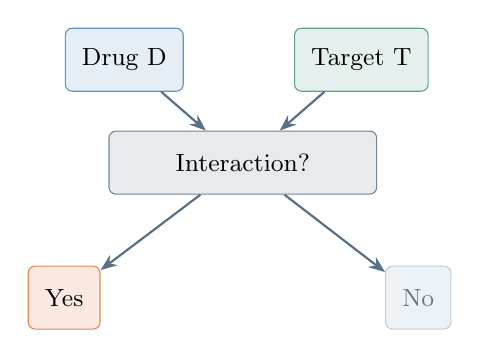
\begin{tikzpicture}[node distance=7mm]
        \node[drug]                       (d) {\e{Drug D}};
        \node[targ, right=14mm of d]      (t) {\e{Target T}};
        \node[model, below=9mm of $(d)!0.5!(t)$, minimum width=34mm] (i) {\e{Interaction?}};
        \node[res,  below left=9mm and 1mm of i]  (y) {\e{Yes}};
        \node[ghost,below right=9mm and 1mm of i] (n) {\e{No}};
        \draw[arr] (d) -- (i);
        \draw[arr] (t) -- (i);
        \draw[arr] (i) -- (y);
        \draw[arr] (i) -- (n);
      \end{tikzpicture}
    \end{column}
  \end{columns}
  \note{\e{DTI} را به عنوان مسئله‌ی پایه معرفی کن: «اگر بخواهیم فضای جستجوی \e{drug discovery} را کوچک کنیم، اولین سؤال این است که از میان تعداد زیادی دارو و پروتئین، کدام جفت‌ها احتمالاً با هم برهم‌کنش دارند.» مقاله‌ی \e{Co-VAE} هم مقدمه‌اش را از همین نقطه شروع می‌کند.}
\end{frame}

%---------------------------------------------------------------- 2 --
\begin{frame}{از تشخیص برهم‌کنش به اندازه‌گیری قدرت آن}
  \framesubtitle{چرا پاسخ بله/خیر کافی نیست؟}
  \vspace{1mm}
  \centering
  \begin{tikzpicture}[x=1mm,y=1mm,font=\footnotesize]
    % --- inputs ---
    \node[drug] (d1) at (0,7)   {\e{Drug A}};
    \node[drug] (d2) at (0,-7)  {\e{Drug B}};
    \node[targ] (tx) at (28,0)  {\e{Target X}};
    \draw[arr] (d1) -- (tx);
    \draw[arr] (d2) -- (tx);

    % --- DTI column ---
    \node[lbl,text=nxdark,font=\scriptsize\bfseries] at (60,17) {\fa{دیدِ \e{DTI}}};
    \node[res,minimum width=26mm]   (y1) at (60,7)  {\e{Yes}};
    \node[res,minimum width=26mm]   (y2) at (60,-7) {\e{Yes}};
    \draw[arr] (tx) -- (y1);
    \draw[arr] (tx) -- (y2);
    \node[lbl,text width=32mm,align=center] at (60,-17) {\fa{هر دو یکسان دیده می‌شوند}};

    % --- divider ---
    \draw[nxdark!20,thick] (80,20) -- (80,-20);

    % --- DTA column ---
    \node[lbl,text=nxdark,font=\scriptsize\bfseries] at (104,17) {\fa{دیدِ \e{DTA}}};
    \node[nxn,minimum width=28mm,fill=nxred!18,draw=nxred!80] (s1) at (104,7)  {\e{Strong binding}};
    \node[ghost,minimum width=28mm]                           (s2) at (104,-7) {\e{Weak binding}};
    \draw[arr,draw=nxdark!35] (y1) -- (s1);
    \draw[arr,draw=nxdark!35] (y2) -- (s2);
    \node[lbl,text width=34mm,align=center] at (104,-17) {\fa{دو دارو از هم تفکیک می‌شوند}};
  \end{tikzpicture}

  \vspace{2mm}
  \begin{alertblock}{پرسش دقیق‌تر}
    \centering قدرت اتصال دارو به هدف \key{چقدر} است؟ \quad$\Rightarrow$\quad مسئله‌ی \E{Drug--Target Binding Affinity (DTA)}
  \end{alertblock}
  \note{نکته‌ی کلیدی: دو دارو می‌توانند هر دو با یک \e{target} برهم‌کنش داشته باشند، ولی یکی اتصال بسیار قوی و دیگری اتصال ضعیف. \e{DTI} این تفاوت را نمی‌بیند. اینجا گذار از مسئله‌ی دسته‌بندی به مسئله‌ی رگرسیون اتفاق می‌افتد.}
\end{frame}

%---------------------------------------------------------------- 3 --
\begin{frame}{چرا \e{DTA}؟}
  \framesubtitle{اطلاعات کمی در برابر اطلاعات دودویی}
  \vspace{2mm}
  \centering
  {\small
  \rowcolors{2}{nxlight}{white}
  \begin{tabular}{p{0.34\textwidth} p{0.34\textwidth}}
    \rowcolor{nxdark}
    \thd{\e{DTI}} & \thd{\e{DTA}} \\
    آیا برهم‌کنش وجود دارد؟ & برهم‌کنش چقدر قوی است؟ \\
    خروجی دودویی (\e{binary})   & خروجی پیوسته (\e{continuous}) \\
    بله / خیر                & مقدار عددی \e{affinity} \\
    مناسب غربالگری اولیه     & مناسب رتبه‌بندی و اولویت‌دهی \\
  \end{tabular}}

  \vspace{4mm}
  \begin{columns}[c]
    \begin{column}{0.55\textwidth}
      \begin{exampleblock}{جمله‌ی کلیدی}
        \e{DTA} علاوه بر \key{وجود} برهم‌کنش، \key{شدت} آن را نیز مشخص می‌کند و
        بنابراین اطلاعات غنی‌تری در اختیار می‌گذارد.
      \end{exampleblock}
    \end{column}
    \begin{column}{0.42\textwidth}
      {\footnotesize\color{nxgray}
       \textbf{دقت در بیان:} نگوییم «\e{DTA} همیشه بهتر از \e{DTI} است»؛
       این‌ها دو صورت‌بندی متفاوت از مسئله‌اند. بگوییم برای \emph{هدف این پژوهش}،
       اطلاعات کمی \e{affinity} ارزشمندتر است.}
    \end{column}
  \end{columns}
  \note{حتماً تأکید کن که \e{DTA} و \e{DTI} دو \e{formulation} متفاوت‌اند، نه اینکه یکی مطلقاً بهتر از دیگری باشد. این جمله از نظر علمی قابل دفاع‌تر است و معمولاً همین‌جا سؤال پرسیده می‌شود. \e{Co-VAE} هم پیش‌بینی \e{affinity} را چالش‌برانگیزتر از تشخیص \e{interaction} می‌داند.}
\end{frame}

%---------------------------------------------------------------- 4 --
\begin{frame}{قدرت اتصال چگونه اندازه‌گیری می‌شود؟}
  \framesubtitle{نقشه‌ی معیارهای متداول}
  \vspace{4mm}
  \centering
  \begin{tikzpicture}[node distance=5mm]
    \node[model,minimum width=30mm] (root) {\fa{اندازه‌گیری \e{Affinity}}};

    \node[targ,minimum width=44mm,below right=12mm and 2mm of root] (ba) {\e{Binding affinity}\\[-1mm] \fa{{\scriptsize قدرت اتصال ترمودینامیکی}}};
    \node[res, minimum width=40mm,below left=12mm and 2mm of root]  (po) {\e{Potency / inhibition}\\[-1mm] \fa{{\scriptsize اثر عملکردی در آزمایش}}};

    \node[nxn,below left=10mm and -2mm of ba]  (kd) {\e{Kd} \ / \ \e{pKd}};
    \node[nxn,below right=10mm and -2mm of ba] (ki) {\e{Ki} \ / \ \e{pKi}};
    \node[nxn,below=10mm of po]                (ic) {\e{IC50}};

    \draw[arr] (root) -- (ba);
    \draw[arr] (root) -- (po);
    \draw[arr] (ba) -- (kd);
    \draw[arr] (ba) -- (ki);
    \draw[arr] (po) -- (ic);
  \end{tikzpicture}

  \vspace{3mm}
  {\footnotesize\color{nxgray}
   در اسلایدهای بعد هر معیار جداگانه تعریف می‌شود؛ تمایز ستون راست و چپ نکته‌ی اصلی این بخش است.}
  \note{این اسلاید «نقشه» است. فقط بگو چهار پنج اصطلاح داریم و مهم‌ترین نکته این است که \e{Kd} و \e{Ki} معیار \e{binding affinity} هستند ولی \e{IC50} معیار \e{potency} عملکردی است. جزئیات را در اسلایدهای بعد باز می‌کنی.}
\end{frame}

%---------------------------------------------------------------- 5 --
\begin{frame}{\e{Kd} و \e{pKd}}
  \framesubtitle{\e{Equilibrium Dissociation Constant}}
  \vspace{1mm}
  \begin{columns}[T]
    \begin{column}{0.50\textwidth}
      \small
      \begin{block}{تعریف مفهومی}
        \e{Kd} غلظتی از \e{ligand} است که در شرایط تعادل، تقریباً \key{نیمی} از
        \e{target}ها را در حالت \e{bound} قرار می‌دهد.
      \end{block}

      \vspace{-1mm}
      \disp{K_d \;=\; \frac{[D]\,[T]}{[DT]}}

      \vspace{-3mm}
      {\footnotesize
      \e{D}: داروی آزاد \quad $\cdot$ \quad \e{T}: هدف آزاد \quad $\cdot$ \quad \e{DT}: کمپلکس دارو--هدف}

      \vspace{2mm}
      \begin{alertblock}{مقیاس لگاریتمی}
        \vspace{-3mm}
        \disp{pK_d \;=\; -\log_{10}\!\big(K_d\,[M]\big)}
        \vspace{-3mm}
        \centering اگر \lr{$K_d = 10^{-9}\,M$} آنگاه \lr{$pK_d = 9$}
      \end{alertblock}
    \end{column}

    \begin{column}{0.46\textwidth}
      \centering
      \vspace{3mm}
      % مقیاس به‌صورت راست‌به‌چپ خوانده می‌شود: سمت راست = اتصال قوی
      \begin{tikzpicture}
        \shade[left color=nxlight,right color=nxred!55] (0,0) rectangle (6.4,0.55);
        \draw[nxdark!35] (0,0) rectangle (6.4,0.55);
        \node[lbl,below] at (5.8,0) {\fa{\e{Kd} کوچک}};
        \node[lbl,below] at (0.6,0) {\fa{\e{Kd} بزرگ}};
        \node[lbl,above,text=nxdark,font=\scriptsize\bfseries] at (5.4,0.55) {\fa{اتصال قوی}};
        \node[lbl,above,text=nxdark,font=\scriptsize\bfseries] at (1.0,0.55) {\fa{اتصال ضعیف}};

        \node[drug,minimum width=24mm,below=11mm of {(5.4,0)},font=\scriptsize] (a)
          {\e{Drug A}\\[-1mm]{\scriptsize\e{Kd = 1 nM}}};
        \node[ghost,minimum width=24mm,below=11mm of {(1.0,0)},font=\scriptsize] (b)
          {\e{Drug B}\\[-1mm]{\scriptsize\e{Kd = 100 nM}}};
      \end{tikzpicture}

      \vspace{6mm}
      {\small\color{nxdark}
       \lr{$K_d \downarrow$} \quad$\Longrightarrow$\quad \e{affinity} \lr{$\uparrow$} \quad$\Longrightarrow$\quad \lr{$pK_d \uparrow$}}
    \end{column}
  \end{columns}
  \note{نکته‌ای که معمولاً پرسیده می‌شود: چرا لگاریتم می‌گیریم؟ چون مقادیر \e{Kd} در بازه‌ای بسیار وسیع و بسیار کوچک (نانومولار تا میکرومولار) پخش‌اند و مقیاس لگاریتمی هم عددها را قابل‌مدیریت می‌کند و هم برای رگرسیون مناسب‌تر است. جهت را اشتباه نگو: \e{Kd} کمتر یعنی \e{affinity} بیشتر.}
\end{frame}

%---------------------------------------------------------------- 6 --
\begin{frame}{\e{Ki} و \e{pKi}}
  \framesubtitle{\e{Inhibition Constant}}
  \vspace{2mm}
  \begin{columns}[T]
    \begin{column}{0.50\textwidth}
      \small
      \begin{block}{تعریف}
        \e{Ki} معیاری برای بیان \e{affinity} یک \key{مهارکننده} (\e{inhibitor})
        نسبت به \e{target} یا آنزیم است.
      \end{block}

      \vspace{1mm}
      هرچه \e{Ki} کوچک‌تر باشد، \e{inhibitor} تمایل بیشتری به اتصال مؤثر
      به \e{target} دارد.

      \vspace{-1mm}
      \disp{pK_i \;=\; -\log_{10}\!\big(K_i\,[M]\big)}

      \vspace{-2mm}
      \centering
      {\small \lr{$K_i \downarrow$} \quad$\Longrightarrow$\quad \lr{$pK_i \uparrow$} \quad$\Longrightarrow$\quad \e{affinity} \lr{$\uparrow$}}
    \end{column}

    \begin{column}{0.46\textwidth}
      \vspace{2mm}
      \begin{alertblock}{\e{Ki} و \e{Kd} یکی نیستند}
        \small
        \begin{itemize}
          \item \E{Kd}: مستقیماً \e{equilibrium dissociation} را در یک سامانه‌ی اتصال بیان می‌کند.
          \item \E{Ki}: در زمینه‌ی \e{inhibition} و برای بیان \e{potency/affinity} مهارکننده به کار می‌رود.
        \end{itemize}
      \end{alertblock}

      \vspace{1mm}
      {\footnotesize\color{nxgray}
       هر دو در ادبیات \e{DTA} به عنوان برچسب \e{affinity} استفاده می‌شوند؛
       مجموعه‌داده‌های مختلف برچسب‌های متفاوتی دارند.}
    \end{column}
  \end{columns}
  \note{اگر استاد پرسید تفاوت \e{Ki} و \e{Kd} چیست، همین اسلاید جواب است. اضافه کن که در عمل، مجموعه‌داده‌ها فرق دارند: \e{Davis} بر پایه‌ی \e{Kd} است و \e{KIBA} یک امتیاز ترکیبی است؛ بنابراین مقایسه‌ی اعداد بین مجموعه‌داده‌ها مستقیماً معنادار نیست.}
\end{frame}

%---------------------------------------------------------------- 7 --
\begin{frame}{\e{IC50}}
  \framesubtitle{\e{Half Maximal Inhibitory Concentration}}
  \vspace{1mm}
  \begin{columns}[T]
    \begin{column}{0.44\textwidth}
      \small
      \vspace{2mm}
      \begin{block}{تعریف}
        غلظتی از \e{inhibitor} که باعث \key{۵۰٪ کاهش} فعالیت یک سامانه یا
        آنزیم می‌شود.
      \end{block}

      \vspace{2mm}
      \begin{alertblock}{نکته‌ی مهم علمی}
        \e{IC50} مستقیماً \key{معیار \e{binding affinity} نیست}؛
        یک معیار \e{functional inhibition / potency} است و به شرایط
        آزمایش (مثلاً غلظت \e{substrate}) وابسته است.
      \end{alertblock}
    \end{column}

    \begin{column}{0.52\textwidth}
      \centering
      \vspace{4mm}
      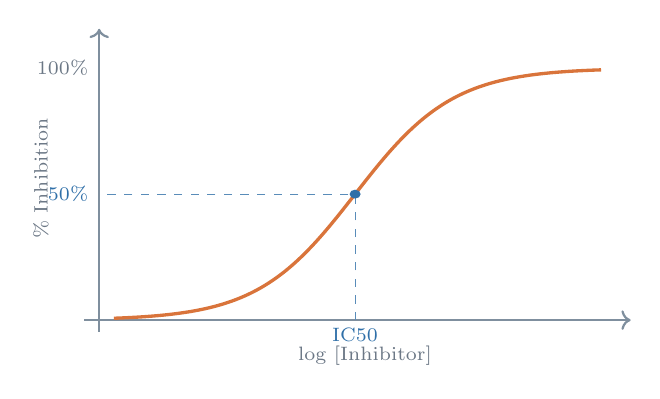
\begin{tikzpicture}[xscale=1.25,yscale=1.0]
        \draw[->,nxdark!55,thick] (-0.15,0) -- (5.4,0);
        \draw[->,nxdark!55,thick] (0,-0.15) -- (0,3.7);
        \node[lbl,below] at (2.7,-0.25) {\e{log [Inhibitor]}};
        \node[lbl,rotate=90,above] at (-0.45,1.8) {\e{\% Inhibition}};

        \draw[nxaccent,very thick] plot[domain=0.15:5.1,samples=90,smooth]
             (\x,{3.2/(1+exp(-2.0*(\x-2.6)))});

        \draw[dashed,nxblue!80] (2.6,0) -- (2.6,1.6) -- (0,1.6);
        \fill[nxblue] (2.6,1.6) circle (1.6pt);
        \node[lbl,text=nxblue,below] at (2.6,-0.02) {\e{IC50}};
        \node[lbl,text=nxblue,left]  at (-0.05,1.6) {\e{50\%}};
        \node[lbl,left] at (-0.05,3.2) {\e{100\%}};
      \end{tikzpicture}

      \vspace{2mm}
      {\footnotesize\color{nxgray}
       منحنی پاسخ به غلظت؛ \e{IC50} نقطه‌ی رسیدن به نیمه‌ی حداکثر مهار است.}
    \end{column}
  \end{columns}
  \note{این تمایز را حتماً بگو، چون از نظر علمی مهم است و نشان می‌دهد ادبیات را دقیق خوانده‌ای: \e{Kd} و \e{Ki} معیار اتصال‌اند، \e{IC50} معیار اثر عملکردی. ادبیات مقایسه‌ی ابزارهای \e{DTA} هم صراحتاً روی همین تأکید می‌کند.}
\end{frame}

%---------------------------------------------------------------- 8 --
\begin{frame}{جمع‌بندی معیارهای اتصال و مهار}
  \framesubtitle{کدام معیار چه چیزی را می‌سنجد؟}
  \vspace{3mm}
  \centering
  {\small
  \rowcolors{2}{nxlight}{white}
  \begin{tabular}{p{0.16\textwidth} p{0.34\textwidth} p{0.28\textwidth}}
    \rowcolor{nxdark}
    \thd{معیار} & \thd{مفهوم} & \thd{مقدار کمتر یعنی} \\
    \E{Kd}   & \e{Dissociation constant}        & \e{affinity} بیشتر \\
    \E{pKd}  & \e{−log\textsubscript{10}(K\textsubscript{d})} & \e{affinity} بیشتر \\
    \E{Ki}   & \e{Inhibition constant}          & \e{affinity} بیشتر \\
    \E{pKi}  & \e{−log\textsubscript{10}(K\textsubscript{i})} & \e{affinity} بیشتر \\
    \E{IC50} & غلظت لازم برای ۵۰٪ مهار          & \e{potency} بیشتر \\
  \end{tabular}}

  \vspace{5mm}
  \begin{exampleblock}{کاربرد در عمل}
    در بسیاری از \e{benchmark}های \e{DTA}، مقادیر \e{affinity} به شکل
    \key{لگاریتمی} مانند \e{pKd} یا \e{pKi} استفاده می‌شوند.
    برای نمونه \e{DCGAN-DTA} روی \e{BindingDB} مقادیر را به \e{pKd} تبدیل کرده
    و \e{PDBBind} نیز شامل مقادیر \e{log-transformed} از \e{Ki} و \e{Kd} است.
  \end{exampleblock}
  \note{این اسلاید پل به بخش بعد است. بگو: «پس برچسبی که مدل‌ها پیش‌بینی می‌کنند معمولاً یک عدد پیوسته در مقیاس لگاریتمی است؛ حالا ببینیم پژوهشگران برای پیش‌بینی این عدد چه مسیری را طی کرده‌اند.»}
\end{frame}

%======================================================================
\section{مسیر پژوهشی}
%======================================================================

%---------------------------------------------------------------- 9 --
\begin{frame}{درخت تکاملی روش‌های پیش‌بینی \e{DTA}}
  \framesubtitle{از ۲۰۱۵ تا ۲۰۲۶ --- بر پایه‌ی مرور \e{Wang et al.}, \e{Biotechnology Advances}, ۲۰۲۶}
  \vspace{1mm}
  \centering
  \begin{tikzpicture}[x=1mm,y=1mm,
      tn/.style={nxn,minimum height=6.6mm,inner xsep=3pt,inner ysep=1.5pt,
                 font=\tiny,align=center},
      bus/.style={draw=nxdark!65,thick},
      dn/.style={-{Stealth[length=1.8mm,width=1.4mm]},draw=nxdark!65,thick}]

    % ---- tier A: the historical spine --------------------------------
    \node[tn,ghost,minimum width=34mm] (a1) at (22,27)  {\fa{شباهت و \e{Kernel}}\\\e{KronRLS} --- ۲۰۱۵};
    \node[tn,ghost,minimum width=34mm] (a2) at (64,27)  {\fa{یادگیری ماشین ویژگی‌محور}\\\e{SimBoost} --- ۲۰۱۷};
    \node[tn,model,minimum width=34mm] (a3) at (106,27) {\fa{یادگیری عمیق}\\\e{DeepDTA} --- ۲۰۱۸};
    \draw[dn] (a1)--(a2); \draw[dn] (a2)--(a3);

    % ---- tier B: three representation families -----------------------
    \node[tn,minimum width=34mm] (b1) at (22,12)  {\fa{توالی و} \e{CNN}\\\e{DeepDTA} $\cdot$ \e{WideDTA}};
    \node[tn,minimum width=34mm] (b2) at (64,12)  {\fa{گراف و} \e{GNN}\\\e{GraphDTA} $\cdot$ \e{MGraphDTA}};
    \node[tn,minimum width=34mm] (b3) at (106,12) {\fa{توجه و} \e{Transformer}\\\e{AttentionDTA} $\cdot$ \e{ELECTRA-DTA}};
    \draw[bus] (a3.south) -- (106,20);
    \draw[bus] (22,20) -- (106,20);
    \draw[dn] (22,20) -- (b1.north);
    \draw[dn] (64,20) -- (b2.north);
    \draw[dn] (106,20) -- (b3.north);

    % ---- tier C: representation learning -----------------------------
    \node[tn,model,minimum width=66mm] (rep) at (64,0)
      {\fa{یادگیری نمایش} --- \e{Representation Learning}};
    \draw[bus] (b1.south) -- (22,5.5);
    \draw[bus] (b2.south) -- (64,5.5);
    \draw[bus] (b3.south) -- (106,5.5);
    \draw[bus] (22,5.5) -- (106,5.5);
    \draw[dn] (64,5.5) -- (rep.north);

    % ---- tier D: three sibling branches of representation learning ---
    \node[tn,minimum width=34mm] (d1) at (22,-13)  {\fa{ترکیب چندوجهی}\\\e{Fusion} $\cdot$ \e{Multimodal}};
    \node[tn,res,minimum width=34mm,draw=nxaccent,line width=0.7pt] (d2) at (64,-13)
      {\fa{یادگیری نمایش مولد}\\\e{Generative}};
    \node[tn,minimum width=34mm] (d3) at (106,-13) {\fa{پیش‌آموزش‌دیده}\\\e{Protein} \& \e{Chemical LM}};
    \draw[bus] (rep.south) -- (64,-7);
    \draw[bus] (22,-7) -- (106,-7);
    \draw[dn] (22,-7) -- (d1.north);
    \draw[dn] (64,-7) -- (d2.north);
    \draw[dn] (106,-7) -- (d3.north);

    % ---- tier E: the two papers this thesis studies -------------------
    \node[tn,minimum width=32mm,fill=nxblue!25,draw=nxblue,line width=0.7pt,
          font=\tiny\bfseries] (e1) at (44,-27) {\e{GAN} $\rightarrow$ \e{DCGAN-DTA} --- ۲۰۲۴};
    \node[tn,minimum width=32mm,fill=nxteal!25,draw=nxteal,line width=0.7pt,
          font=\tiny\bfseries] (e2) at (84,-27) {\e{VAE} $\rightarrow$ \e{Co-VAE} --- ۲۰۲۲};
    \draw[bus] (d2.south) -- (64,-20);
    \draw[bus] (44,-20) -- (84,-20);
    \draw[dn] (44,-20) -- (e1.north);
    \draw[dn] (84,-20) -- (e2.north);
  \end{tikzpicture}

  \vspace{1mm}
  {\scriptsize\color{nxgray}
   هر شاخه پاسخی به یک محدودیت متفاوت است --- \key{نه جانشین کامل نسل قبلی}.
   دو برگ پررنگ، نقطه‌ی ورود این پایان‌نامه‌اند.}
  \note{مهم‌ترین اسلاید بخش دوم؛ حدود دو تا سه دقیقه رویش وقت بگذار. دو پیام اصلی: (۱) این یک زنجیره‌ی خطی نیست، یک درخت است و شاخه‌های پایینی هم‌زمان‌اند نه پشت سر هم؛ (۲) \e{Generative} یک شاخه‌ی هم‌رده‌ی \e{Fusion} و \e{Pre-trained} است، نه مرحله‌ی بعد از \e{GNN}. در پایان انگشت بگذار روی دو برگ پررنگ و بگو «پایان‌نامه دقیقاً اینجاست».}
\end{frame}

%--------------------------------------------------------------- 10 --
\begin{frame}{مرحله‌ی اول: شباهت و \e{Kernel}}
  \framesubtitle{\e{KronRLS} --- \e{Pahikkala et al.}, ۲۰۱۵}
  \vspace{2mm}
  \begin{columns}[T]
    \begin{column}{0.50\textwidth}
      \small
      \begin{block}{فرض اصلی این نسل}
        اگر دو دارو از نظر شیمیایی شبیه باشند، احتمالاً \e{affinity} مشابهی
        دارند؛ پروتئین‌های مشابه نیز الگوی \e{binding} مشابهی دارند.
      \end{block}

      \vspace{1mm}
      \begin{exampleblock}{\e{KronRLS}}
        \small
        \e{Kronecker Regularized Least Squares} --- شباهت دارو--دارو و
        هدف--هدف را ترکیب می‌کند و مسئله را در قالب
        \e{regularized least squares} حل می‌کند.
      \end{exampleblock}
    \end{column}

    \begin{column}{0.46\textwidth}
      \centering
      \begin{tikzpicture}[x=1mm,y=1mm,font=\scriptsize]
        \node[drug,minimum width=25mm]  (s1) at (0,14)   {\fa{شباهت دارو}};
        \node[targ,minimum width=25mm]  (s2) at (30,14)  {\fa{شباهت پروتئین}};
        \node[model,minimum width=36mm] (k)  at (15,2)   {\e{Kernel} / \e{KronRLS}};
        \node[res,minimum width=25mm]   (a)  at (15,-11) {\e{Affinity}};
        \draw[arr] (s1)--(k); \draw[arr] (s2)--(k); \draw[arr] (k)--(a);
      \end{tikzpicture}

      \vspace{2mm}
      \begin{alertblock}{محدودیت}
        \small مدل فقط به اندازه‌ی کیفیت \e{similarity}ای که \key{انسان}
        تعریف کرده خوب بود؛ نمایش هنوز دستی و از پیش تعریف‌شده است.
      \end{alertblock}
    \end{column}
  \end{columns}
  \note{کوتاه رد شو. پیام: کیفیت مدل عملاً برابر بود با کیفیت تابع شباهتی که انسان تعریف می‌کرد. \e{KronRLS} هنوز هم یکی از \e{baseline}های استاندارد است و \e{DeepDTA} مستقیماً با آن مقایسه می‌شود.}
\end{frame}

%--------------------------------------------------------------- 11 --
\begin{frame}{مرحله‌ی دوم: یادگیری ماشین ویژگی‌محور}
  \framesubtitle{\e{SimBoost} --- \e{He et al.}, ۲۰۱۷}
  \vspace{2mm}
  \begin{columns}[T]
    \begin{column}{0.48\textwidth}
      \small
      \begin{block}{ویژگی‌های صریح به جای شباهت صرف}
        \begin{itemize}\itemsep0.2ex
          \item دارو: \e{fingerprints}، \e{descriptors}، ویژگی‌های ساختاری دوبعدی
          \item پروتئین: شباهت توالی، ویژگی‌های فیزیکوشیمیایی، اطلاعات تکاملی
          \item جفت دارو--هدف: ویژگی‌های شبکه‌ای
        \end{itemize}
      \end{block}

      \vspace{1mm}
      {\footnotesize
       \e{SimBoost} به جای \e{kernel} ساده از \E{Gradient Boosting Machines}
       استفاده کرد و توانست روابط \key{غیرخطی‌تر} را مدل کند.}
    \end{column}

    \begin{column}{0.48\textwidth}
      \centering
      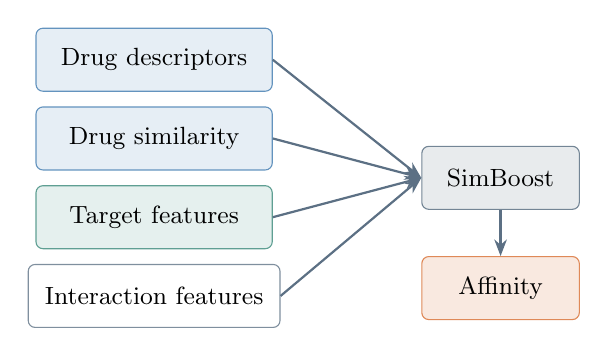
\begin{tikzpicture}[x=1mm,y=1mm,font=\scriptsize]
        \node[drug,minimum width=30mm]  (f1) at (0,16)  {\e{Drug descriptors}};
        \node[drug,minimum width=30mm]  (f2) at (0,6)   {\e{Drug similarity}};
        \node[targ,minimum width=30mm]  (f3) at (0,-4)  {\e{Target features}};
        \node[nxn,minimum width=30mm]   (f4) at (0,-14) {\e{Interaction features}};
        \node[model,minimum width=20mm] (sb) at (44,1)  {\e{SimBoost}};
        \node[res,minimum width=20mm]   (af) at (44,-13) {\e{Affinity}};
        \draw[arr] (f1.east) -- (sb.west);
        \draw[arr] (f2.east) -- (sb.west);
        \draw[arr] (f3.east) -- (sb.west);
        \draw[arr] (f4.east) -- (sb.west);
        \draw[arr] (sb) -- (af);
      \end{tikzpicture}

      \vspace{2mm}
      \begin{alertblock}{گلوگاه جابه‌جا شد}
        \small از \e{Similarity Engineering} به \key{\e{Feature Engineering}} ---
        ولی هنوز انسان در حلقه است.
      \end{alertblock}
    \end{column}
  \end{columns}
  \note{پیام کوتاه: پیشرفت واقعی بود (مدل‌سازی غیرخطی)، ولی گلوگاه فقط یک قدم عقب‌تر رفت. این همان چیزی است که یادگیری عمیق در مرحله‌ی بعد حذفش می‌کند.}
\end{frame}

%--------------------------------------------------------------- 12 --
\begin{frame}{مرحله‌ی سوم: ورود یادگیری عمیق}
  \framesubtitle{\e{DeepDTA} --- \e{Öztürk et al.}, ۲۰۱۸ \quad$\cdot$\quad \e{WideDTA}, ۲۰۱۹}
  \vspace{2mm}
  \centering
  \begin{tikzpicture}[x=1mm,y=1mm,font=\scriptsize]
    \node[drug,minimum width=24mm]  (sm) at (12,10)  {\e{Drug SMILES}};
    \node[targ,minimum width=24mm]  (pr) at (12,-8)  {\e{Protein sequence}};
    \node[nxn,minimum width=20mm]   (e1) at (42,10)  {\e{Embedding}};
    \node[nxn,minimum width=20mm]   (e2) at (42,-8)  {\e{Embedding}};
    \node[model,minimum width=20mm] (c1) at (68,10)  {\e{1D CNN}};
    \node[model,minimum width=20mm] (c2) at (68,-8)  {\e{1D CNN}};
    \node[model,minimum width=18mm] (fu) at (94,1)   {\e{Fusion}};
    \node[res,minimum width=18mm]   (af) at (117,1)  {\e{Affinity}};
    \draw[arr] (sm)--(e1); \draw[arr] (e1)--(c1);
    \draw[arr] (pr)--(e2); \draw[arr] (e2)--(c2);
    \draw[arr] (c1.east) -- (fu.north west);
    \draw[arr] (c2.east) -- (fu.south west);
    \draw[arr] (fu)--(af);
  \end{tikzpicture}

  \vspace{3mm}
  \begin{columns}[T]
    \begin{column}{0.48\textwidth}
      \begin{alertblock}{تغییر بنیادی}
        \small
        نمایش دیگر به‌طور کامل توسط انسان تعریف نمی‌شود؛
        \key{شبکه آن را از داده‌ی خام یاد می‌گیرد}.
      \end{alertblock}
    \end{column}
    \begin{column}{0.48\textwidth}
      \begin{exampleblock}{\e{WideDTA} --- گام بعدی}
        \small
        افزودن \e{protein domains/motifs} و
        \e{maximum common substructure} برای نمایشی غنی‌تر.
      \end{exampleblock}
    \end{column}
  \end{columns}
  \note{\e{DeepDTA} نقطه‌ی عطف این حوزه است و تقریباً همه‌ی مقالات بعدی با آن مقایسه می‌شوند. اگر وقت کم بود، فقط همین اسلاید را از کل بخش بگو.}
\end{frame}

%--------------------------------------------------------------- 13 --
\begin{frame}{مرحله‌ی چهارم: گراف و نمایش ساختارآگاه}
  \framesubtitle{\e{GraphDTA} --- \e{Nguyen et al.}, ۲۰۲۱}
  \vspace{2mm}
  \begin{columns}[T]
    \begin{column}{0.50\textwidth}
      \centering
      \begin{tikzpicture}[x=1mm,y=1mm,font=\scriptsize]
        \node[drug,minimum width=26mm]  (d)  at (0,18)  {\e{Drug}};
        \node[nxn,minimum width=26mm]   (g)  at (0,7)   {\e{Molecular graph}};
        \node[model,minimum width=26mm] (gn) at (0,-4)  {\e{GNN}};
        \node[targ,minimum width=26mm]  (p)  at (40,18) {\e{Protein sequence}};
        \node[model,minimum width=26mm] (cn) at (40,7)  {\e{CNN}};
        \node[model,minimum width=20mm] (fu) at (20,-15) {\e{Fusion}};
        \node[res,minimum width=20mm]   (af) at (20,-26) {\e{Affinity}};
        \draw[arr] (d)--(g); \draw[arr] (g)--(gn);
        \draw[arr] (p)--(cn);
        \draw[arr] (gn.south) -- (fu.north west);
        \draw[arr] (cn.south) -- (fu.north east);
        \draw[arr] (fu)--(af);
      \end{tikzpicture}
    \end{column}

    \begin{column}{0.46\textwidth}
      \small
      \begin{block}{چرا گراف؟}
        \e{SMILES} فقط یک \key{سریال‌سازی} از مولکول است، در حالی که مولکول
        ذاتاً یک گراف است: اتم $\rightarrow$ \e{Node}، پیوند $\rightarrow$ \e{Edge}.
      \end{block}

      \vspace{1mm}
      {\footnotesize
       \e{GraphDTA} چند معماری را بررسی کرد:
       \e{GCN} $\cdot$ \e{GAT} $\cdot$ \e{GAT-GCN} $\cdot$ \e{GIN}.}

      \vspace{2mm}
      \begin{exampleblock}{نتیجه}
        \small مسئله فقط عمیق‌تر کردن شبکه نبود؛ \key{نوع نمایش} هم تغییر کرد:
        از \e{sequence representation} به \e{structure-aware representation}.
      \end{exampleblock}
    \end{column}
  \end{columns}
  \note{اگر پرسیده شد چرا گراف بهتر است: چون اطلاعات ساختاری (حلقه‌ها، شاخه‌ها، همسایگی اتم‌ها) در \e{SMILES} به‌صورت ضمنی و در گراف به‌صورت صریح کد می‌شود. وارد جزئیات \e{GNN} نشو، موضوع پایان‌نامه نیست.}
\end{frame}

%--------------------------------------------------------------- 14 --
\begin{frame}{مرحله‌ی پنجم: توجه و \e{Transformer}}
  \framesubtitle{\e{AttentionDTA} $\cdot$ \e{ELECTRA-DTA} $\cdot$ \e{FusionDTA}, ۲۰۲۲}
  \vspace{2mm}
  \begin{columns}[T]
    \begin{column}{0.48\textwidth}
      \small
      \begin{block}{پرسش تازه}
        حتی با نمایش خوب، هنوز باید مشخص شود \key{کدام بخش} از دارو و
        کدام بخش از پروتئین برای \e{binding} مهم‌تر است.
      \end{block}

      \vspace{1mm}
      \begin{exampleblock}{\e{FusionDTA}}
        \small
        تمرکز بر \e{feature aggregation} با
        \e{attention-based feature polymerization} و
        \e{knowledge distillation}.
      \end{exampleblock}
    \end{column}

    \begin{column}{0.48\textwidth}
      \centering
      \vspace{1mm}
      \begin{tikzpicture}[x=1mm,y=1mm,font=\scriptsize]
        \node[drug,minimum width=22mm]  (d) at (0,12)  {\e{Drug tokens}};
        \node[targ,minimum width=22mm]  (p) at (0,-4)  {\e{Protein tokens}};
        \node[model,minimum width=30mm] (at) at (36,4) {\e{Attention} / \e{Transformer}};
        \node[res,minimum width=26mm]   (af) at (36,-12) {\e{Affinity}};
        \draw[arr] (d.east) -- (at.north west);
        \draw[arr] (p.east) -- (at.south west);
        \draw[arr] (at)--(af);
      \end{tikzpicture}

      \vspace{2mm}
      {\footnotesize\color{nxgray}
       \e{CNN} برای الگوهای \e{local} مناسب است؛ \e{attention} می‌تواند
       وابستگی‌های دوربرد و میان‌وجهی را مدل کند.}
    \end{column}
  \end{columns}

  \vspace{1mm}
  \centering
  {\footnotesize
   تمرکز از «چه ویژگی‌ای استخراج کنیم؟» به
   \key{«چگونه ویژگی‌ها را با هم تعامل دهیم؟»} منتقل شد.}
  \note{این مرحله در نسخه‌ی قبلی ارائه غایب بود. نکته‌ی کلیدی: \e{attention} یک نوع نمایش جدید نمی‌سازد، بلکه نحوه‌ی ترکیب نمایش‌های موجود را یاد می‌گیرد.}
\end{frame}

%--------------------------------------------------------------- 15 --
\begin{frame}{مرحله‌ی ششم: چندوجهی و مدل‌های پیش‌آموزش‌دیده}
  \framesubtitle{\e{Multi-modal fusion} و \e{Protein/Chemical Language Models}}
  \vspace{2mm}
  \begin{columns}[T]
    \begin{column}{0.44\textwidth}
      \small
      \begin{block}{یک نمایش کافی نیست}
        \begin{itemize}\itemsep0.2ex
          \item دارو: \e{SMILES}، گراف مولکولی، \e{descriptors}
          \item پروتئین: توالی، ساختار، \e{binding site}، اطلاعات تکاملی
        \end{itemize}
      \end{block}

      \vspace{1mm}
      {\footnotesize
       نمونه‌ها: \e{DeepFusionDTA} $\cdot$ \e{MDF-DTA} $\cdot$
       \e{PocketDTA} $\cdot$ \e{GraphTransDTA}}
    \end{column}

    \begin{column}{0.52\textwidth}
      \centering
      \begin{tikzpicture}[x=1mm,y=1mm,font=\scriptsize]
        \node[targ,minimum width=28mm]  (ps) at (0,14)  {\e{Protein sequence}};
        \node[model,minimum width=28mm] (pl) at (0,3)   {\e{Pre-trained Protein LM}};
        \node[drug,minimum width=28mm]  (ds) at (0,-12) {\e{Drug SMILES}};
        \node[model,minimum width=28mm] (ml) at (0,-23) {\e{Molecular LM}};
        \node[model,minimum width=26mm] (cx) at (46,-10) {\e{Cross-modal}\\\e{interaction}};
        \node[res,minimum width=20mm]   (af) at (46,-24) {\e{Affinity}};
        \draw[arr] (ps)--(pl); \draw[arr] (ds)--(ml);
        \draw[arr] (pl.east) -- (cx.north west);
        \draw[arr] (ml.east) -- (cx.south west);
        \draw[arr] (cx)--(af);
      \end{tikzpicture}

      \vspace{1mm}
      {\footnotesize\color{nxgray}
       \e{ESM} $\cdot$ \e{ProtBERT} $\cdot$ \e{ChemBERT} --- در مرور ۲۰۲۶،
       مدل‌های پیش‌آموزش‌دیده یک \key{پارادایم مستقل} شمرده می‌شوند.}
    \end{column}
  \end{columns}
  \note{این مرحله هم در نسخه‌ی قبلی غایب بود و اضافه‌کردنش نشان می‌دهد ادبیات را تا ۲۰۲۶ دنبال کرده‌ای. اگر استاد پرسید چرا از این مسیر استفاده نکرده‌ای، بگو موضوع پایان‌نامه شاخه‌ی مولد است و این شاخه‌ی موازی می‌تواند کار آینده باشد.}
\end{frame}

%--------------------------------------------------------------- 16 --
\begin{frame}{مرحله‌ی هفتم: یادگیری نمایش مولد}
  \framesubtitle{شاخه‌ای هم‌رده با \e{Fusion} و \e{Pre-trained} --- نه مرحله‌ی بعد از \e{GNN}}
  \vspace{2mm}
  \begin{columns}[T]
    \begin{column}{0.46\textwidth}
      \small
      \begin{block}{پرسش این شاخه}
        تا اینجا مدل‌ها یک نمایش می‌گیرند و \e{affinity} را پیش‌بینی می‌کنند.
        پرسش تازه: آیا می‌توان از \key{مدل‌های مولد} برای یادگیری
        \key{نمایش بهتر} استفاده کرد؟
      \end{block}

      \vspace{1mm}
      \begin{alertblock}{چرا این شاخه مهم است}
        \small
        \begin{itemize}\itemsep0.2ex
          \item بهره‌گیری از داده‌ی \key{بدون برچسب}
          \item فضای نهان ساختارمند و پیوسته
          \item امکان \e{pretraining} پیش از رگرسیون
        \end{itemize}
      \end{alertblock}
    \end{column}

    \begin{column}{0.50\textwidth}
      \centering
      \vspace{1mm}
      \begin{tikzpicture}[x=1mm,y=1mm,font=\scriptsize]
        \node[res,minimum width=40mm,draw=nxaccent,line width=0.7pt] (gm) at (30,16)
          {\fa{یادگیری نمایش مولد}};
        \node[nxn,minimum width=20mm,fill=nxblue!12,draw=nxblue!75] (gan) at (8,2)  {\E{GAN}};
        \node[nxn,minimum width=20mm,fill=nxteal!12,draw=nxteal!75] (vae) at (52,2) {\E{VAE}};
        \node[nxn,minimum width=26mm,fill=nxblue!25,draw=nxblue,font=\scriptsize\bfseries]
          (dc) at (8,-13) {\e{DCGAN-DTA}};
        \node[nxn,minimum width=26mm,fill=nxteal!25,draw=nxteal,font=\scriptsize\bfseries]
          (cv) at (52,-13) {\e{Co-VAE}};
        \draw[arr] (gm)--(gan); \draw[arr] (gm)--(vae);
        \draw[arr] (gan)--(dc); \draw[arr] (vae)--(cv);
        \node[lbl,text width=26mm,align=center] at (8,-23)  {\fa{یادگیری تخاصمی}};
        \node[lbl,text width=26mm,align=center] at (52,-23) {\fa{یادگیری وردشی}};
      \end{tikzpicture}
    \end{column}
  \end{columns}
  \note{اینجا پل اصلی ارائه است. جمله‌ی گذار: «این دو مقاله دو پاسخ متفاوت به یک پرسش واحدند؛ حالا هر کدام را جداگانه می‌بینیم.» حتماً تأکید کن که \e{Generative} از نظر تاریخی بعد از \e{GNN} نیامده، بلکه یک شاخه‌ی موازی است.}
\end{frame}

%--------------------------------------------------------------- 17 --
\begin{frame}{افق کنونی: ۲۰۲۶}
  \framesubtitle{\e{Foundation} $\cdot$ \e{Multimodal} $\cdot$ \e{Task-adaptive} $\cdot$ \e{Cold-start}}
  \vspace{3mm}
  \begin{columns}[T]
    \begin{column}{0.48\textwidth}
      \small
      \begin{block}{مسیرهای فعال امروز}
        \begin{itemize}\itemsep0.25ex
          \item نمایش‌های \e{pre-trained} در مقیاس بزرگ
          \item یادگیری \e{multimodal} (توالی + گراف + ساختار)
          \item \e{cross-modal interaction} به جای الحاق ساده
          \item تعمیم در شرایط \e{cold-start}
          \item \e{meta-learning} و \e{task adaptation}
          \item مدل‌های \e{binding-site-aware}
        \end{itemize}
      \end{block}
    \end{column}

    \begin{column}{0.48\textwidth}
      \vspace{1mm}
      \begin{exampleblock}{نمونه‌های ۲۰۲۶}
        \small
        \begin{itemize}\itemsep0.25ex
          \item \lr{A meta learning and task adaptive approach for DTA
                --- Nature Communications}
          \item \e{DCI-SiteDTA} --- ورود اطلاعات \e{binding site}
          \item \e{GraphTransDTA} --- \e{Graph Transformer} برای
                ترکیب داده‌های چندوجهی
        \end{itemize}
      \end{exampleblock}

      \vspace{1mm}
      {\footnotesize\color{nxgray}
       نکته‌ی مهم: \key{مسیر متوقف نشده}. شاخه‌ی مولد یکی از چند مسیر فعال است
       و این پایان‌نامه دقیقاً همان شاخه را بررسی می‌کند.}
    \end{column}
  \end{columns}
  \note{این اسلاید نشان می‌دهد که تصویر کاملی از حوزه داری و می‌دانی پایان‌نامه‌ات کجای آن می‌نشیند. اگر استاد پرسید «چرا سراغ \e{foundation models} نرفتی؟» بگو منابع محاسباتی و دامنه‌ی پایان‌نامه محدود است و این مسیر را به‌عنوان کار آینده مطرح می‌کنم.}
\end{frame}

%--------------------------------------------------------------- 18 --
\begin{frame}{جایگاه پایان‌نامه در این درخت}
  \framesubtitle{چرا دقیقاً این دو مقاله؟}
  \vspace{2mm}
  \centering
  \begin{tikzpicture}[x=1mm,y=1mm,font=\scriptsize,
      dn/.style={-{Stealth[length=1.9mm,width=1.5mm]},draw=nxdark!65,thick},
      bus/.style={draw=nxdark!65,thick}]
    \node[model,minimum width=28mm,minimum height=7mm] (dl)  at (64,18) {\fa{یادگیری عمیق}};
    \node[model,minimum width=44mm,minimum height=7mm] (rep) at (64,7)  {\e{Representation Learning}};
    \draw[dn] (dl)--(rep);

    \node[ghost,minimum width=17mm,minimum height=7mm] (s1) at (12,-7)  {\fa{توالی}};
    \node[ghost,minimum width=17mm,minimum height=7mm] (s2) at (33,-7)  {\fa{گراف}};
    \node[ghost,minimum width=17mm,minimum height=7mm] (s3) at (54,-7)  {\fa{توجه}};
    \node[ghost,minimum width=19mm,minimum height=7mm] (s4) at (77,-7)  {\fa{چندوجهی}};
    \node[res,minimum width=22mm,minimum height=7mm,draw=nxaccent,line width=0.7pt]
      (s5) at (105,-7) {\fa{مولد}};
    \draw[bus] (rep.south) -- (64,-1);
    \draw[bus] (12,-1) -- (105,-1);
    \foreach \n/\x in {s1/12,s2/33,s3/54,s4/77,s5/105} \draw[dn] (\x,-1) -- (\n.north);

    \node[nxn,minimum width=30mm,minimum height=7mm,fill=nxblue!25,draw=nxblue,
          line width=0.7pt,font=\scriptsize\bfseries] (dc) at (72,-22)
      {\e{GAN} $\rightarrow$ \e{DCGAN-DTA}};
    \node[nxn,minimum width=26mm,minimum height=7mm,fill=nxteal!25,draw=nxteal,
          line width=0.7pt,font=\scriptsize\bfseries] (cv) at (108,-22)
      {\e{VAE} $\rightarrow$ \e{Co-VAE}};
    \draw[bus] (s5.south) -- (105,-15);
    \draw[bus] (72,-15) -- (108,-15);
    \draw[dn] (72,-15) -- (dc.north);
    \draw[dn] (108,-15) -- (cv.north);
  \end{tikzpicture}

  \vspace{1mm}
  \begin{alertblock}{صورت‌بندی قابل دفاع}
    \centering
    \small
    این پژوهش ادعا نمی‌کند روش‌های پیشین ضعیف بوده‌اند؛ بلکه بر
    \key{شاخه‌ی یادگیری نمایش مولد} در تکامل روش‌های \e{DTA} تمرکز می‌کند و
    دو نماینده‌ی اصلی آن را زیر یک پروتکل مشترک مقایسه می‌کند.
  \end{alertblock}
  \note{این اسلاید پاسخ آماده به پرسش «چرا این دو مقاله؟» است. جمله‌ای که نباید بگویی: «روش‌های قبلی ضعیف بودند و من مدل بهتری می‌سازم» --- چون اثباتش نیازمند آزمایش گسترده است. جمله‌ای که باید بگویی: «این دو، نماینده‌های شاخص دو زیرشاخه‌ی یک پارادایم‌اند و تاکنون زیر یک پروتکل مشترک مقایسه نشده‌اند.»}
\end{frame}

%======================================================================
\section{مقاله‌ی اول: \e{DCGAN-DTA}}
%======================================================================

%--------------------------------------------------------------- 15 --
\begin{frame}{\e{DCGAN-DTA}}
  \framesubtitle{نماینده‌ی شاخه‌ی \e{GAN} \ --- \ \e{Kalemati et al.}, \e{BMC Genomics}, ۲۰۲۴}
  \vspace{2mm}
  \begin{columns}[T]
    \begin{column}{0.48\textwidth}
      \small
      \begin{alertblock}{چالش‌های مورد اشاره‌ی نویسندگان}
        \begin{itemize}\itemsep0.2ex
          \item داده‌ی آموزشی محدود (\e{limited training data})
          \item انتخاب و مهندسی ویژگی
          \item نیاز به اعتبارسنجی قوی‌تر
          \item \e{generalization} به داده‌های دیده‌نشده
        \end{itemize}
      \end{alertblock}

      \vspace{1mm}
      \centering
      \begin{tikzpicture}[node distance=5mm,font=\footnotesize]
        \node[model,minimum width=22mm] (g) {\e{Generator}};
        \node[model,minimum width=22mm,right=8mm of g] (d) {\e{Discriminator}};
        \draw[arr] (g) -- (d);
        \draw[arr,dashed] (d.south) .. controls +(0,-7mm) and +(0,-7mm) .. (g.south)
          node[lbl,midway,below] {\fa{سیگنال تخاصمی}};
      \end{tikzpicture}
    \end{column}

    \begin{column}{0.48\textwidth}
      \small
      \begin{block}{ایده}
        استفاده از \E{Deep Convolutional Generative Adversarial Network}
        برای \key{یادگیری نمایش} دارو و پروتئین.
      \end{block}

      \vspace{1mm}
      \begin{exampleblock}{چرا این مقاله مهم است}
        \footnotesize
        \e{DCGAN-DTA} را نباید «یک مدل \e{CNN} دیگر» دید. اهمیت آن در این است که
        ظرفیت \key{یادگیری نمایشِ} مدل‌های مولد را وارد مسئله‌ی \e{DTA} می‌کند و از
        \key{\e{pretraining}} --- از جمله روی داده‌ی بدون برچسب --- برای استخراج
        نمایش بهره می‌گیرد.
      \end{exampleblock}
    \end{column}
  \end{columns}
  \note{جمله‌ی کلیدی این اسلاید: «\e{DCGAN-DTA} تلاش می‌کند ظرفیت یادگیری نمایش مدل‌های مولد را وارد مسئله‌ی \e{DTA} کند و از \e{pretraining} برای استخراج نمایش استفاده کند.» حتماً تأکید کن که \e{GAN} اینجا برای تولید دارو به کار نمی‌رود، بلکه برای یادگیری نمایش --- این تفاوت ظریف ولی مهمی است و معمولاً همین‌جا سؤال می‌شود.}
\end{frame}

%--------------------------------------------------------------- 16 --
\begin{frame}{معماری \e{DCGAN-DTA}}
  \framesubtitle{نمودار بلوکی مقاله --- \e{Kalemati et al.}, \e{BMC Genomics}, ۲۰۲۴}
  \vspace{1mm}
  \begin{columns}[c]
    \begin{column}{0.40\textwidth}
      \centering
      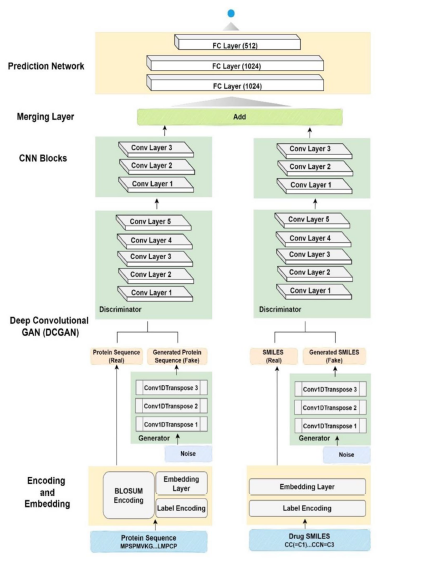
\includegraphics[width=0.96\linewidth]{presentation-figs/DCGAN-block-diagram.png}
    \end{column}

    \begin{column}{0.57\textwidth}
      \begin{block}{پنج مرحله --- شکل از پایین به بالا خوانده می‌شود}
        \footnotesize
        \begin{enumerate}\itemsep0.35ex
          \item کدگذاری و تعبیه --- \e{Label} / \e{BLOSUM} + \e{Embedding}
          \item پیش‌آموزش \e{DCGAN} --- \e{Generator} + \e{Discriminator}
          \item بلوک‌های \e{CNN} --- استخراج ویژگی
          \item لایه‌ی ادغام دو شاخه --- \e{Add}
          \item شبکه‌ی پیش‌بینی --- \e{FC 1024} $\rightarrow$ \e{512}
        \end{enumerate}
      \end{block}

      \vspace{1mm}
      \begin{alertblock}{نکته‌ی کلیدی}
        \footnotesize
        \e{GAN} اینجا \key{برای تولید دارو نیست}؛ \e{Generator} و
        \e{Discriminator} فقط برای \key{پیش‌آموزش نمایش} به کار می‌روند و
        نمایش آموخته‌شده به سر رگرسیون داده می‌شود.
      \end{alertblock}
    \end{column}
  \end{columns}
  \note{شکل را از پایین به بالا توضیح بده --- همان ترتیبی که در ستون کنارش شماره خورده است. دو شاخه‌ی چپ و راست شکل کاملاً متقارن‌اند؛ تنها تفاوت جدی، \e{BLOSUM encoding} در شاخه‌ی پروتئین است که اطلاعات تکاملی (شباهت جانشینی اسیدهای آمینه) را وارد مدل می‌کند. اگر وقت کم بود فقط بگو: کدگذاری، پیش‌آموزش تخاصمی، \e{CNN}، ادغام، رگرسیون.}
\end{frame}

%======================================================================
\section{مقاله‌ی دوم: \e{Co-VAE}}
%======================================================================

%--------------------------------------------------------------- 17 --
\begin{frame}{\e{Co-VAE}}
  \framesubtitle{نماینده‌ی شاخه‌ی \e{VAE} \ --- \ \e{Li, Zhao \& Li}, \e{IEEE TPAMI}, ۲۰۲۲}
  \vspace{3mm}
  \begin{columns}[T]
    \begin{column}{0.50\textwidth}
      \centering
      \begin{tikzpicture}[node distance=5mm,font=\footnotesize]
        \node[drug,minimum width=26mm] (d) {\e{Drug SMILES}};
        \node[model,minimum width=18mm,below=6mm of d] (v1) {\lr{$\text{VAE}_1$}};
        \node[nxn,minimum width=26mm,below=6mm of v1] (dl) {\e{Drug latent}};
        \draw[arr] (d)--(v1); \draw[arr] (v1)--(dl);

        \node[targ,minimum width=26mm,right=10mm of d] (t) {\e{Protein sequence}};
        \node[model,minimum width=18mm,below=6mm of t] (v2) {\lr{$\text{VAE}_2$}};
        \node[nxn,minimum width=26mm,below=6mm of v2] (tl) {\e{Target latent}};
        \draw[arr] (t)--(v2); \draw[arr] (v2)--(tl);

        \node[model,minimum width=34mm,below=8mm of $(dl)!0.5!(tl)$] (co) {\e{Co-regularization}};
        \node[res,minimum width=30mm,below=6mm of co] (af) {\e{Binding affinity}};
        \draw[arr] (dl.south) -- (co.north west);
        \draw[arr] (tl.south) -- (co.north east);
        \draw[arr] (co) -- (af);
      \end{tikzpicture}
    \end{column}

    \begin{column}{0.46\textwidth}
      \small
      \vspace{2mm}
      \begin{block}{ایده‌ی اصلی}
        دو \e{VAE} مجزا برای دارو و هدف، به‌همراه یک بخش
        \key{\e{co-regularization}} که فضاهای نهان را به مقدار
        \e{affinity} گره می‌زند.
      \end{block}

      \vspace{1.5mm}
      \begin{exampleblock}{چرا این مقاله مهم است}
        \footnotesize
        فضای نهان اینجا \key{احتمالاتی} است، نه یک بردار ثابت؛ و مدل فقط برای
        \e{prediction} طراحی نشده --- نویسندگان نشان می‌دهند می‌توان از آن برای
        \key{تولید داروهای جدید با هدف‌های مشابه} نیز استفاده کرد.
      \end{exampleblock}
    \end{column}
  \end{columns}
  \note{تفاوت بنیادی با مقاله‌ی قبل: آنجا نمایش با فرایند تخاصمی و در یک مرحله‌ی پیش‌آموزشِ جدا ساخته می‌شود؛ اینجا فضای نهان احتمالاتی است و بازسازی، هم‌تنظیمی و رگرسیون هم‌زمان آموزش می‌بینند. همین تقابل --- \e{Adversarial} در برابر \e{Variational} --- است که مقایسه‌ی این دو را برای پایان‌نامه ارزشمند می‌کند.}
\end{frame}

%--------------------------------------------------------------- 18 --
\begin{frame}{معماری \e{Co-VAE}}
  \framesubtitle{نمودار بلوکی مقاله --- \e{Li et al.}, \e{IEEE TPAMI}, ۲۰۲۲}
  \vspace{1mm}
  \begin{columns}[c]
    \begin{column}{0.36\textwidth}
      \centering
      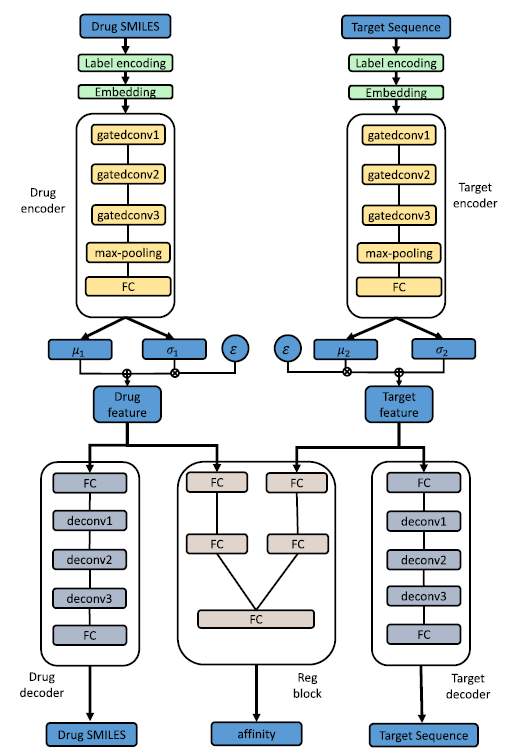
\includegraphics[width=0.94\linewidth]{presentation-figs/coVAE-block-diagram.png}
    \end{column}

    \begin{column}{0.61\textwidth}
      \begin{block}{مسیر بالا به پایین}
        \footnotesize
        \begin{enumerate}\itemsep0.3ex
          \item دو رمزگذار موازی --- \e{gatedconv}$\times$\e{3} + \e{max-pool} + \e{FC}
          \item فضای نهان --- \lr{$\mu$}، \lr{$\sigma$}، \lr{$\varepsilon$} و بازپارامتری‌سازی
        \end{enumerate}
      \end{block}

      \vspace{0.8mm}
      \begin{exampleblock}{سه سر خروجی از \e{drug} / \e{target feature}}
        \footnotesize
        \begin{itemize}\itemsep0.25ex
          \item \e{Drug decoder} --- بازسازی \e{SMILES}
          \item \E{Reg block} --- پیش‌بینی \key{\e{affinity}}
          \item \e{Target decoder} --- بازسازی توالی هدف
        \end{itemize}
      \end{exampleblock}

      \vspace{1.5mm}
      {\footnotesize\color{nxgray}
       همان دو فضای نهان هم‌زمان \key{بازسازی} و \key{رگرسیون} را تغذیه
       می‌کنند؛ همین اشتراک نقش \e{co-regularization} را بازی می‌کند.}
    \end{column}
  \end{columns}
  \note{تفاوت ساختاری مهم با \e{DCGAN-DTA}: آنجا پیش‌آموزش و رگرسیون دو مرحله‌ی جدا بودند، اینجا بازسازی و رگرسیون هم‌زمان و از یک فضای نهان مشترک آموزش می‌بینند. اگر پرسیده شد \e{co-regularization} دقیقاً چیست: یک جمله‌ی اضافه در تابع هزینه، علاوه بر دو جمله‌ی بازسازی و دو جمله‌ی \e{KL}، که فضاهای نهان دارو و هدف را طوری شکل می‌دهد که از رویشان بتوان \e{affinity} را بازیابی کرد.}
\end{frame}

%======================================================================
\section{مقایسه و خلأ پژوهشی}
%======================================================================

%--------------------------------------------------------------- 19 --
\begin{frame}{مقایسه‌ی دو رویکرد}
  \framesubtitle{\e{DCGAN-DTA} در برابر \e{Co-VAE}}
  \vspace{2mm}
  \centering
  {\footnotesize
  \rowcolors{2}{nxlight}{white}
  \begin{tabular}{p{0.22\textwidth} p{0.30\textwidth} p{0.30\textwidth}}
    \rowcolor{nxdark}
    \thd{ویژگی} & \thd{\e{DCGAN-DTA}} & \thd{\e{Co-VAE}} \\
    نوع مدل            & \e{GAN}                          & \e{VAE} \\
    ایده‌ی اصلی        & \e{Adversarial learning}         & \e{Variational learning} \\
    اجزا               & \e{Generator} + \e{Discriminator}& \e{Encoder} + \e{Decoder} \\
    فضای نهان          & تخاصمی / مولد                    & احتمالاتی \\
    نمایش دارو         & \e{SMILES}                       & \e{SMILES} \\
    نمایش هدف          & \e{Protein sequence}             & \e{Protein sequence} \\
    خروجی              & \e{Prediction}                   & \e{Prediction} + \e{co-regularization} \\
    هدف جانبی          & یادگیری نمایش                    & تولید + یادگیری نمایش \\
  \end{tabular}}

  \vspace{4mm}
  \begin{alertblock}{جمله‌ی کلیدی}
    \centering
    تفاوت اصلی این دو مقاله فقط در \e{architecture} نیست؛ آن‌ها
    \key{دو دیدگاه متفاوت} نسبت به یادگیری نمایش دارند.
  \end{alertblock}
  \note{این جدول را سطر به سطر نخوان. فقط سه سطر اول را بگو و مستقیم برو سراغ جمله‌ی پایین اسلاید، چون همان جمله ورودی بخش نوآوری است.}
\end{frame}

%--------------------------------------------------------------- 20 --
\begin{frame}{خلأ پژوهشی}
  \framesubtitle{\e{Research Gap}}
  \vspace{3mm}
  \begin{columns}[T]
    \begin{column}{0.47\textwidth}
      \begin{block}{\e{DCGAN-DTA}}
        \small تمرکز بر یادگیری نمایش مبتنی بر \e{GAN} برای \e{DTA}.
      \end{block}
      \vspace{2mm}
      \begin{exampleblock}{\e{Co-VAE}}
        \small تمرکز بر نمایش وردشی به‌همراه \e{co-regularization} برای \e{DTA}.
      \end{exampleblock}
    \end{column}

    \begin{column}{0.49\textwidth}
      \centering
      \vspace{1mm}
      \begin{tikzpicture}[font=\footnotesize,node distance=5mm]
        \node[nxn,minimum width=24mm,fill=nxblue!18,draw=nxblue!80] (a) {\e{DCGAN-DTA}};
        \node[nxn,minimum width=24mm,right=10mm of a,fill=nxteal!18,draw=nxteal!80] (b) {\e{Co-VAE}};
        \node[ghost,minimum width=40mm,below=10mm of $(a)!0.5!(b)$,draw=nxred!70,dashed,text=nxred]
          (g) {\fa{پروتکل آزمایشی مشترک؟}};
        \draw[arrd,draw=nxred!70] (a) -- (g);
        \draw[arrd,draw=nxred!70] (b) -- (g);
      \end{tikzpicture}
    \end{column}
  \end{columns}

  \vspace{4mm}
  \begin{alertblock}{خلأ}
    \centering
    مقایسه‌ی \key{مستقیم و کنترل‌شده}ی این دو پارادایم تحت یک
    \e{experimental protocol} مشترک، مسئله‌ای است که در این پایان‌نامه بررسی می‌شود.
  \end{alertblock}
  \note{اینجا محتاط باش و ادعای بزرگ نکن. نگو «هیچ‌کس این کار را نکرده»؛ بگو «تا جایی که بررسی کرده‌ام، مقایسه‌ی کنترل‌شده‌ی این دو خانواده تحت یک پروتکل یکسان کمتر انجام شده است». این جمله قابل دفاع‌تر است.}
\end{frame}

%======================================================================
\section{نوآوری پیشنهادی}
%======================================================================

%--------------------------------------------------------------- 21 --
\begin{frame}{نوآوری‌های پیشنهادی}
  \framesubtitle{چهار محور اصلی پایان‌نامه}
  \vspace{3mm}
  \begin{columns}[T]
    \begin{column}{0.48\textwidth}
      \small
      \begin{block}{۱. مقایسه‌ی دو پارادایم مولد}
        \e{Adversarial learning} در برابر \e{Variational learning}
        برای مسئله‌ی \e{DTA}.
      \end{block}

      \vspace{1mm}
      \begin{block}{۲. پروتکل آزمایشی یکسان}
        مجموعه‌داده، \e{preprocessing}، نمایش‌ها، \e{split}، معیارها و
        \e{seed}های کنترل‌شده --- تا تفاوت عملکرد واقعاً به
        \e{architecture} نسبت داده شود.
      \end{block}
    \end{column}

    \begin{column}{0.48\textwidth}
      \small
      \begin{block}{۳. بررسی \e{generalization}}
        مقایسه در دو شرایط \e{warm-start} و \e{cold-start}؛ عملکرد روی
        \e{random split} لزوماً توان پیش‌بینی برای داروها و هدف‌های
        واقعاً جدید را نشان نمی‌دهد.
      \end{block}

      \vspace{1mm}
      \begin{block}{۴. تحلیل فراتر از دقت}
        علاوه بر \e{performance}: \e{generalization}،
        \e{training stability}، \e{computational cost} و
        \e{data efficiency}.
      \end{block}
    \end{column}
  \end{columns}

  \vspace{3mm}
  \centering
  {\footnotesize\color{nxgray}
   \e{DCGAN-DTA} نیز همین مسئله را با \e{warm-start} و \e{cold-start} فیزیکوشیمیایی مورد توجه قرار داده است.}
  \note{مهم‌ترین اسلاید دفاع از نوآوری. اگر استاد گفت «این فقط مقایسه است، نوآوری نیست»، پاسخ آماده داشته باش: نوآوری در طراحی پروتکل کنترل‌شده و در تحلیل چندبعدی (نه صرفاً عدد دقت) است، و خروجی آن یک راهنمای انتخاب مدل برای این حوزه است.}
\end{frame}

%--------------------------------------------------------------- 22 --
\begin{frame}{سؤال اصلی پژوهش}
  \framesubtitle{پرسش اصلی و پرسش‌های فرعی}
  \vspace{2mm}
  \begin{alertblock}{پرسش اصلی}
    \centering
    آیا نوع روش یادگیری مولد --- \key{تخاصمی} یا \key{وردشی} --- می‌تواند بر
    کیفیت یادگیری نمایش و عملکرد پیش‌بینی قدرت اتصال در مسئله‌ی \e{DTA}
    تأثیر معناداری داشته باشد؟
  \end{alertblock}

  \vspace{1.5mm}
  \begin{block}{پرسش‌های فرعی}
    \footnotesize
    \begin{enumerate}\itemsep0.35ex
      \item کدام روش در \e{warm-start} عملکرد بهتری دارد؟
      \item کدام روش در \e{cold-start} بهتر \e{generalize} می‌کند؟
      \item حساسیت هر مدل نسبت به حجم داده چقدر است؟
      \item کدام مدل از نظر \e{computational cost} مناسب‌تر است؟
      \item آیا برتری مشاهده‌شده ناشی از \e{architecture} است یا از
            \e{dataset} / \e{split} / \e{preprocessing}؟
    \end{enumerate}
  \end{block}
  \note{ارائه باید با همین اسلاید به اوج برسد. پرسش پنجم مهم‌ترین است و نشان می‌دهد به اعتبار درونی آزمایش فکر کرده‌ای؛ روی همان یک مکث کوتاه کن.}
\end{frame}

%--------------------------------------------------------------- 23 --
\begin{frame}{روایت کلی ارائه}
  \framesubtitle{جمع‌بندی بصری مسیر ارائه}
  \vspace{3mm}
  \centering
  % سه سطر: صورت‌مسئله، مسیر روش‌ها، و جمع‌بندی به نوآوری
  \begin{tikzpicture}[x=1mm,y=1mm,font=\scriptsize]
    % --- row 1: the problem ---
    \node[ghost,minimum width=20mm] (dti) at (14,24) {\e{DTI}};
    \node[ghost,minimum width=20mm] (dta) at (44,24) {\e{DTA}};
    \node[nxn,minimum width=30mm]   (aff) at (84,24) {\e{Binding affinity}};
    \draw[arr] (dti)--(dta); \draw[arr] (dta)--(aff);
    % برچسب‌ها بالای سطر اول تا مسیر اتصال به سطر دوم آزاد بماند
    \node[lbl,text width=22mm,align=center] at (14,32) {\fa{هست یا نیست؟}};
    \node[lbl,text width=22mm,align=center] at (44,32) {\fa{چقدر قوی؟}};
    \node[lbl,text width=30mm,align=center] at (84,32) {\e{Kd} / \e{Ki} / \e{IC50}};

    % --- row 2: how the field got here ---
    \node[ghost,minimum width=18mm] (cls) at (11,4)  {\fa{کلاسیک}};
    \node[ghost,minimum width=13mm] (mlx) at (33,4)  {\e{ML}};
    \node[model,minimum width=13mm] (dlx) at (53,4)  {\e{DL}};
    \node[model,minimum width=32mm] (rep) at (87,4)  {\e{Representation learning}};
    \node[res,minimum width=18mm]   (gen) at (117,4) {\fa{مدل‌های مولد}};
    \draw[arr] (cls)--(mlx); \draw[arr] (mlx)--(dlx);
    \draw[arr] (dlx)--(rep); \draw[arr] (rep)--(gen);
    \draw[arr] (aff.south) -- ++(0,-6) -| (cls.north);

    % --- row 3: the two papers, the comparison, the contribution ---
    \node[nxn,minimum width=24mm,fill=nxblue!18,draw=nxblue!80] (g1) at (14,-16) {\e{DCGAN-DTA}};
    \node[nxn,minimum width=18mm,fill=nxteal!18,draw=nxteal!80] (g2) at (42,-16) {\e{Co-VAE}};
    \node[nxn,minimum width=30mm,draw=nxred!70,fill=nxred!8]    (cmp) at (80,-16) {\fa{مقایسه‌ی کنترل‌شده}};
    \node[res,minimum width=26mm,fill=nxaccent!30,draw=nxaccent] (nov) at (115,-16) {\fa{نوآوری پایان‌نامه}};
    \draw[arr] (g1)--(g2);
    \draw[arr] (g2)--(cmp);
    \draw[arr] (cmp)--(nov);
    \draw[arr] (gen.south) -- ++(0,-5) -| (g1.north);
  \end{tikzpicture}
  \note{این اسلاید جمع‌بندی بصری است. می‌توانی آن را ۱۵ ثانیه‌ای رد کنی یا اگر جلسه طولانی شد مستقیم از اسلاید ۲۲ به اسلاید پرسش‌ها بروی.}
\end{frame}

%--------------------------------------------------------------- 24 --
\begin{frame}{مراجع اصلی}
  \framesubtitle{منابع کلیدی این ارائه}
  \vspace{4mm}
  \small
  % هر مرجع یک بازه‌ی کامل چپ‌به‌راست است تا ترتیب اجزای استناد به‌هم نریزد
  \vspace{-2mm}
  \begin{enumerate}\footnotesize\itemsep0.35ex
    \item \lr{Wang et al., \textit{A unified survey on drug--target interaction
          and binding affinity prediction}, Biotechnology Advances, 2026.}
    \item \lr{Pahikkala et al., \textit{Toward more realistic drug--target
          interaction predictions} (KronRLS), Brief.\ Bioinform., 2015.}
    \item \lr{He et al., \textit{SimBoost: a read-across approach using gradient
          boosting machines}, J.\ Cheminformatics, 2017.}
    \item \lr{Öztürk et al., \textit{DeepDTA: deep drug--target binding affinity
          prediction}, Bioinformatics, 2018.}
    \item \lr{Öztürk et al., \textit{WideDTA: prediction of drug--target binding
          affinity}, arXiv, 2019.}
    \item \lr{Nguyen et al., \textit{GraphDTA: predicting drug--target binding
          affinity with graph neural networks}, Bioinformatics, 2021.}
    \item \lr{Li et al., \textit{Co-VAE: Drug--Target Binding Affinity Prediction
          by Co-Regularized Variational Autoencoders}, IEEE TPAMI, 2022.}
    \item \lr{Kalemati et al., \textit{DCGAN-DTA: Predicting drug--target binding
          affinity with deep convolutional GANs}, BMC Genomics, 2024.}
  \end{enumerate}

  \vspace{4mm}
  {\footnotesize\color{nxgray}
   فهرست کامل مراجع در متن پایان‌نامه ارائه شده است.}
  \note{این اسلاید فقط برای مستند بودن است؛ روی آن توقف نکن مگر استاد سؤال کند.}
\end{frame}

%--------------------------------------------------------------- 25 --
\begin{frame}[plain,noframenumbering]
  \vfill
  \begin{center}
    {\lr{\textcolor{nxaccent}{\rule{28mm}{1.6pt}}}}\\[6mm]
    {\Large\bfseries\color{nxdark} با تشکر از توجه شما}\\[5mm]
    {\large\color{nxgray} پرسش‌ها و پیشنهادها}\\[8mm]
    {\small محسن کاشفی کیا \quad$\cdot$\quad استاد راهنما: دکتر سایه میرزایی}
  \end{center}
  \vfill
  \note{آماده باش برای این سه سؤال: (۱) چرا همین دو مقاله را انتخاب کردی؟ (۲) داده و منابع محاسباتی را چطور تأمین می‌کنی؟ (۳) اگر نتیجه این شد که تفاوت معنادار نیست، دستاورد پایان‌نامه چیست؟ برای سؤال سوم پاسخ بده: نتیجه‌ی منفی هم یافته است، چون نشان می‌دهد تفاوت گزارش‌شده در مقالات ناشی از پروتکل بوده نه معماری.}
\end{frame}

\end{document}
"
%======================================================================
\documentclass[11pt,aspectratio=169,xcolor=table]{beamer}

\usetheme{default}
\usecolortheme{default}
\setbeamertemplate{navigation symbols}{}

\usepackage{amsmath,amssymb}
\usepackage{xcolor}
\usepackage{tikz}
\usetikzlibrary{arrows.meta,positioning,shapes.geometric,fit,backgrounds,calc,decorations.pathreplacing}
\usepackage{array}

%------------------------------- palette ------------------------------
\definecolor{nxdark}{HTML}{16334F}
\definecolor{nxblue}{HTML}{2F6FA8}
\definecolor{nxteal}{HTML}{2A7F6F}
\definecolor{nxaccent}{HTML}{D9743B}
\definecolor{nxred}{HTML}{B5453A}
\definecolor{nxgray}{HTML}{6B7785}
\definecolor{nxlight}{HTML}{EDF2F7}

%------------------------------- fonts --------------------------------
\usepackage{xepersian}
\settextfont[Scale=1.0]{XB Zar}
\setdigitfont[Scale=1.0]{XB Zar}
\setlatintextfont[Scale=0.92]{Cambria}

% سازگاری: وصله‌ی bidi برای jadval به ماکرویی ارجاع می‌دهد که از نسخه‌های
% جدید array.sty حذف شده است.
\providecommand\UseMathForPositioningText{}

%------------------------------ beamer look ---------------------------
\setbeamercolor{structure}{fg=nxdark}
\setbeamercolor{frametitle}{fg=white,bg=nxdark}
\setbeamercolor{framesubtitle}{fg=nxgray}
\setbeamercolor{footline}{fg=nxgray}
\setbeamercolor{normal text}{fg=nxdark!95}
\setbeamercolor{itemize item}{fg=nxaccent}
\setbeamercolor{itemize subitem}{fg=nxblue}
\setbeamercolor{block title}{fg=white,bg=nxblue}
\setbeamercolor{block body}{fg=nxdark,bg=nxblue!8}
\setbeamercolor{block title alerted}{fg=white,bg=nxaccent}
\setbeamercolor{block body alerted}{fg=nxdark,bg=nxaccent!10}
\setbeamercolor{block title example}{fg=white,bg=nxteal}
\setbeamercolor{block body example}{fg=nxdark,bg=nxteal!8}

\setbeamerfont{frametitle}{size=\large,series=\bfseries}
\setbeamerfont{framesubtitle}{size=\small}
\setbeamerfont{footline}{size=\scriptsize}
\setbeamerfont{block title}{size=\small,series=\bfseries}
\setbeamerfont{block body}{size=\small}

\setbeamertemplate{itemize item}{\raisebox{0.15ex}{\tiny$\blacktriangleleft$}}
\setbeamertemplate{itemize subitem}{\raisebox{0.15ex}{\tiny$\blacktriangleleft$}}
% قالب rounded بیمر با bidi به‌هم می‌ریزد؛ قالب ساده پایدار است.
\setbeamertemplate{blocks}[default]

% ---- frame title: full-width bar + accent rule ----
\definecolor{nxsub}{HTML}{A9BDD1}
\setbeamercolor{nxrule}{bg=nxaccent,fg=nxaccent}
\setbeamercolor{framesubtitle}{fg=nxsub,bg=nxdark}

% نکته‌ی مهم درباره‌ی bidi: در قالب‌های بیمر، فقط نخستین beamercolorbox رسم
% می‌شود و \rule داخل متن راست‌به‌چپ رنگ خود را از دست می‌دهد (سیاه می‌شود).
% بنابراین همه‌ی تزئینات (خط نارنجی سربرگ و نوار پیشرفت پاورقی) با tikz در
% قالب background canvas کشیده می‌شوند و سربرگ همیشه دو سطری است تا ارتفاع
% آن ثابت بماند.
\makeatletter
\setbeamertemplate{frametitle}{%
  \begin{beamercolorbox}[wd=\paperwidth,leftskip=1em,rightskip=1em]{frametitle}%
    \vspace{1.1ex}%
    {\usebeamerfont{frametitle}\insertframetitle}\\[0.1ex]%
    % هر اسلاید باید \framesubtitle داشته باشد تا ارتفاع سربرگ ثابت بماند و
    % خط نارنجیِ کشیده‌شده در background canvas دقیقاً زیر نوار بنشیند.
    {\usebeamerfont{framesubtitle}\usebeamercolor[fg]{framesubtitle}%
     \insertframesubtitle}%
    \vspace{1.0ex}%
  \end{beamercolorbox}%
}
\makeatother

% ---- footer: section name + frame number (chrome drawn in background) ----
\setbeamertemplate{footline}{%
  \begin{beamercolorbox}[wd=\paperwidth,ht=2.4ex,dp=1.4ex,leftskip=1em,rightskip=1em]{footline}%
    \usebeamerfont{footline}%
    \insertsectionhead\hfill\insertframenumber\,/\,\inserttotalframenumber%
  \end{beamercolorbox}%
}

% ---- all decorative chrome, drawn with tikz so bidi cannot swallow it ----
\newlength{\nxprogw}
\newlength{\nxhdrh}
\setlength{\nxhdrh}{37.2pt}    % ارتفاع نوار سربرگ (دو سطری، ثابت)
\makeatletter
\setbeamertemplate{background canvas}{%
  \setlength{\nxprogw}{\dimexpr\paperwidth/\inserttotalframenumber*\insertframenumber\relax}%
  \begin{tikzpicture}[overlay,remember picture]
    \fill[white] (current page.south west) rectangle (current page.north east);
    \ifbeamer@plainframe\else
      \fill[nxaccent] (current page.north west) ++(0,-\nxhdrh)
                      rectangle ++(\paperwidth,-1.2pt);
    \fi
    \fill[nxdark!12] (current page.south west) rectangle ++(\paperwidth,1pt);
    \fill[nxaccent]  (current page.south east) ++(-\nxprogw,0)
                     rectangle ++(\nxprogw,1pt);
  \end{tikzpicture}%
}
\makeatother

% ---- notes ----
\ifdefined\notesmode
  \setbeameroption{show only notes}
\else
  \setbeameroption{hide notes}
\fi
\setbeamerfont{note page}{size=\small}

%------------------------------ tikz styles ---------------------------
\tikzset{
  nxn/.style   ={draw=nxdark!55, rounded corners=2.5pt, fill=white,
                 inner xsep=6pt, inner ysep=4pt, minimum height=8mm,
                 font=\small, align=center},
  drug/.style  ={nxn, fill=nxblue!12,   draw=nxblue!75},
  targ/.style  ={nxn, fill=nxteal!12,   draw=nxteal!75},
  model/.style ={nxn, fill=nxdark!10,   draw=nxdark!60},
  res/.style   ={nxn, fill=nxaccent!16, draw=nxaccent!85},
  ghost/.style ={nxn, fill=nxlight,     draw=nxdark!25, text=nxgray},
  lbl/.style   ={font=\scriptsize, text=nxgray, inner sep=2pt},
  arr/.style   ={-{Stealth[length=2.1mm,width=1.6mm]}, draw=nxdark!70, thick},
  arrd/.style  ={arr, dashed},
  flat/.style  ={draw=none, fill=none, font=\small, align=center},
}

%-------------------------- small helper macros -----------------------
\newcommand{\E}[1]{\lr{\textbf{#1}}}
\newcommand{\e}[1]{\lr{#1}}
% متن فارسی داخل گره‌های tikz به صورت پاراگراف چپ‌به‌راست چیده می‌شود و ترتیب
% واژه‌ها برعکس می‌شود؛ \fa کل متن گره را در یک بازه‌ی راست‌به‌چپ قرار می‌دهد.
% توجه: داخل \fa نباید \\ بیاید — هر سطر را جداگانه باید پیچید.
\newcommand{\fa}[1]{\RLE{#1}}
% ریاضیِ نمایشی: \[...\] در ستون راست‌به‌چپ سرریز می‌کند و دیده نمی‌شود؛
% همچنین \lr باعث می‌شود ارقام داخل فرمول لاتین بمانند نه فارسی.
\newcommand{\disp}[1]{\begin{center}\lr{$\displaystyle #1$}\end{center}}
\newcommand{\key}[1]{\textcolor{nxaccent}{\textbf{#1}}}
\newcommand{\thd}[1]{\textcolor{white}{\textbf{#1}}}

% section divider
\AtBeginSection[]{%
  \begin{frame}[plain,noframenumbering]
    \vfill
    \begin{center}
      {\lr{\textcolor{nxaccent}{\rule{22mm}{1.6pt}}}}\\[4mm]
      {\usebeamerfont{frametitle}\Large\color{nxdark}\insertsectionhead}\\[3mm]
      {\lr{\textcolor{nxdark!20}{\rule{60mm}{0.7pt}}}}
    \end{center}
    \vfill
  \end{frame}
}

\begin{document}

%======================================================================
% TITLE
%======================================================================
\begin{frame}[plain,noframenumbering]
  \vspace{-3mm}
  \hbox to\textwidth{%
    
\includegraphics[height=11mm]{First-Pages/TehUni.png}\hfill
    
\includegraphics[height=11mm]{First-Pages/Eng.png}}

  \vspace{-6mm}
  \begin{center}
    {\footnotesize دانشگاه تهران — پردیس دانشکده‌های فنی}\\[0.4mm]
    {\footnotesize دانشکده علوم مهندسی — گروه الگوریتم‌ها و محاسبات}

    \vspace{3mm}
    {\lr{\textcolor{nxaccent}{\rule{30mm}{1.2pt}}}}

    \vspace{2.5mm}
    {\large\bfseries\color{nxdark} پیش‌بینی قدرت اتصال دارو--هدف\\[1mm]
     با مدل‌های مولد}\\[2mm]
    {\small\color{nxgray} مقایسه‌ی کنترل‌شده‌ی یادگیری تخاصمی و یادگیری وردشی}\\[0.6mm]
    {\scriptsize\color{nxgray}\e{Adversarial vs.\ Variational Representation Learning for Drug--Target Affinity}}

    \vspace{3mm}
    {\lr{\textcolor{nxdark!20}{\rule{70mm}{0.5pt}}}}\\[2mm]

    {\footnotesize ارائه‌دهنده: \textbf{محسن کاشفی کیا}}\\[0.8mm]
    {\footnotesize استاد راهنما: \textbf{دکتر سایه میرزایی}}\\[2mm]
    {\scriptsize\color{nxgray} گزارش پیشرفت پایان‌نامه کارشناسی ارشد \quad$\cdot$\quad شهریور ۱۴۰۵}
  \end{center}
  \note{سلام و تشکر از استاد. در یک جمله بگو: «هدف این جلسه این است که مسیر رسیدن از صورت‌مسئله تا نوآوری پیشنهادی پایان‌نامه را مرور کنیم.» زمان پیشنهادی کل ارائه: ۲۰ تا ۲۵ دقیقه.}
\end{frame}

%======================================================================
% OUTLINE
%======================================================================
\begin{frame}{فهرست مطالب}
  \framesubtitle{مسیر ارائه در یک نگاه}
  \vspace{3mm}
  \begin{columns}[T]
    \begin{column}{0.52\textwidth}
      \small
      \begin{enumerate}
        \item تعریف مسئله: از \e{DTI} تا \e{DTA}
        \item معیارهای کمی قدرت اتصال
        \item درخت تکاملی روش‌ها: از \e{KronRLS} تا مدل‌های بنیادی
        \item جایگاه پایان‌نامه در این درخت
        \item مقاله‌ی اول: \e{DCGAN-DTA} --- شاخه‌ی \e{GAN}
        \item مقاله‌ی دوم: \e{Co-VAE} --- شاخه‌ی \e{VAE}
        \item خلأ پژوهشی و نوآوری پیشنهادی
      \end{enumerate}
    \end{column}
    \begin{column}{0.44\textwidth}
      \begin{tikzpicture}[node distance=4.5mm,every node/.style={font=\scriptsize}]
        \node[ghost,minimum width=32mm] (a) {\fa{\e{DTI} — آیا برهم‌کنش هست؟}};
        \node[ghost,minimum width=32mm,below=of a] (b) {\fa{\e{DTA} — چقدر قوی است؟}};
        \node[model,minimum width=32mm,below=of b] (c) {\fa{مسیر پژوهشی تا مدل‌های مولد}};
        \node[res,minimum width=32mm,below=of c] (d) {\fa{نوآوری پیشنهادی}};
        \draw[arr] (a)--(b); \draw[arr] (b)--(c); \draw[arr] (c)--(d);
      \end{tikzpicture}
    \end{column}
  \end{columns}
  \note{این اسلاید نقشه‌ی راه است. یک جمله بگو: «ارائه از صورت‌مسئله شروع می‌شود، به دو مقاله‌ی مرجع می‌رسد و با سؤال پژوهشی پایان‌نامه تمام می‌شود.» روی آن معطل نشو.}
\end{frame}

%======================================================================
\section{تعریف مسئله}
%======================================================================

%---------------------------------------------------------------- 1 --
\begin{frame}{برهم‌کنش دارو--هدف چیست؟}
  \framesubtitle{\e{Drug--Target Interaction (DTI)}}
  \vspace{2mm}
  \begin{columns}[T]
    \begin{column}{0.46\textwidth}
      \small
      در فرآیند \e{drug discovery}، یکی از مسائل پایه شناسایی ارتباط میان
      \key{دارو} و \key{پروتئین هدف} است.

      \vspace{2mm}
      \begin{block}{پرسش \e{DTI}}
        آیا یک دارو می‌تواند با یک پروتئین هدف برهم‌کنش داشته باشد یا خیر؟
      \end{block}

      \vspace{1mm}
      {\footnotesize\color{nxgray}
       خروجی مسئله \key{دودویی} است: بله / خیر.}
    \end{column}
    \begin{column}{0.50\textwidth}
      \centering
      \begin{tikzpicture}[node distance=7mm]
        \node[drug]                       (d) {\e{Drug D}};
        \node[targ, right=14mm of d]      (t) {\e{Target T}};
        \node[model, below=9mm of $(d)!0.5!(t)$, minimum width=34mm] (i) {\e{Interaction?}};
        \node[res,  below left=9mm and 1mm of i]  (y) {\e{Yes}};
        \node[ghost,below right=9mm and 1mm of i] (n) {\e{No}};
        \draw[arr] (d) -- (i);
        \draw[arr] (t) -- (i);
        \draw[arr] (i) -- (y);
        \draw[arr] (i) -- (n);
      \end{tikzpicture}
    \end{column}
  \end{columns}
  \note{\e{DTI} را به عنوان مسئله‌ی پایه معرفی کن: «اگر بخواهیم فضای جستجوی \e{drug discovery} را کوچک کنیم، اولین سؤال این است که از میان تعداد زیادی دارو و پروتئین، کدام جفت‌ها احتمالاً با هم برهم‌کنش دارند.» مقاله‌ی \e{Co-VAE} هم مقدمه‌اش را از همین نقطه شروع می‌کند.}
\end{frame}

%---------------------------------------------------------------- 2 --
\begin{frame}{از تشخیص برهم‌کنش به اندازه‌گیری قدرت آن}
  \framesubtitle{چرا پاسخ بله/خیر کافی نیست؟}
  \vspace{1mm}
  \centering
  \begin{tikzpicture}[x=1mm,y=1mm,font=\footnotesize]
    % --- inputs ---
    \node[drug] (d1) at (0,7)   {\e{Drug A}};
    \node[drug] (d2) at (0,-7)  {\e{Drug B}};
    \node[targ] (tx) at (28,0)  {\e{Target X}};
    \draw[arr] (d1) -- (tx);
    \draw[arr] (d2) -- (tx);

    % --- DTI column ---
    \node[lbl,text=nxdark,font=\scriptsize\bfseries] at (60,17) {\fa{دیدِ \e{DTI}}};
    \node[res,minimum width=26mm]   (y1) at (60,7)  {\e{Yes}};
    \node[res,minimum width=26mm]   (y2) at (60,-7) {\e{Yes}};
    \draw[arr] (tx) -- (y1);
    \draw[arr] (tx) -- (y2);
    \node[lbl,text width=32mm,align=center] at (60,-17) {\fa{هر دو یکسان دیده می‌شوند}};

    % --- divider ---
    \draw[nxdark!20,thick] (80,20) -- (80,-20);

    % --- DTA column ---
    \node[lbl,text=nxdark,font=\scriptsize\bfseries] at (104,17) {\fa{دیدِ \e{DTA}}};
    \node[nxn,minimum width=28mm,fill=nxred!18,draw=nxred!80] (s1) at (104,7)  {\e{Strong binding}};
    \node[ghost,minimum width=28mm]                           (s2) at (104,-7) {\e{Weak binding}};
    \draw[arr,draw=nxdark!35] (y1) -- (s1);
    \draw[arr,draw=nxdark!35] (y2) -- (s2);
    \node[lbl,text width=34mm,align=center] at (104,-17) {\fa{دو دارو از هم تفکیک می‌شوند}};
  \end{tikzpicture}

  \vspace{2mm}
  \begin{alertblock}{پرسش دقیق‌تر}
    \centering قدرت اتصال دارو به هدف \key{چقدر} است؟ \quad$\Rightarrow$\quad مسئله‌ی \E{Drug--Target Binding Affinity (DTA)}
  \end{alertblock}
  \note{نکته‌ی کلیدی: دو دارو می‌توانند هر دو با یک \e{target} برهم‌کنش داشته باشند، ولی یکی اتصال بسیار قوی و دیگری اتصال ضعیف. \e{DTI} این تفاوت را نمی‌بیند. اینجا گذار از مسئله‌ی دسته‌بندی به مسئله‌ی رگرسیون اتفاق می‌افتد.}
\end{frame}

%---------------------------------------------------------------- 3 --
\begin{frame}{چرا \e{DTA}؟}
  \framesubtitle{اطلاعات کمی در برابر اطلاعات دودویی}
  \vspace{2mm}
  \centering
  {\small
  \rowcolors{2}{nxlight}{white}
  \begin{tabular}{p{0.34\textwidth} p{0.34\textwidth}}
    \rowcolor{nxdark}
    \thd{\e{DTI}} & \thd{\e{DTA}} \\
    آیا برهم‌کنش وجود دارد؟ & برهم‌کنش چقدر قوی است؟ \\
    خروجی دودویی (\e{binary})   & خروجی پیوسته (\e{continuous}) \\
    بله / خیر                & مقدار عددی \e{affinity} \\
    مناسب غربالگری اولیه     & مناسب رتبه‌بندی و اولویت‌دهی \\
  \end{tabular}}

  \vspace{4mm}
  \begin{columns}[c]
    \begin{column}{0.55\textwidth}
      \begin{exampleblock}{جمله‌ی کلیدی}
        \e{DTA} علاوه بر \key{وجود} برهم‌کنش، \key{شدت} آن را نیز مشخص می‌کند و
        بنابراین اطلاعات غنی‌تری در اختیار می‌گذارد.
      \end{exampleblock}
    \end{column}
    \begin{column}{0.42\textwidth}
      {\footnotesize\color{nxgray}
       \textbf{دقت در بیان:} نگوییم «\e{DTA} همیشه بهتر از \e{DTI} است»؛
       این‌ها دو صورت‌بندی متفاوت از مسئله‌اند. بگوییم برای \emph{هدف این پژوهش}،
       اطلاعات کمی \e{affinity} ارزشمندتر است.}
    \end{column}
  \end{columns}
  \note{حتماً تأکید کن که \e{DTA} و \e{DTI} دو \e{formulation} متفاوت‌اند، نه اینکه یکی مطلقاً بهتر از دیگری باشد. این جمله از نظر علمی قابل دفاع‌تر است و معمولاً همین‌جا سؤال پرسیده می‌شود. \e{Co-VAE} هم پیش‌بینی \e{affinity} را چالش‌برانگیزتر از تشخیص \e{interaction} می‌داند.}
\end{frame}

%---------------------------------------------------------------- 4 --
\begin{frame}{قدرت اتصال چگونه اندازه‌گیری می‌شود؟}
  \framesubtitle{نقشه‌ی معیارهای متداول}
  \vspace{4mm}
  \centering
  \begin{tikzpicture}[node distance=5mm]
    \node[model,minimum width=30mm] (root) {\fa{اندازه‌گیری \e{Affinity}}};

    \node[targ,minimum width=44mm,below right=12mm and 2mm of root] (ba) {\e{Binding affinity}\\[-1mm] \fa{{\scriptsize قدرت اتصال ترمودینامیکی}}};
    \node[res, minimum width=40mm,below left=12mm and 2mm of root]  (po) {\e{Potency / inhibition}\\[-1mm] \fa{{\scriptsize اثر عملکردی در آزمایش}}};

    \node[nxn,below left=10mm and -2mm of ba]  (kd) {\e{Kd} \ / \ \e{pKd}};
    \node[nxn,below right=10mm and -2mm of ba] (ki) {\e{Ki} \ / \ \e{pKi}};
    \node[nxn,below=10mm of po]                (ic) {\e{IC50}};

    \draw[arr] (root) -- (ba);
    \draw[arr] (root) -- (po);
    \draw[arr] (ba) -- (kd);
    \draw[arr] (ba) -- (ki);
    \draw[arr] (po) -- (ic);
  \end{tikzpicture}

  \vspace{3mm}
  {\footnotesize\color{nxgray}
   در اسلایدهای بعد هر معیار جداگانه تعریف می‌شود؛ تمایز ستون راست و چپ نکته‌ی اصلی این بخش است.}
  \note{این اسلاید «نقشه» است. فقط بگو چهار پنج اصطلاح داریم و مهم‌ترین نکته این است که \e{Kd} و \e{Ki} معیار \e{binding affinity} هستند ولی \e{IC50} معیار \e{potency} عملکردی است. جزئیات را در اسلایدهای بعد باز می‌کنی.}
\end{frame}

%---------------------------------------------------------------- 5 --
\begin{frame}{\e{Kd} و \e{pKd}}
  \framesubtitle{\e{Equilibrium Dissociation Constant}}
  \vspace{1mm}
  \begin{columns}[T]
    \begin{column}{0.50\textwidth}
      \small
      \begin{block}{تعریف مفهومی}
        \e{Kd} غلظتی از \e{ligand} است که در شرایط تعادل، تقریباً \key{نیمی} از
        \e{target}ها را در حالت \e{bound} قرار می‌دهد.
      \end{block}

      \vspace{-1mm}
      \disp{K_d \;=\; \frac{[D]\,[T]}{[DT]}}

      \vspace{-3mm}
      {\footnotesize
      \e{D}: داروی آزاد \quad $\cdot$ \quad \e{T}: هدف آزاد \quad $\cdot$ \quad \e{DT}: کمپلکس دارو--هدف}

      \vspace{2mm}
      \begin{alertblock}{مقیاس لگاریتمی}
        \vspace{-3mm}
        \disp{pK_d \;=\; -\log_{10}\!\big(K_d\,[M]\big)}
        \vspace{-3mm}
        \centering اگر \lr{$K_d = 10^{-9}\,M$} آنگاه \lr{$pK_d = 9$}
      \end{alertblock}
    \end{column}

    \begin{column}{0.46\textwidth}
      \centering
      \vspace{3mm}
      % مقیاس به‌صورت راست‌به‌چپ خوانده می‌شود: سمت راست = اتصال قوی
      \begin{tikzpicture}
        \shade[left color=nxlight,right color=nxred!55] (0,0) rectangle (6.4,0.55);
        \draw[nxdark!35] (0,0) rectangle (6.4,0.55);
        \node[lbl,below] at (5.8,0) {\fa{\e{Kd} کوچک}};
        \node[lbl,below] at (0.6,0) {\fa{\e{Kd} بزرگ}};
        \node[lbl,above,text=nxdark,font=\scriptsize\bfseries] at (5.4,0.55) {\fa{اتصال قوی}};
        \node[lbl,above,text=nxdark,font=\scriptsize\bfseries] at (1.0,0.55) {\fa{اتصال ضعیف}};

        \node[drug,minimum width=24mm,below=11mm of {(5.4,0)},font=\scriptsize] (a)
          {\e{Drug A}\\[-1mm]{\scriptsize\e{Kd = 1 nM}}};
        \node[ghost,minimum width=24mm,below=11mm of {(1.0,0)},font=\scriptsize] (b)
          {\e{Drug B}\\[-1mm]{\scriptsize\e{Kd = 100 nM}}};
      \end{tikzpicture}

      \vspace{6mm}
      {\small\color{nxdark}
       \lr{$K_d \downarrow$} \quad$\Longrightarrow$\quad \e{affinity} \lr{$\uparrow$} \quad$\Longrightarrow$\quad \lr{$pK_d \uparrow$}}
    \end{column}
  \end{columns}
  \note{نکته‌ای که معمولاً پرسیده می‌شود: چرا لگاریتم می‌گیریم؟ چون مقادیر \e{Kd} در بازه‌ای بسیار وسیع و بسیار کوچک (نانومولار تا میکرومولار) پخش‌اند و مقیاس لگاریتمی هم عددها را قابل‌مدیریت می‌کند و هم برای رگرسیون مناسب‌تر است. جهت را اشتباه نگو: \e{Kd} کمتر یعنی \e{affinity} بیشتر.}
\end{frame}

%---------------------------------------------------------------- 6 --
\begin{frame}{\e{Ki} و \e{pKi}}
  \framesubtitle{\e{Inhibition Constant}}
  \vspace{2mm}
  \begin{columns}[T]
    \begin{column}{0.50\textwidth}
      \small
      \begin{block}{تعریف}
        \e{Ki} معیاری برای بیان \e{affinity} یک \key{مهارکننده} (\e{inhibitor})
        نسبت به \e{target} یا آنزیم است.
      \end{block}

      \vspace{1mm}
      هرچه \e{Ki} کوچک‌تر باشد، \e{inhibitor} تمایل بیشتری به اتصال مؤثر
      به \e{target} دارد.

      \vspace{-1mm}
      \disp{pK_i \;=\; -\log_{10}\!\big(K_i\,[M]\big)}

      \vspace{-2mm}
      \centering
      {\small \lr{$K_i \downarrow$} \quad$\Longrightarrow$\quad \lr{$pK_i \uparrow$} \quad$\Longrightarrow$\quad \e{affinity} \lr{$\uparrow$}}
    \end{column}

    \begin{column}{0.46\textwidth}
      \vspace{2mm}
      \begin{alertblock}{\e{Ki} و \e{Kd} یکی نیستند}
        \small
        \begin{itemize}
          \item \E{Kd}: مستقیماً \e{equilibrium dissociation} را در یک سامانه‌ی اتصال بیان می‌کند.
          \item \E{Ki}: در زمینه‌ی \e{inhibition} و برای بیان \e{potency/affinity} مهارکننده به کار می‌رود.
        \end{itemize}
      \end{alertblock}

      \vspace{1mm}
      {\footnotesize\color{nxgray}
       هر دو در ادبیات \e{DTA} به عنوان برچسب \e{affinity} استفاده می‌شوند؛
       مجموعه‌داده‌های مختلف برچسب‌های متفاوتی دارند.}
    \end{column}
  \end{columns}
  \note{اگر استاد پرسید تفاوت \e{Ki} و \e{Kd} چیست، همین اسلاید جواب است. اضافه کن که در عمل، مجموعه‌داده‌ها فرق دارند: \e{Davis} بر پایه‌ی \e{Kd} است و \e{KIBA} یک امتیاز ترکیبی است؛ بنابراین مقایسه‌ی اعداد بین مجموعه‌داده‌ها مستقیماً معنادار نیست.}
\end{frame}

%---------------------------------------------------------------- 7 --
\begin{frame}{\e{IC50}}
  \framesubtitle{\e{Half Maximal Inhibitory Concentration}}
  \vspace{1mm}
  \begin{columns}[T]
    \begin{column}{0.44\textwidth}
      \small
      \vspace{2mm}
      \begin{block}{تعریف}
        غلظتی از \e{inhibitor} که باعث \key{۵۰٪ کاهش} فعالیت یک سامانه یا
        آنزیم می‌شود.
      \end{block}

      \vspace{2mm}
      \begin{alertblock}{نکته‌ی مهم علمی}
        \e{IC50} مستقیماً \key{معیار \e{binding affinity} نیست}؛
        یک معیار \e{functional inhibition / potency} است و به شرایط
        آزمایش (مثلاً غلظت \e{substrate}) وابسته است.
      \end{alertblock}
    \end{column}

    \begin{column}{0.52\textwidth}
      \centering
      \vspace{4mm}
      \begin{tikzpicture}[xscale=1.25,yscale=1.0]
        \draw[->,nxdark!55,thick] (-0.15,0) -- (5.4,0);
        \draw[->,nxdark!55,thick] (0,-0.15) -- (0,3.7);
        \node[lbl,below] at (2.7,-0.25) {\e{log [Inhibitor]}};
        \node[lbl,rotate=90,above] at (-0.45,1.8) {\e{\% Inhibition}};

        \draw[nxaccent,very thick] plot[domain=0.15:5.1,samples=90,smooth]
             (\x,{3.2/(1+exp(-2.0*(\x-2.6)))});

        \draw[dashed,nxblue!80] (2.6,0) -- (2.6,1.6) -- (0,1.6);
        \fill[nxblue] (2.6,1.6) circle (1.6pt);
        \node[lbl,text=nxblue,below] at (2.6,-0.02) {\e{IC50}};
        \node[lbl,text=nxblue,left]  at (-0.05,1.6) {\e{50\%}};
        \node[lbl,left] at (-0.05,3.2) {\e{100\%}};
      \end{tikzpicture}

      \vspace{2mm}
      {\footnotesize\color{nxgray}
       منحنی پاسخ به غلظت؛ \e{IC50} نقطه‌ی رسیدن به نیمه‌ی حداکثر مهار است.}
    \end{column}
  \end{columns}
  \note{این تمایز را حتماً بگو، چون از نظر علمی مهم است و نشان می‌دهد ادبیات را دقیق خوانده‌ای: \e{Kd} و \e{Ki} معیار اتصال‌اند، \e{IC50} معیار اثر عملکردی. ادبیات مقایسه‌ی ابزارهای \e{DTA} هم صراحتاً روی همین تأکید می‌کند.}
\end{frame}

%---------------------------------------------------------------- 8 --
\begin{frame}{جمع‌بندی معیارهای اتصال و مهار}
  \framesubtitle{کدام معیار چه چیزی را می‌سنجد؟}
  \vspace{3mm}
  \centering
  {\small
  \rowcolors{2}{nxlight}{white}
  \begin{tabular}{p{0.16\textwidth} p{0.34\textwidth} p{0.28\textwidth}}
    \rowcolor{nxdark}
    \thd{معیار} & \thd{مفهوم} & \thd{مقدار کمتر یعنی} \\
    \E{Kd}   & \e{Dissociation constant}        & \e{affinity} بیشتر \\
    \E{pKd}  & \e{−log\textsubscript{10}(K\textsubscript{d})} & \e{affinity} بیشتر \\
    \E{Ki}   & \e{Inhibition constant}          & \e{affinity} بیشتر \\
    \E{pKi}  & \e{−log\textsubscript{10}(K\textsubscript{i})} & \e{affinity} بیشتر \\
    \E{IC50} & غلظت لازم برای ۵۰٪ مهار          & \e{potency} بیشتر \\
  \end{tabular}}

  \vspace{5mm}
  \begin{exampleblock}{کاربرد در عمل}
    در بسیاری از \e{benchmark}های \e{DTA}، مقادیر \e{affinity} به شکل
    \key{لگاریتمی} مانند \e{pKd} یا \e{pKi} استفاده می‌شوند.
    برای نمونه \e{DCGAN-DTA} روی \e{BindingDB} مقادیر را به \e{pKd} تبدیل کرده
    و \e{PDBBind} نیز شامل مقادیر \e{log-transformed} از \e{Ki} و \e{Kd} است.
  \end{exampleblock}
  \note{این اسلاید پل به بخش بعد است. بگو: «پس برچسبی که مدل‌ها پیش‌بینی می‌کنند معمولاً یک عدد پیوسته در مقیاس لگاریتمی است؛ حالا ببینیم پژوهشگران برای پیش‌بینی این عدد چه مسیری را طی کرده‌اند.»}
\end{frame}

%======================================================================
\section{مسیر پژوهشی}
%======================================================================

%---------------------------------------------------------------- 9 --
\begin{frame}{درخت تکاملی روش‌های پیش‌بینی \e{DTA}}
  \framesubtitle{از ۲۰۱۵ تا ۲۰۲۶ --- بر پایه‌ی مرور \e{Wang et al.}, \e{Biotechnology Advances}, ۲۰۲۶}
  \vspace{1mm}
  \centering
  \begin{tikzpicture}[x=1mm,y=1mm,
      tn/.style={nxn,minimum height=6.6mm,inner xsep=3pt,inner ysep=1.5pt,
                 font=\tiny,align=center},
      bus/.style={draw=nxdark!65,thick},
      dn/.style={-{Stealth[length=1.8mm,width=1.4mm]},draw=nxdark!65,thick}]

    % ---- tier A: the historical spine --------------------------------
    \node[tn,ghost,minimum width=34mm] (a1) at (22,27)  {\fa{شباهت و \e{Kernel}}\\\e{KronRLS} --- ۲۰۱۵};
    \node[tn,ghost,minimum width=34mm] (a2) at (64,27)  {\fa{یادگیری ماشین ویژگی‌محور}\\\e{SimBoost} --- ۲۰۱۷};
    \node[tn,model,minimum width=34mm] (a3) at (106,27) {\fa{یادگیری عمیق}\\\e{DeepDTA} --- ۲۰۱۸};
    \draw[dn] (a1)--(a2); \draw[dn] (a2)--(a3);

    % ---- tier B: three representation families -----------------------
    \node[tn,minimum width=34mm] (b1) at (22,12)  {\fa{توالی و} \e{CNN}\\\e{DeepDTA} $\cdot$ \e{WideDTA}};
    \node[tn,minimum width=34mm] (b2) at (64,12)  {\fa{گراف و} \e{GNN}\\\e{GraphDTA} $\cdot$ \e{MGraphDTA}};
    \node[tn,minimum width=34mm] (b3) at (106,12) {\fa{توجه و} \e{Transformer}\\\e{AttentionDTA} $\cdot$ \e{ELECTRA-DTA}};
    \draw[bus] (a3.south) -- (106,20);
    \draw[bus] (22,20) -- (106,20);
    \draw[dn] (22,20) -- (b1.north);
    \draw[dn] (64,20) -- (b2.north);
    \draw[dn] (106,20) -- (b3.north);

    % ---- tier C: representation learning -----------------------------
    \node[tn,model,minimum width=66mm] (rep) at (64,0)
      {\fa{یادگیری نمایش} --- \e{Representation Learning}};
    \draw[bus] (b1.south) -- (22,5.5);
    \draw[bus] (b2.south) -- (64,5.5);
    \draw[bus] (b3.south) -- (106,5.5);
    \draw[bus] (22,5.5) -- (106,5.5);
    \draw[dn] (64,5.5) -- (rep.north);

    % ---- tier D: three sibling branches of representation learning ---
    \node[tn,minimum width=34mm] (d1) at (22,-13)  {\fa{ترکیب چندوجهی}\\\e{Fusion} $\cdot$ \e{Multimodal}};
    \node[tn,res,minimum width=34mm,draw=nxaccent,line width=0.7pt] (d2) at (64,-13)
      {\fa{یادگیری نمایش مولد}\\\e{Generative}};
    \node[tn,minimum width=34mm] (d3) at (106,-13) {\fa{پیش‌آموزش‌دیده}\\\e{Protein} \& \e{Chemical LM}};
    \draw[bus] (rep.south) -- (64,-7);
    \draw[bus] (22,-7) -- (106,-7);
    \draw[dn] (22,-7) -- (d1.north);
    \draw[dn] (64,-7) -- (d2.north);
    \draw[dn] (106,-7) -- (d3.north);

    % ---- tier E: the two papers this thesis studies -------------------
    \node[tn,minimum width=32mm,fill=nxblue!25,draw=nxblue,line width=0.7pt,
          font=\tiny\bfseries] (e1) at (44,-27) {\e{GAN} $\rightarrow$ \e{DCGAN-DTA} --- ۲۰۲۴};
    \node[tn,minimum width=32mm,fill=nxteal!25,draw=nxteal,line width=0.7pt,
          font=\tiny\bfseries] (e2) at (84,-27) {\e{VAE} $\rightarrow$ \e{Co-VAE} --- ۲۰۲۲};
    \draw[bus] (d2.south) -- (64,-20);
    \draw[bus] (44,-20) -- (84,-20);
    \draw[dn] (44,-20) -- (e1.north);
    \draw[dn] (84,-20) -- (e2.north);
  \end{tikzpicture}

  \vspace{1mm}
  {\scriptsize\color{nxgray}
   هر شاخه پاسخی به یک محدودیت متفاوت است --- \key{نه جانشین کامل نسل قبلی}.
   دو برگ پررنگ، نقطه‌ی ورود این پایان‌نامه‌اند.}
  \note{مهم‌ترین اسلاید بخش دوم؛ حدود دو تا سه دقیقه رویش وقت بگذار. دو پیام اصلی: (۱) این یک زنجیره‌ی خطی نیست، یک درخت است و شاخه‌های پایینی هم‌زمان‌اند نه پشت سر هم؛ (۲) \e{Generative} یک شاخه‌ی هم‌رده‌ی \e{Fusion} و \e{Pre-trained} است، نه مرحله‌ی بعد از \e{GNN}. در پایان انگشت بگذار روی دو برگ پررنگ و بگو «پایان‌نامه دقیقاً اینجاست».}
\end{frame}

%--------------------------------------------------------------- 10 --
\begin{frame}{مرحله‌ی اول: شباهت و \e{Kernel}}
  \framesubtitle{\e{KronRLS} --- \e{Pahikkala et al.}, ۲۰۱۵}
  \vspace{2mm}
  \begin{columns}[T]
    \begin{column}{0.50\textwidth}
      \small
      \begin{block}{فرض اصلی این نسل}
        اگر دو دارو از نظر شیمیایی شبیه باشند، احتمالاً \e{affinity} مشابهی
        دارند؛ پروتئین‌های مشابه نیز الگوی \e{binding} مشابهی دارند.
      \end{block}

      \vspace{1mm}
      \begin{exampleblock}{\e{KronRLS}}
        \small
        \e{Kronecker Regularized Least Squares} --- شباهت دارو--دارو و
        هدف--هدف را ترکیب می‌کند و مسئله را در قالب
        \e{regularized least squares} حل می‌کند.
      \end{exampleblock}
    \end{column}

    \begin{column}{0.46\textwidth}
      \centering
      \begin{tikzpicture}[x=1mm,y=1mm,font=\scriptsize]
        \node[drug,minimum width=25mm]  (s1) at (0,14)   {\fa{شباهت دارو}};
        \node[targ,minimum width=25mm]  (s2) at (30,14)  {\fa{شباهت پروتئین}};
        \node[model,minimum width=36mm] (k)  at (15,2)   {\e{Kernel} / \e{KronRLS}};
        \node[res,minimum width=25mm]   (a)  at (15,-11) {\e{Affinity}};
        \draw[arr] (s1)--(k); \draw[arr] (s2)--(k); \draw[arr] (k)--(a);
      \end{tikzpicture}

      \vspace{2mm}
      \begin{alertblock}{محدودیت}
        \small مدل فقط به اندازه‌ی کیفیت \e{similarity}ای که \key{انسان}
        تعریف کرده خوب بود؛ نمایش هنوز دستی و از پیش تعریف‌شده است.
      \end{alertblock}
    \end{column}
  \end{columns}
  \note{کوتاه رد شو. پیام: کیفیت مدل عملاً برابر بود با کیفیت تابع شباهتی که انسان تعریف می‌کرد. \e{KronRLS} هنوز هم یکی از \e{baseline}های استاندارد است و \e{DeepDTA} مستقیماً با آن مقایسه می‌شود.}
\end{frame}

%--------------------------------------------------------------- 11 --
\begin{frame}{مرحله‌ی دوم: یادگیری ماشین ویژگی‌محور}
  \framesubtitle{\e{SimBoost} --- \e{He et al.}, ۲۰۱۷}
  \vspace{2mm}
  \begin{columns}[T]
    \begin{column}{0.48\textwidth}
      \small
      \begin{block}{ویژگی‌های صریح به جای شباهت صرف}
        \begin{itemize}\itemsep0.2ex
          \item دارو: \e{fingerprints}، \e{descriptors}، ویژگی‌های ساختاری دوبعدی
          \item پروتئین: شباهت توالی، ویژگی‌های فیزیکوشیمیایی، اطلاعات تکاملی
          \item جفت دارو--هدف: ویژگی‌های شبکه‌ای
        \end{itemize}
      \end{block}

      \vspace{1mm}
      {\footnotesize
       \e{SimBoost} به جای \e{kernel} ساده از \E{Gradient Boosting Machines}
       استفاده کرد و توانست روابط \key{غیرخطی‌تر} را مدل کند.}
    \end{column}

    \begin{column}{0.48\textwidth}
      \centering
      \begin{tikzpicture}[x=1mm,y=1mm,font=\scriptsize]
        \node[drug,minimum width=30mm]  (f1) at (0,16)  {\e{Drug descriptors}};
        \node[drug,minimum width=30mm]  (f2) at (0,6)   {\e{Drug similarity}};
        \node[targ,minimum width=30mm]  (f3) at (0,-4)  {\e{Target features}};
        \node[nxn,minimum width=30mm]   (f4) at (0,-14) {\e{Interaction features}};
        \node[model,minimum width=20mm] (sb) at (44,1)  {\e{SimBoost}};
        \node[res,minimum width=20mm]   (af) at (44,-13) {\e{Affinity}};
        \draw[arr] (f1.east) -- (sb.west);
        \draw[arr] (f2.east) -- (sb.west);
        \draw[arr] (f3.east) -- (sb.west);
        \draw[arr] (f4.east) -- (sb.west);
        \draw[arr] (sb) -- (af);
      \end{tikzpicture}

      \vspace{2mm}
      \begin{alertblock}{گلوگاه جابه‌جا شد}
        \small از \e{Similarity Engineering} به \key{\e{Feature Engineering}} ---
        ولی هنوز انسان در حلقه است.
      \end{alertblock}
    \end{column}
  \end{columns}
  \note{پیام کوتاه: پیشرفت واقعی بود (مدل‌سازی غیرخطی)، ولی گلوگاه فقط یک قدم عقب‌تر رفت. این همان چیزی است که یادگیری عمیق در مرحله‌ی بعد حذفش می‌کند.}
\end{frame}

%--------------------------------------------------------------- 12 --
\begin{frame}{مرحله‌ی سوم: ورود یادگیری عمیق}
  \framesubtitle{\e{DeepDTA} --- \e{Öztürk et al.}, ۲۰۱۸ \quad$\cdot$\quad \e{WideDTA}, ۲۰۱۹}
  \vspace{2mm}
  \centering
  \begin{tikzpicture}[x=1mm,y=1mm,font=\scriptsize]
    \node[drug,minimum width=24mm]  (sm) at (12,10)  {\e{Drug SMILES}};
    \node[targ,minimum width=24mm]  (pr) at (12,-8)  {\e{Protein sequence}};
    \node[nxn,minimum width=20mm]   (e1) at (42,10)  {\e{Embedding}};
    \node[nxn,minimum width=20mm]   (e2) at (42,-8)  {\e{Embedding}};
    \node[model,minimum width=20mm] (c1) at (68,10)  {\e{1D CNN}};
    \node[model,minimum width=20mm] (c2) at (68,-8)  {\e{1D CNN}};
    \node[model,minimum width=18mm] (fu) at (94,1)   {\e{Fusion}};
    \node[res,minimum width=18mm]   (af) at (117,1)  {\e{Affinity}};
    \draw[arr] (sm)--(e1); \draw[arr] (e1)--(c1);
    \draw[arr] (pr)--(e2); \draw[arr] (e2)--(c2);
    \draw[arr] (c1.east) -- (fu.north west);
    \draw[arr] (c2.east) -- (fu.south west);
    \draw[arr] (fu)--(af);
  \end{tikzpicture}

  \vspace{3mm}
  \begin{columns}[T]
    \begin{column}{0.48\textwidth}
      \begin{alertblock}{تغییر بنیادی}
        \small
        نمایش دیگر به‌طور کامل توسط انسان تعریف نمی‌شود؛
        \key{شبکه آن را از داده‌ی خام یاد می‌گیرد}.
      \end{alertblock}
    \end{column}
    \begin{column}{0.48\textwidth}
      \begin{exampleblock}{\e{WideDTA} --- گام بعدی}
        \small
        افزودن \e{protein domains/motifs} و
        \e{maximum common substructure} برای نمایشی غنی‌تر.
      \end{exampleblock}
    \end{column}
  \end{columns}
  \note{\e{DeepDTA} نقطه‌ی عطف این حوزه است و تقریباً همه‌ی مقالات بعدی با آن مقایسه می‌شوند. اگر وقت کم بود، فقط همین اسلاید را از کل بخش بگو.}
\end{frame}

%--------------------------------------------------------------- 13 --
\begin{frame}{مرحله‌ی چهارم: گراف و نمایش ساختارآگاه}
  \framesubtitle{\e{GraphDTA} --- \e{Nguyen et al.}, ۲۰۲۱}
  \vspace{2mm}
  \begin{columns}[T]
    \begin{column}{0.50\textwidth}
      \centering
      \begin{tikzpicture}[x=1mm,y=1mm,font=\scriptsize]
        \node[drug,minimum width=26mm]  (d)  at (0,18)  {\e{Drug}};
        \node[nxn,minimum width=26mm]   (g)  at (0,7)   {\e{Molecular graph}};
        \node[model,minimum width=26mm] (gn) at (0,-4)  {\e{GNN}};
        \node[targ,minimum width=26mm]  (p)  at (40,18) {\e{Protein sequence}};
        \node[model,minimum width=26mm] (cn) at (40,7)  {\e{CNN}};
        \node[model,minimum width=20mm] (fu) at (20,-15) {\e{Fusion}};
        \node[res,minimum width=20mm]   (af) at (20,-26) {\e{Affinity}};
        \draw[arr] (d)--(g); \draw[arr] (g)--(gn);
        \draw[arr] (p)--(cn);
        \draw[arr] (gn.south) -- (fu.north west);
        \draw[arr] (cn.south) -- (fu.north east);
        \draw[arr] (fu)--(af);
      \end{tikzpicture}
    \end{column}

    \begin{column}{0.46\textwidth}
      \small
      \begin{block}{چرا گراف؟}
        \e{SMILES} فقط یک \key{سریال‌سازی} از مولکول است، در حالی که مولکول
        ذاتاً یک گراف است: اتم $\rightarrow$ \e{Node}، پیوند $\rightarrow$ \e{Edge}.
      \end{block}

      \vspace{1mm}
      {\footnotesize
       \e{GraphDTA} چند معماری را بررسی کرد:
       \e{GCN} $\cdot$ \e{GAT} $\cdot$ \e{GAT-GCN} $\cdot$ \e{GIN}.}

      \vspace{2mm}
      \begin{exampleblock}{نتیجه}
        \small مسئله فقط عمیق‌تر کردن شبکه نبود؛ \key{نوع نمایش} هم تغییر کرد:
        از \e{sequence representation} به \e{structure-aware representation}.
      \end{exampleblock}
    \end{column}
  \end{columns}
  \note{اگر پرسیده شد چرا گراف بهتر است: چون اطلاعات ساختاری (حلقه‌ها، شاخه‌ها، همسایگی اتم‌ها) در \e{SMILES} به‌صورت ضمنی و در گراف به‌صورت صریح کد می‌شود. وارد جزئیات \e{GNN} نشو، موضوع پایان‌نامه نیست.}
\end{frame}

%--------------------------------------------------------------- 14 --
\begin{frame}{مرحله‌ی پنجم: توجه و \e{Transformer}}
  \framesubtitle{\e{AttentionDTA} $\cdot$ \e{ELECTRA-DTA} $\cdot$ \e{FusionDTA}, ۲۰۲۲}
  \vspace{2mm}
  \begin{columns}[T]
    \begin{column}{0.48\textwidth}
      \small
      \begin{block}{پرسش تازه}
        حتی با نمایش خوب، هنوز باید مشخص شود \key{کدام بخش} از دارو و
        کدام بخش از پروتئین برای \e{binding} مهم‌تر است.
      \end{block}

      \vspace{1mm}
      \begin{exampleblock}{\e{FusionDTA}}
        \small
        تمرکز بر \e{feature aggregation} با
        \e{attention-based feature polymerization} و
        \e{knowledge distillation}.
      \end{exampleblock}
    \end{column}

    \begin{column}{0.48\textwidth}
      \centering
      \vspace{1mm}
      \begin{tikzpicture}[x=1mm,y=1mm,font=\scriptsize]
        \node[drug,minimum width=22mm]  (d) at (0,12)  {\e{Drug tokens}};
        \node[targ,minimum width=22mm]  (p) at (0,-4)  {\e{Protein tokens}};
        \node[model,minimum width=30mm] (at) at (36,4) {\e{Attention} / \e{Transformer}};
        \node[res,minimum width=26mm]   (af) at (36,-12) {\e{Affinity}};
        \draw[arr] (d.east) -- (at.north west);
        \draw[arr] (p.east) -- (at.south west);
        \draw[arr] (at)--(af);
      \end{tikzpicture}

      \vspace{2mm}
      {\footnotesize\color{nxgray}
       \e{CNN} برای الگوهای \e{local} مناسب است؛ \e{attention} می‌تواند
       وابستگی‌های دوربرد و میان‌وجهی را مدل کند.}
    \end{column}
  \end{columns}

  \vspace{1mm}
  \centering
  {\footnotesize
   تمرکز از «چه ویژگی‌ای استخراج کنیم؟» به
   \key{«چگونه ویژگی‌ها را با هم تعامل دهیم؟»} منتقل شد.}
  \note{این مرحله در نسخه‌ی قبلی ارائه غایب بود. نکته‌ی کلیدی: \e{attention} یک نوع نمایش جدید نمی‌سازد، بلکه نحوه‌ی ترکیب نمایش‌های موجود را یاد می‌گیرد.}
\end{frame}

%--------------------------------------------------------------- 15 --
\begin{frame}{مرحله‌ی ششم: چندوجهی و مدل‌های پیش‌آموزش‌دیده}
  \framesubtitle{\e{Multi-modal fusion} و \e{Protein/Chemical Language Models}}
  \vspace{2mm}
  \begin{columns}[T]
    \begin{column}{0.44\textwidth}
      \small
      \begin{block}{یک نمایش کافی نیست}
        \begin{itemize}\itemsep0.2ex
          \item دارو: \e{SMILES}، گراف مولکولی، \e{descriptors}
          \item پروتئین: توالی، ساختار، \e{binding site}، اطلاعات تکاملی
        \end{itemize}
      \end{block}

      \vspace{1mm}
      {\footnotesize
       نمونه‌ها: \e{DeepFusionDTA} $\cdot$ \e{MDF-DTA} $\cdot$
       \e{PocketDTA} $\cdot$ \e{GraphTransDTA}}
    \end{column}

    \begin{column}{0.52\textwidth}
      \centering
      \begin{tikzpicture}[x=1mm,y=1mm,font=\scriptsize]
        \node[targ,minimum width=28mm]  (ps) at (0,14)  {\e{Protein sequence}};
        \node[model,minimum width=28mm] (pl) at (0,3)   {\e{Pre-trained Protein LM}};
        \node[drug,minimum width=28mm]  (ds) at (0,-12) {\e{Drug SMILES}};
        \node[model,minimum width=28mm] (ml) at (0,-23) {\e{Molecular LM}};
        \node[model,minimum width=26mm] (cx) at (46,-10) {\e{Cross-modal}\\\e{interaction}};
        \node[res,minimum width=20mm]   (af) at (46,-24) {\e{Affinity}};
        \draw[arr] (ps)--(pl); \draw[arr] (ds)--(ml);
        \draw[arr] (pl.east) -- (cx.north west);
        \draw[arr] (ml.east) -- (cx.south west);
        \draw[arr] (cx)--(af);
      \end{tikzpicture}

      \vspace{1mm}
      {\footnotesize\color{nxgray}
       \e{ESM} $\cdot$ \e{ProtBERT} $\cdot$ \e{ChemBERT} --- در مرور ۲۰۲۶،
       مدل‌های پیش‌آموزش‌دیده یک \key{پارادایم مستقل} شمرده می‌شوند.}
    \end{column}
  \end{columns}
  \note{این مرحله هم در نسخه‌ی قبلی غایب بود و اضافه‌کردنش نشان می‌دهد ادبیات را تا ۲۰۲۶ دنبال کرده‌ای. اگر استاد پرسید چرا از این مسیر استفاده نکرده‌ای، بگو موضوع پایان‌نامه شاخه‌ی مولد است و این شاخه‌ی موازی می‌تواند کار آینده باشد.}
\end{frame}

%--------------------------------------------------------------- 16 --
\begin{frame}{مرحله‌ی هفتم: یادگیری نمایش مولد}
  \framesubtitle{شاخه‌ای هم‌رده با \e{Fusion} و \e{Pre-trained} --- نه مرحله‌ی بعد از \e{GNN}}
  \vspace{2mm}
  \begin{columns}[T]
    \begin{column}{0.46\textwidth}
      \small
      \begin{block}{پرسش این شاخه}
        تا اینجا مدل‌ها یک نمایش می‌گیرند و \e{affinity} را پیش‌بینی می‌کنند.
        پرسش تازه: آیا می‌توان از \key{مدل‌های مولد} برای یادگیری
        \key{نمایش بهتر} استفاده کرد؟
      \end{block}

      \vspace{1mm}
      \begin{alertblock}{چرا این شاخه مهم است}
        \small
        \begin{itemize}\itemsep0.2ex
          \item بهره‌گیری از داده‌ی \key{بدون برچسب}
          \item فضای نهان ساختارمند و پیوسته
          \item امکان \e{pretraining} پیش از رگرسیون
        \end{itemize}
      \end{alertblock}
    \end{column}

    \begin{column}{0.50\textwidth}
      \centering
      \vspace{1mm}
      \begin{tikzpicture}[x=1mm,y=1mm,font=\scriptsize]
        \node[res,minimum width=40mm,draw=nxaccent,line width=0.7pt] (gm) at (30,16)
          {\fa{یادگیری نمایش مولد}};
        \node[nxn,minimum width=20mm,fill=nxblue!12,draw=nxblue!75] (gan) at (8,2)  {\E{GAN}};
        \node[nxn,minimum width=20mm,fill=nxteal!12,draw=nxteal!75] (vae) at (52,2) {\E{VAE}};
        \node[nxn,minimum width=26mm,fill=nxblue!25,draw=nxblue,font=\scriptsize\bfseries]
          (dc) at (8,-13) {\e{DCGAN-DTA}};
        \node[nxn,minimum width=26mm,fill=nxteal!25,draw=nxteal,font=\scriptsize\bfseries]
          (cv) at (52,-13) {\e{Co-VAE}};
        \draw[arr] (gm)--(gan); \draw[arr] (gm)--(vae);
        \draw[arr] (gan)--(dc); \draw[arr] (vae)--(cv);
        \node[lbl,text width=26mm,align=center] at (8,-23)  {\fa{یادگیری تخاصمی}};
        \node[lbl,text width=26mm,align=center] at (52,-23) {\fa{یادگیری وردشی}};
      \end{tikzpicture}
    \end{column}
  \end{columns}
  \note{اینجا پل اصلی ارائه است. جمله‌ی گذار: «این دو مقاله دو پاسخ متفاوت به یک پرسش واحدند؛ حالا هر کدام را جداگانه می‌بینیم.» حتماً تأکید کن که \e{Generative} از نظر تاریخی بعد از \e{GNN} نیامده، بلکه یک شاخه‌ی موازی است.}
\end{frame}

%--------------------------------------------------------------- 17 --
\begin{frame}{افق کنونی: ۲۰۲۶}
  \framesubtitle{\e{Foundation} $\cdot$ \e{Multimodal} $\cdot$ \e{Task-adaptive} $\cdot$ \e{Cold-start}}
  \vspace{3mm}
  \begin{columns}[T]
    \begin{column}{0.48\textwidth}
      \small
      \begin{block}{مسیرهای فعال امروز}
        \begin{itemize}\itemsep0.25ex
          \item نمایش‌های \e{pre-trained} در مقیاس بزرگ
          \item یادگیری \e{multimodal} (توالی + گراف + ساختار)
          \item \e{cross-modal interaction} به جای الحاق ساده
          \item تعمیم در شرایط \e{cold-start}
          \item \e{meta-learning} و \e{task adaptation}
          \item مدل‌های \e{binding-site-aware}
        \end{itemize}
      \end{block}
    \end{column}

    \begin{column}{0.48\textwidth}
      \vspace{1mm}
      \begin{exampleblock}{نمونه‌های ۲۰۲۶}
        \small
        \begin{itemize}\itemsep0.25ex
          \item \lr{A meta learning and task adaptive approach for DTA
                --- Nature Communications}
          \item \e{DCI-SiteDTA} --- ورود اطلاعات \e{binding site}
          \item \e{GraphTransDTA} --- \e{Graph Transformer} برای
                ترکیب داده‌های چندوجهی
        \end{itemize}
      \end{exampleblock}

      \vspace{1mm}
      {\footnotesize\color{nxgray}
       نکته‌ی مهم: \key{مسیر متوقف نشده}. شاخه‌ی مولد یکی از چند مسیر فعال است
       و این پایان‌نامه دقیقاً همان شاخه را بررسی می‌کند.}
    \end{column}
  \end{columns}
  \note{این اسلاید نشان می‌دهد که تصویر کاملی از حوزه داری و می‌دانی پایان‌نامه‌ات کجای آن می‌نشیند. اگر استاد پرسید «چرا سراغ \e{foundation models} نرفتی؟» بگو منابع محاسباتی و دامنه‌ی پایان‌نامه محدود است و این مسیر را به‌عنوان کار آینده مطرح می‌کنم.}
\end{frame}

%--------------------------------------------------------------- 18 --
\begin{frame}{جایگاه پایان‌نامه در این درخت}
  \framesubtitle{چرا دقیقاً این دو مقاله؟}
  \vspace{2mm}
  \centering
  \begin{tikzpicture}[x=1mm,y=1mm,font=\scriptsize,
      dn/.style={-{Stealth[length=1.9mm,width=1.5mm]},draw=nxdark!65,thick},
      bus/.style={draw=nxdark!65,thick}]
    \node[model,minimum width=28mm,minimum height=7mm] (dl)  at (64,18) {\fa{یادگیری عمیق}};
    \node[model,minimum width=44mm,minimum height=7mm] (rep) at (64,7)  {\e{Representation Learning}};
    \draw[dn] (dl)--(rep);

    \node[ghost,minimum width=17mm,minimum height=7mm] (s1) at (12,-7)  {\fa{توالی}};
    \node[ghost,minimum width=17mm,minimum height=7mm] (s2) at (33,-7)  {\fa{گراف}};
    \node[ghost,minimum width=17mm,minimum height=7mm] (s3) at (54,-7)  {\fa{توجه}};
    \node[ghost,minimum width=19mm,minimum height=7mm] (s4) at (77,-7)  {\fa{چندوجهی}};
    \node[res,minimum width=22mm,minimum height=7mm,draw=nxaccent,line width=0.7pt]
      (s5) at (105,-7) {\fa{مولد}};
    \draw[bus] (rep.south) -- (64,-1);
    \draw[bus] (12,-1) -- (105,-1);
    \foreach \n/\x in {s1/12,s2/33,s3/54,s4/77,s5/105} \draw[dn] (\x,-1) -- (\n.north);

    \node[nxn,minimum width=30mm,minimum height=7mm,fill=nxblue!25,draw=nxblue,
          line width=0.7pt,font=\scriptsize\bfseries] (dc) at (72,-22)
      {\e{GAN} $\rightarrow$ \e{DCGAN-DTA}};
    \node[nxn,minimum width=26mm,minimum height=7mm,fill=nxteal!25,draw=nxteal,
          line width=0.7pt,font=\scriptsize\bfseries] (cv) at (108,-22)
      {\e{VAE} $\rightarrow$ \e{Co-VAE}};
    \draw[bus] (s5.south) -- (105,-15);
    \draw[bus] (72,-15) -- (108,-15);
    \draw[dn] (72,-15) -- (dc.north);
    \draw[dn] (108,-15) -- (cv.north);
  \end{tikzpicture}

  \vspace{1mm}
  \begin{alertblock}{صورت‌بندی قابل دفاع}
    \centering
    \small
    این پژوهش ادعا نمی‌کند روش‌های پیشین ضعیف بوده‌اند؛ بلکه بر
    \key{شاخه‌ی یادگیری نمایش مولد} در تکامل روش‌های \e{DTA} تمرکز می‌کند و
    دو نماینده‌ی اصلی آن را زیر یک پروتکل مشترک مقایسه می‌کند.
  \end{alertblock}
  \note{این اسلاید پاسخ آماده به پرسش «چرا این دو مقاله؟» است. جمله‌ای که نباید بگویی: «روش‌های قبلی ضعیف بودند و من مدل بهتری می‌سازم» --- چون اثباتش نیازمند آزمایش گسترده است. جمله‌ای که باید بگویی: «این دو، نماینده‌های شاخص دو زیرشاخه‌ی یک پارادایم‌اند و تاکنون زیر یک پروتکل مشترک مقایسه نشده‌اند.»}
\end{frame}

%======================================================================
\section{مقاله‌ی اول: \e{DCGAN-DTA}}
%======================================================================

%--------------------------------------------------------------- 15 --
\begin{frame}{\e{DCGAN-DTA}}
  \framesubtitle{نماینده‌ی شاخه‌ی \e{GAN} \ --- \ \e{Kalemati et al.}, \e{BMC Genomics}, ۲۰۲۴}
  \vspace{2mm}
  \begin{columns}[T]
    \begin{column}{0.48\textwidth}
      \small
      \begin{alertblock}{چالش‌های مورد اشاره‌ی نویسندگان}
        \begin{itemize}\itemsep0.2ex
          \item داده‌ی آموزشی محدود (\e{limited training data})
          \item انتخاب و مهندسی ویژگی
          \item نیاز به اعتبارسنجی قوی‌تر
          \item \e{generalization} به داده‌های دیده‌نشده
        \end{itemize}
      \end{alertblock}

      \vspace{1mm}
      \centering
      \begin{tikzpicture}[node distance=5mm,font=\footnotesize]
        \node[model,minimum width=22mm] (g) {\e{Generator}};
        \node[model,minimum width=22mm,right=8mm of g] (d) {\e{Discriminator}};
        \draw[arr] (g) -- (d);
        \draw[arr,dashed] (d.south) .. controls +(0,-7mm) and +(0,-7mm) .. (g.south)
          node[lbl,midway,below] {\fa{سیگنال تخاصمی}};
      \end{tikzpicture}
    \end{column}

    \begin{column}{0.48\textwidth}
      \small
      \begin{block}{ایده}
        استفاده از \E{Deep Convolutional Generative Adversarial Network}
        برای \key{یادگیری نمایش} دارو و پروتئین.
      \end{block}

      \vspace{1mm}
      \begin{exampleblock}{چرا این مقاله مهم است}
        \footnotesize
        \e{DCGAN-DTA} را نباید «یک مدل \e{CNN} دیگر» دید. اهمیت آن در این است که
        ظرفیت \key{یادگیری نمایشِ} مدل‌های مولد را وارد مسئله‌ی \e{DTA} می‌کند و از
        \key{\e{pretraining}} --- از جمله روی داده‌ی بدون برچسب --- برای استخراج
        نمایش بهره می‌گیرد.
      \end{exampleblock}
    \end{column}
  \end{columns}
  \note{جمله‌ی کلیدی این اسلاید: «\e{DCGAN-DTA} تلاش می‌کند ظرفیت یادگیری نمایش مدل‌های مولد را وارد مسئله‌ی \e{DTA} کند و از \e{pretraining} برای استخراج نمایش استفاده کند.» حتماً تأکید کن که \e{GAN} اینجا برای تولید دارو به کار نمی‌رود، بلکه برای یادگیری نمایش --- این تفاوت ظریف ولی مهمی است و معمولاً همین‌جا سؤال می‌شود.}
\end{frame}

%--------------------------------------------------------------- 16 --
\begin{frame}{معماری \e{DCGAN-DTA}}
  \framesubtitle{نمودار بلوکی مقاله --- \e{Kalemati et al.}, \e{BMC Genomics}, ۲۰۲۴}
  \vspace{1mm}
  \begin{columns}[c]
    \begin{column}{0.40\textwidth}
      \centering
      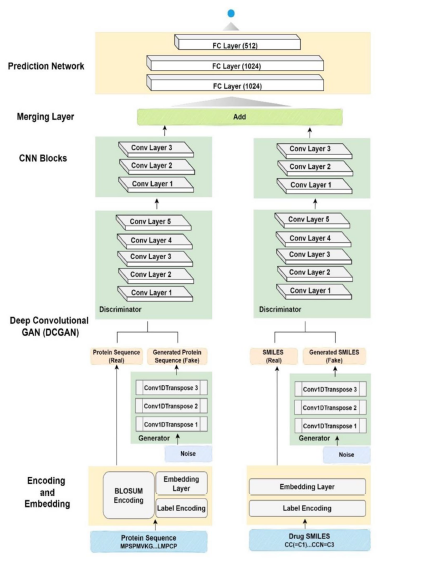
\includegraphics[width=0.96\linewidth]{presentation-figs/DCGAN-block-diagram.png}
    \end{column}

    \begin{column}{0.57\textwidth}
      \begin{block}{پنج مرحله --- شکل از پایین به بالا خوانده می‌شود}
        \footnotesize
        \begin{enumerate}\itemsep0.35ex
          \item کدگذاری و تعبیه --- \e{Label} / \e{BLOSUM} + \e{Embedding}
          \item پیش‌آموزش \e{DCGAN} --- \e{Generator} + \e{Discriminator}
          \item بلوک‌های \e{CNN} --- استخراج ویژگی
          \item لایه‌ی ادغام دو شاخه --- \e{Add}
          \item شبکه‌ی پیش‌بینی --- \e{FC 1024} $\rightarrow$ \e{512}
        \end{enumerate}
      \end{block}

      \vspace{1mm}
      \begin{alertblock}{نکته‌ی کلیدی}
        \footnotesize
        \e{GAN} اینجا \key{برای تولید دارو نیست}؛ \e{Generator} و
        \e{Discriminator} فقط برای \key{پیش‌آموزش نمایش} به کار می‌روند و
        نمایش آموخته‌شده به سر رگرسیون داده می‌شود.
      \end{alertblock}
    \end{column}
  \end{columns}
  \note{شکل را از پایین به بالا توضیح بده --- همان ترتیبی که در ستون کنارش شماره خورده است. دو شاخه‌ی چپ و راست شکل کاملاً متقارن‌اند؛ تنها تفاوت جدی، \e{BLOSUM encoding} در شاخه‌ی پروتئین است که اطلاعات تکاملی (شباهت جانشینی اسیدهای آمینه) را وارد مدل می‌کند. اگر وقت کم بود فقط بگو: کدگذاری، پیش‌آموزش تخاصمی، \e{CNN}، ادغام، رگرسیون.}
\end{frame}

%======================================================================
\section{مقاله‌ی دوم: \e{Co-VAE}}
%======================================================================

%--------------------------------------------------------------- 17 --
\begin{frame}{\e{Co-VAE}}
  \framesubtitle{نماینده‌ی شاخه‌ی \e{VAE} \ --- \ \e{Li, Zhao \& Li}, \e{IEEE TPAMI}, ۲۰۲۲}
  \vspace{3mm}
  \begin{columns}[T]
    \begin{column}{0.50\textwidth}
      \centering
      \begin{tikzpicture}[node distance=5mm,font=\footnotesize]
        \node[drug,minimum width=26mm] (d) {\e{Drug SMILES}};
        \node[model,minimum width=18mm,below=6mm of d] (v1) {\lr{$\text{VAE}_1$}};
        \node[nxn,minimum width=26mm,below=6mm of v1] (dl) {\e{Drug latent}};
        \draw[arr] (d)--(v1); \draw[arr] (v1)--(dl);

        \node[targ,minimum width=26mm,right=10mm of d] (t) {\e{Protein sequence}};
        \node[model,minimum width=18mm,below=6mm of t] (v2) {\lr{$\text{VAE}_2$}};
        \node[nxn,minimum width=26mm,below=6mm of v2] (tl) {\e{Target latent}};
        \draw[arr] (t)--(v2); \draw[arr] (v2)--(tl);

        \node[model,minimum width=34mm,below=8mm of $(dl)!0.5!(tl)$] (co) {\e{Co-regularization}};
        \node[res,minimum width=30mm,below=6mm of co] (af) {\e{Binding affinity}};
        \draw[arr] (dl.south) -- (co.north west);
        \draw[arr] (tl.south) -- (co.north east);
        \draw[arr] (co) -- (af);
      \end{tikzpicture}
    \end{column}

    \begin{column}{0.46\textwidth}
      \small
      \vspace{2mm}
      \begin{block}{ایده‌ی اصلی}
        دو \e{VAE} مجزا برای دارو و هدف، به‌همراه یک بخش
        \key{\e{co-regularization}} که فضاهای نهان را به مقدار
        \e{affinity} گره می‌زند.
      \end{block}

      \vspace{1.5mm}
      \begin{exampleblock}{چرا این مقاله مهم است}
        \footnotesize
        فضای نهان اینجا \key{احتمالاتی} است، نه یک بردار ثابت؛ و مدل فقط برای
        \e{prediction} طراحی نشده --- نویسندگان نشان می‌دهند می‌توان از آن برای
        \key{تولید داروهای جدید با هدف‌های مشابه} نیز استفاده کرد.
      \end{exampleblock}
    \end{column}
  \end{columns}
  \note{تفاوت بنیادی با مقاله‌ی قبل: آنجا نمایش با فرایند تخاصمی و در یک مرحله‌ی پیش‌آموزشِ جدا ساخته می‌شود؛ اینجا فضای نهان احتمالاتی است و بازسازی، هم‌تنظیمی و رگرسیون هم‌زمان آموزش می‌بینند. همین تقابل --- \e{Adversarial} در برابر \e{Variational} --- است که مقایسه‌ی این دو را برای پایان‌نامه ارزشمند می‌کند.}
\end{frame}

%--------------------------------------------------------------- 18 --
\begin{frame}{معماری \e{Co-VAE}}
  \framesubtitle{نمودار بلوکی مقاله --- \e{Li et al.}, \e{IEEE TPAMI}, ۲۰۲۲}
  \vspace{1mm}
  \begin{columns}[c]
    \begin{column}{0.36\textwidth}
      \centering
      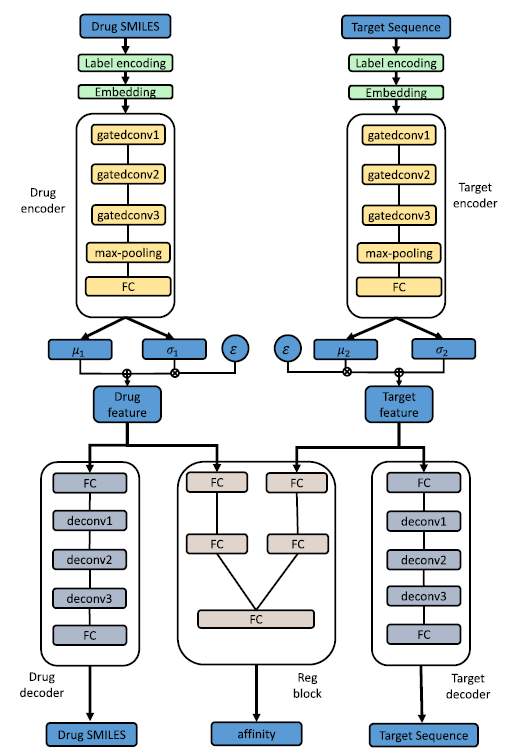
\includegraphics[width=0.94\linewidth]{presentation-figs/coVAE-block-diagram.png}
    \end{column}

    \begin{column}{0.61\textwidth}
      \begin{block}{مسیر بالا به پایین}
        \footnotesize
        \begin{enumerate}\itemsep0.3ex
          \item دو رمزگذار موازی --- \e{gatedconv}$\times$\e{3} + \e{max-pool} + \e{FC}
          \item فضای نهان --- \lr{$\mu$}، \lr{$\sigma$}، \lr{$\varepsilon$} و بازپارامتری‌سازی
        \end{enumerate}
      \end{block}

      \vspace{0.8mm}
      \begin{exampleblock}{سه سر خروجی از \e{drug} / \e{target feature}}
        \footnotesize
        \begin{itemize}\itemsep0.25ex
          \item \e{Drug decoder} --- بازسازی \e{SMILES}
          \item \E{Reg block} --- پیش‌بینی \key{\e{affinity}}
          \item \e{Target decoder} --- بازسازی توالی هدف
        \end{itemize}
      \end{exampleblock}

      \vspace{1.5mm}
      {\footnotesize\color{nxgray}
       همان دو فضای نهان هم‌زمان \key{بازسازی} و \key{رگرسیون} را تغذیه
       می‌کنند؛ همین اشتراک نقش \e{co-regularization} را بازی می‌کند.}
    \end{column}
  \end{columns}
  \note{تفاوت ساختاری مهم با \e{DCGAN-DTA}: آنجا پیش‌آموزش و رگرسیون دو مرحله‌ی جدا بودند، اینجا بازسازی و رگرسیون هم‌زمان و از یک فضای نهان مشترک آموزش می‌بینند. اگر پرسیده شد \e{co-regularization} دقیقاً چیست: یک جمله‌ی اضافه در تابع هزینه، علاوه بر دو جمله‌ی بازسازی و دو جمله‌ی \e{KL}، که فضاهای نهان دارو و هدف را طوری شکل می‌دهد که از رویشان بتوان \e{affinity} را بازیابی کرد.}
\end{frame}

%======================================================================
\section{مقایسه و خلأ پژوهشی}
%======================================================================

%--------------------------------------------------------------- 19 --
\begin{frame}{مقایسه‌ی دو رویکرد}
  \framesubtitle{\e{DCGAN-DTA} در برابر \e{Co-VAE}}
  \vspace{2mm}
  \centering
  {\footnotesize
  \rowcolors{2}{nxlight}{white}
  \begin{tabular}{p{0.22\textwidth} p{0.30\textwidth} p{0.30\textwidth}}
    \rowcolor{nxdark}
    \thd{ویژگی} & \thd{\e{DCGAN-DTA}} & \thd{\e{Co-VAE}} \\
    نوع مدل            & \e{GAN}                          & \e{VAE} \\
    ایده‌ی اصلی        & \e{Adversarial learning}         & \e{Variational learning} \\
    اجزا               & \e{Generator} + \e{Discriminator}& \e{Encoder} + \e{Decoder} \\
    فضای نهان          & تخاصمی / مولد                    & احتمالاتی \\
    نمایش دارو         & \e{SMILES}                       & \e{SMILES} \\
    نمایش هدف          & \e{Protein sequence}             & \e{Protein sequence} \\
    خروجی              & \e{Prediction}                   & \e{Prediction} + \e{co-regularization} \\
    هدف جانبی          & یادگیری نمایش                    & تولید + یادگیری نمایش \\
  \end{tabular}}

  \vspace{4mm}
  \begin{alertblock}{جمله‌ی کلیدی}
    \centering
    تفاوت اصلی این دو مقاله فقط در \e{architecture} نیست؛ آن‌ها
    \key{دو دیدگاه متفاوت} نسبت به یادگیری نمایش دارند.
  \end{alertblock}
  \note{این جدول را سطر به سطر نخوان. فقط سه سطر اول را بگو و مستقیم برو سراغ جمله‌ی پایین اسلاید، چون همان جمله ورودی بخش نوآوری است.}
\end{frame}

%--------------------------------------------------------------- 20 --
\begin{frame}{خلأ پژوهشی}
  \framesubtitle{\e{Research Gap}}
  \vspace{3mm}
  \begin{columns}[T]
    \begin{column}{0.47\textwidth}
      \begin{block}{\e{DCGAN-DTA}}
        \small تمرکز بر یادگیری نمایش مبتنی بر \e{GAN} برای \e{DTA}.
      \end{block}
      \vspace{2mm}
      \begin{exampleblock}{\e{Co-VAE}}
        \small تمرکز بر نمایش وردشی به‌همراه \e{co-regularization} برای \e{DTA}.
      \end{exampleblock}
    \end{column}

    \begin{column}{0.49\textwidth}
      \centering
      \vspace{1mm}
      \begin{tikzpicture}[font=\footnotesize,node distance=5mm]
        \node[nxn,minimum width=24mm,fill=nxblue!18,draw=nxblue!80] (a) {\e{DCGAN-DTA}};
        \node[nxn,minimum width=24mm,right=10mm of a,fill=nxteal!18,draw=nxteal!80] (b) {\e{Co-VAE}};
        \node[ghost,minimum width=40mm,below=10mm of $(a)!0.5!(b)$,draw=nxred!70,dashed,text=nxred]
          (g) {\fa{پروتکل آزمایشی مشترک؟}};
        \draw[arrd,draw=nxred!70] (a) -- (g);
        \draw[arrd,draw=nxred!70] (b) -- (g);
      \end{tikzpicture}
    \end{column}
  \end{columns}

  \vspace{4mm}
  \begin{alertblock}{خلأ}
    \centering
    مقایسه‌ی \key{مستقیم و کنترل‌شده}ی این دو پارادایم تحت یک
    \e{experimental protocol} مشترک، مسئله‌ای است که در این پایان‌نامه بررسی می‌شود.
  \end{alertblock}
  \note{اینجا محتاط باش و ادعای بزرگ نکن. نگو «هیچ‌کس این کار را نکرده»؛ بگو «تا جایی که بررسی کرده‌ام، مقایسه‌ی کنترل‌شده‌ی این دو خانواده تحت یک پروتکل یکسان کمتر انجام شده است». این جمله قابل دفاع‌تر است.}
\end{frame}

%======================================================================
\section{نوآوری پیشنهادی}
%======================================================================

%--------------------------------------------------------------- 21 --
\begin{frame}{نوآوری‌های پیشنهادی}
  \framesubtitle{چهار محور اصلی پایان‌نامه}
  \vspace{3mm}
  \begin{columns}[T]
    \begin{column}{0.48\textwidth}
      \small
      \begin{block}{۱. مقایسه‌ی دو پارادایم مولد}
        \e{Adversarial learning} در برابر \e{Variational learning}
        برای مسئله‌ی \e{DTA}.
      \end{block}

      \vspace{1mm}
      \begin{block}{۲. پروتکل آزمایشی یکسان}
        مجموعه‌داده، \e{preprocessing}، نمایش‌ها، \e{split}، معیارها و
        \e{seed}های کنترل‌شده --- تا تفاوت عملکرد واقعاً به
        \e{architecture} نسبت داده شود.
      \end{block}
    \end{column}

    \begin{column}{0.48\textwidth}
      \small
      \begin{block}{۳. بررسی \e{generalization}}
        مقایسه در دو شرایط \e{warm-start} و \e{cold-start}؛ عملکرد روی
        \e{random split} لزوماً توان پیش‌بینی برای داروها و هدف‌های
        واقعاً جدید را نشان نمی‌دهد.
      \end{block}

      \vspace{1mm}
      \begin{block}{۴. تحلیل فراتر از دقت}
        علاوه بر \e{performance}: \e{generalization}،
        \e{training stability}، \e{computational cost} و
        \e{data efficiency}.
      \end{block}
    \end{column}
  \end{columns}

  \vspace{3mm}
  \centering
  {\footnotesize\color{nxgray}
   \e{DCGAN-DTA} نیز همین مسئله را با \e{warm-start} و \e{cold-start} فیزیکوشیمیایی مورد توجه قرار داده است.}
  \note{مهم‌ترین اسلاید دفاع از نوآوری. اگر استاد گفت «این فقط مقایسه است، نوآوری نیست»، پاسخ آماده داشته باش: نوآوری در طراحی پروتکل کنترل‌شده و در تحلیل چندبعدی (نه صرفاً عدد دقت) است، و خروجی آن یک راهنمای انتخاب مدل برای این حوزه است.}
\end{frame}

%--------------------------------------------------------------- 22 --
\begin{frame}{سؤال اصلی پژوهش}
  \framesubtitle{پرسش اصلی و پرسش‌های فرعی}
  \vspace{2mm}
  \begin{alertblock}{پرسش اصلی}
    \centering
    آیا نوع روش یادگیری مولد --- \key{تخاصمی} یا \key{وردشی} --- می‌تواند بر
    کیفیت یادگیری نمایش و عملکرد پیش‌بینی قدرت اتصال در مسئله‌ی \e{DTA}
    تأثیر معناداری داشته باشد؟
  \end{alertblock}

  \vspace{1.5mm}
  \begin{block}{پرسش‌های فرعی}
    \footnotesize
    \begin{enumerate}\itemsep0.35ex
      \item کدام روش در \e{warm-start} عملکرد بهتری دارد؟
      \item کدام روش در \e{cold-start} بهتر \e{generalize} می‌کند؟
      \item حساسیت هر مدل نسبت به حجم داده چقدر است؟
      \item کدام مدل از نظر \e{computational cost} مناسب‌تر است؟
      \item آیا برتری مشاهده‌شده ناشی از \e{architecture} است یا از
            \e{dataset} / \e{split} / \e{preprocessing}؟
    \end{enumerate}
  \end{block}
  \note{ارائه باید با همین اسلاید به اوج برسد. پرسش پنجم مهم‌ترین است و نشان می‌دهد به اعتبار درونی آزمایش فکر کرده‌ای؛ روی همان یک مکث کوتاه کن.}
\end{frame}

%--------------------------------------------------------------- 23 --
\begin{frame}{روایت کلی ارائه}
  \framesubtitle{جمع‌بندی بصری مسیر ارائه}
  \vspace{3mm}
  \centering
  % سه سطر: صورت‌مسئله، مسیر روش‌ها، و جمع‌بندی به نوآوری
  \begin{tikzpicture}[x=1mm,y=1mm,font=\scriptsize]
    % --- row 1: the problem ---
    \node[ghost,minimum width=20mm] (dti) at (14,24) {\e{DTI}};
    \node[ghost,minimum width=20mm] (dta) at (44,24) {\e{DTA}};
    \node[nxn,minimum width=30mm]   (aff) at (84,24) {\e{Binding affinity}};
    \draw[arr] (dti)--(dta); \draw[arr] (dta)--(aff);
    % برچسب‌ها بالای سطر اول تا مسیر اتصال به سطر دوم آزاد بماند
    \node[lbl,text width=22mm,align=center] at (14,32) {\fa{هست یا نیست؟}};
    \node[lbl,text width=22mm,align=center] at (44,32) {\fa{چقدر قوی؟}};
    \node[lbl,text width=30mm,align=center] at (84,32) {\e{Kd} / \e{Ki} / \e{IC50}};

    % --- row 2: how the field got here ---
    \node[ghost,minimum width=18mm] (cls) at (11,4)  {\fa{کلاسیک}};
    \node[ghost,minimum width=13mm] (mlx) at (33,4)  {\e{ML}};
    \node[model,minimum width=13mm] (dlx) at (53,4)  {\e{DL}};
    \node[model,minimum width=32mm] (rep) at (87,4)  {\e{Representation learning}};
    \node[res,minimum width=18mm]   (gen) at (117,4) {\fa{مدل‌های مولد}};
    \draw[arr] (cls)--(mlx); \draw[arr] (mlx)--(dlx);
    \draw[arr] (dlx)--(rep); \draw[arr] (rep)--(gen);
    \draw[arr] (aff.south) -- ++(0,-6) -| (cls.north);

    % --- row 3: the two papers, the comparison, the contribution ---
    \node[nxn,minimum width=24mm,fill=nxblue!18,draw=nxblue!80] (g1) at (14,-16) {\e{DCGAN-DTA}};
    \node[nxn,minimum width=18mm,fill=nxteal!18,draw=nxteal!80] (g2) at (42,-16) {\e{Co-VAE}};
    \node[nxn,minimum width=30mm,draw=nxred!70,fill=nxred!8]    (cmp) at (80,-16) {\fa{مقایسه‌ی کنترل‌شده}};
    \node[res,minimum width=26mm,fill=nxaccent!30,draw=nxaccent] (nov) at (115,-16) {\fa{نوآوری پایان‌نامه}};
    \draw[arr] (g1)--(g2);
    \draw[arr] (g2)--(cmp);
    \draw[arr] (cmp)--(nov);
    \draw[arr] (gen.south) -- ++(0,-5) -| (g1.north);
  \end{tikzpicture}
  \note{این اسلاید جمع‌بندی بصری است. می‌توانی آن را ۱۵ ثانیه‌ای رد کنی یا اگر جلسه طولانی شد مستقیم از اسلاید ۲۲ به اسلاید پرسش‌ها بروی.}
\end{frame}

%--------------------------------------------------------------- 24 --
\begin{frame}{مراجع اصلی}
  \framesubtitle{منابع کلیدی این ارائه}
  \vspace{4mm}
  \small
  % هر مرجع یک بازه‌ی کامل چپ‌به‌راست است تا ترتیب اجزای استناد به‌هم نریزد
  \vspace{-2mm}
  \begin{enumerate}\footnotesize\itemsep0.35ex
    \item \lr{Wang et al., \textit{A unified survey on drug--target interaction
          and binding affinity prediction}, Biotechnology Advances, 2026.}
    \item \lr{Pahikkala et al., \textit{Toward more realistic drug--target
          interaction predictions} (KronRLS), Brief.\ Bioinform., 2015.}
    \item \lr{He et al., \textit{SimBoost: a read-across approach using gradient
          boosting machines}, J.\ Cheminformatics, 2017.}
    \item \lr{Öztürk et al., \textit{DeepDTA: deep drug--target binding affinity
          prediction}, Bioinformatics, 2018.}
    \item \lr{Öztürk et al., \textit{WideDTA: prediction of drug--target binding
          affinity}, arXiv, 2019.}
    \item \lr{Nguyen et al., \textit{GraphDTA: predicting drug--target binding
          affinity with graph neural networks}, Bioinformatics, 2021.}
    \item \lr{Li et al., \textit{Co-VAE: Drug--Target Binding Affinity Prediction
          by Co-Regularized Variational Autoencoders}, IEEE TPAMI, 2022.}
    \item \lr{Kalemati et al., \textit{DCGAN-DTA: Predicting drug--target binding
          affinity with deep convolutional GANs}, BMC Genomics, 2024.}
  \end{enumerate}

  \vspace{4mm}
  {\footnotesize\color{nxgray}
   فهرست کامل مراجع در متن پایان‌نامه ارائه شده است.}
  \note{این اسلاید فقط برای مستند بودن است؛ روی آن توقف نکن مگر استاد سؤال کند.}
\end{frame}

%--------------------------------------------------------------- 25 --
\begin{frame}[plain,noframenumbering]
  \vfill
  \begin{center}
    {\lr{\textcolor{nxaccent}{\rule{28mm}{1.6pt}}}}\\[6mm]
    {\Large\bfseries\color{nxdark} با تشکر از توجه شما}\\[5mm]
    {\large\color{nxgray} پرسش‌ها و پیشنهادها}\\[8mm]
    {\small محسن کاشفی کیا \quad$\cdot$\quad استاد راهنما: دکتر سایه میرزایی}
  \end{center}
  \vfill
  \note{آماده باش برای این سه سؤال: (۱) چرا همین دو مقاله را انتخاب کردی؟ (۲) داده و منابع محاسباتی را چطور تأمین می‌کنی؟ (۳) اگر نتیجه این شد که تفاوت معنادار نیست، دستاورد پایان‌نامه چیست؟ برای سؤال سوم پاسخ بده: نتیجه‌ی منفی هم یافته است، چون نشان می‌دهد تفاوت گزارش‌شده در مقالات ناشی از پروتکل بوده نه معماری.}
\end{frame}

\end{document}
